\chapter{Ergebnisse}
\label{chapter:ergebnisse}

In diesem Kapitel werden die vier Browser Mozilla Firefox, Tor-Browser, Google Chrome sowie Brave gemäß definierter Methodik in Kapitel \ref{chapter:methodik} analysiert. Dabei wird für jeden Browser untersucht, ob Private-Browsing-Artefakte in den Common Locations, Uncommon Locations und der Registry hinterlassen wurden. 

% Hier evtl. noch schreiben, dass Ausführliche Analyse im Anhang zu finden ist

\section{Firefox}
\label{section:ergebnisse-firefox}
Im nachfolgenden Abschnitt werden die Ergebnisse der Datenanalyse für den Webbrowser Firefox beschrieben. Die Analyse ist in drei Hauptkategorien unterteilt: Common Locations, Uncommon Locations und Registry.

\subsection*{Common Locations}
\label{subsection:ergebnisse-firefox-commonlocations}
Zunächst werden die Common Locations nach potenziellen privaten Browsing-Artefakten untersucht. In diesem Versuch wurde gemäß Methodik in Abschnitt \ref{subsection:methodik-datenanalyse-commonlocations} zwischen Datei-Schreiboperationen aus den Process Monitor Logfiles und SQLite-Datenbanken zur Verwaltung von Nutzerdaten unterschieden. Weder in den Schreiboperationen der Process Monitor Logfiles noch in den SQLite-Datenbanken konnten PB-Artefakte gefunden werden. 

Eine detaillierte Analyse der untersuchten Dateien ist im Anhang \ref{subsection:appendix-firefox-common-locations} beschrieben.

\subsection*{Uncommon Locations}
\label{subsection:ergebnisse-firefox-uncommonlocations}
Nachfolgend werden die Analyseergebnisse der Firefox Uncommon Locations beschrieben.
Im Gegensatz zu den Common Locations benötigt ein Forensiker dabei kein Wissen über das Browserverhalten. Stattdessen wird sich auf die Vollständigkeit der Funktionen von Forensik-Tools verlassen. Im Rahmen dieses Versuchs werden die Tools Autopsy und Volatility verwendet.

\subsubsection*{Analyse mit Autopsy}
\label{subsubsection:ergebnisse-firefox-uncommonlocations-analysemitautopsy}
Zur Analyse der Common Locations in Abschnitt \ref{subsection:ergebnisse-firefox-commonlocations} wird Autopsy zur Dateiextraktion genutzt. Im Falle der Uncommon Locations dient Autopsy zusätzlich als forensisches Werkzeug zur Datenanalyse.

Eine Autopsy Stichwortsuche gemäß Methodik in Abschnitt \ref{subsubsection:methodik-datenanalyse-uncommonlocations-analysemitautopsy} lieferte in allen Snapshots keine Treffer. Dabei wurde zusätzlich das \texttt{\$Carved} Verzeichnis durchsucht, in dem Autopsy alle wiederhergestellten Dateien speichert.

Ebenso wurden in den von Autopsy automatisch kategorisierten Dateien keine PB-Artefakte gefunden. Eine detaillierte Analyse der Kategorien \glqq{}Web Bookmarks\grqq{}, \glqq{}Web Cookies\grqq{}, \glqq{}Web History\grqq{} sowie \glqq{}Web Categories\grqq{} ist im Anhang \ref{subsubsection:appendix-firefox-uncommon-locations-autopsy} beschrieben.

\subsubsection*{Analyse mit Volatility}
\label{subsubsection:ergebnisse-firefox-uncommonlocations-analysemitvolatility}
Zur Untersuchung des RAM als Uncommon Location wurde eine Stringsuche in den gesamten Arbeitsspeicherabbildern nach PB-Artefakten durchgeführt.
Wie in Abschnitt \ref{subsubsection:methodik-datenanalyse-uncommonlocations-analysemitvolatility} ausführlich beschrieben, muss ein gefundener String eindeutig einem Browser zugeordnet werden können. 
Dazu wird mit dem Volatility PlugIn \textit{Yarascan} nach den in Anhang \ref{appendix:yara-regeln} aufgeführten Yara-Regeln im RAM gesucht. Davon ausgehend wird das Plug-In \textit{pslist} verwendet, um den Prozessnamen anhand PID zu identifizieren.
Die Ergebnisse dieser Stringsuche sind nachfolgend nach den Yara-Regeln geordnet.

\paragraph*{Yara-Regel \glqq{}HTML\grqq{}}
In keinem der Firefox RAM-Dumps wurden HTML-Fragemente der besuchten Seiten gefunden. Somit wird diese Yara-Regel nicht weiter betrachtet.

\paragraph*{Yara-Regel \glqq{}Suchbegriffe\grqq{}}
Wie in Tabelle \ref{chart:firefox-volatility-keywords} gezeigt, wurden die Suchbegriffe \glqq{}pfaffenhofen\grqq{}, \glqq{}nanoradar\grqq{}, \glqq{}mooserliesl\grqq{} sowie \glqq{}mallofamerica\grqq{} ausschließlich nach dem Browsing-Szenario mit geöffnetem Browser (RAM-Dump 2) identifiziert. Die Suchbegriffe wurden größtenteils in den Speicherbereichen von Firefox-Prozessen gefunden. Nur in elf Fällen wurden Suchbegriffe in diversen anderen Prozessen des Betriebssystems identifiziert. Am häufigsten wurde der Suchbegriff \glqq{}pfaffenhofen\grqq{} mit 1301 Artefakten gefunden. Dies ist vermutlich auf den  visuellen Google Maps Kartenausschnitt zurückzuführen, welcher bei der Google-Suche relevante Informationen über die gesuchte Stadt zeigt. 

\begin{table}[h!]
	\resizebox{\linewidth}{!}{
	\begin{tabular}{l}	
		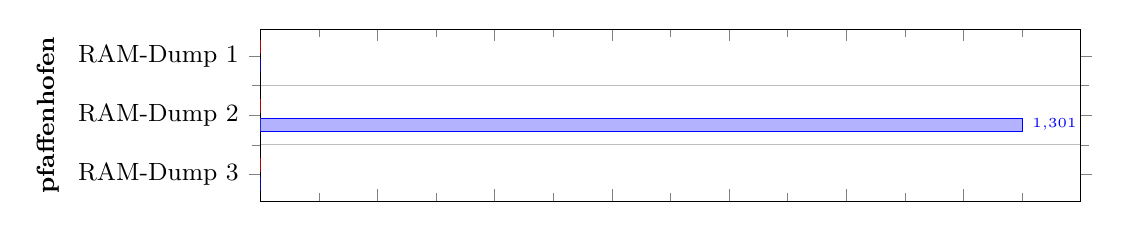
\begin{tikzpicture}
			\begin{axis}[
			xbar,
			width=12cm, 
			height=3cm, 
			ylabel style={align=center}, ylabel=\textbf{pfaffenhofen},
			y=0.75cm,
			symbolic y coords={RAM-Dump 3, RAM-Dump 2, RAM-Dump 1},
			label style={font=\small},
			tick label style={font=\small},
			ytick=data,
			xticklabels={,,},
            xmin = 0,
            xmax = 1400,
			nodes near coords, 
			nodes near coords align={horizontal},
			nodes near coords style={font=\tiny},
   			nodes near coords={\pgfmathfloatifflags{\pgfplotspointmeta}{0}{}{\pgfmathprintnumber{\pgfplotspointmeta}}},
			bar width=.17cm,
			enlarge y limits={abs=2*\pgfplotbarwidth},
			scaled x ticks=false,
			legend style={
				at={(0.5,-0.1)},
				anchor=north
			},
			legend columns=3,
    		yminorgrids = true,minor tick num=1
			]
				\addplot coordinates {
				(0,RAM-Dump 3) (1301,RAM-Dump 2) (0,RAM-Dump 1)
				};
				\addplot coordinates {
				(0,RAM-Dump 3) (0,RAM-Dump 2) (0,RAM-Dump 1)
				};
			\end{axis}
		\end{tikzpicture}
		\\[-7pt]
		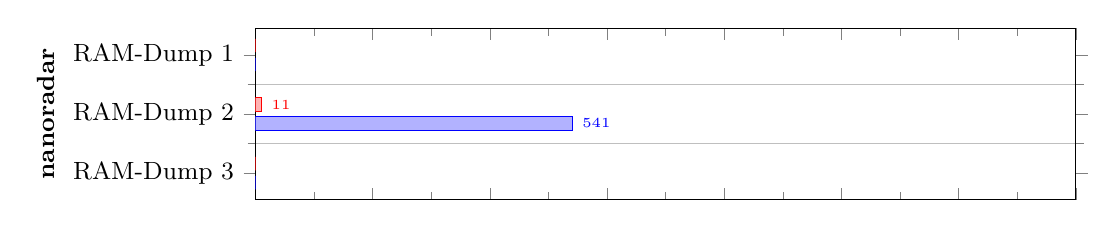
\begin{tikzpicture}
			\begin{axis}[
			xbar,
			width=12cm, 
			height=3cm, 
			ylabel style={align=center}, ylabel=\textbf{nanoradar},
			y=0.75cm,
			symbolic y coords={RAM-Dump 3, RAM-Dump 2, RAM-Dump 1},
			label style={font=\small},
			tick label style={font=\small},
			ytick=data,
			xticklabels={,,},
            xmin = 0,
            xmax = 1400,
			nodes near coords, 
			nodes near coords align={horizontal},
			nodes near coords style={font=\tiny},
   			nodes near coords={\pgfmathfloatifflags{\pgfplotspointmeta}{0}{}{\pgfmathprintnumber{\pgfplotspointmeta}}},
			bar width=.17cm,
			enlarge y limits={abs=2*\pgfplotbarwidth},
			scaled x ticks=false,
			legend style={
				at={(0.5,-0.1)},
				anchor=north
			},
			legend columns=3,
    		yminorgrids = true,minor tick num=1
			]
				\addplot coordinates {
				(0,RAM-Dump 3)  (541,RAM-Dump 2) (0,RAM-Dump 1)
				};
				\addplot coordinates {
				(0,RAM-Dump 3)  (11,RAM-Dump 2) (0,RAM-Dump 1)
				};
			\end{axis}
		\end{tikzpicture}
		\\[-7pt]
		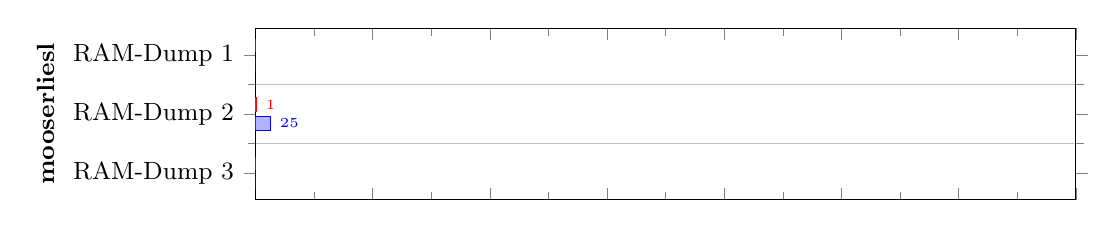
\begin{tikzpicture}
			\begin{axis}[
			xbar,
			width=12cm, 
			height=3cm, 
			ylabel style={align=center}, ylabel=\textbf{mooserliesl},
			y=0.75cm,
			symbolic y coords={RAM-Dump 3, RAM-Dump 2, RAM-Dump 1},
			label style={font=\small},
			tick label style={font=\small},
			ytick=data,
			xticklabels={,,},
            xmin = 0,
            xmax = 1400,
			nodes near coords, 
			nodes near coords align={horizontal},
			nodes near coords style={font=\tiny},
   			nodes near coords={\pgfmathfloatifflags{\pgfplotspointmeta}{0}{}{\pgfmathprintnumber{\pgfplotspointmeta}}},
			bar width=.17cm,
			enlarge y limits={abs=2*\pgfplotbarwidth},
			scaled x ticks=false,
			legend style={
				at={(0.5,-0.1)},
				anchor=north
			},
			legend columns=3,
    		yminorgrids = true,minor tick num=1
			]
				\addplot coordinates {
				(0,RAM-Dump 3)  (25,RAM-Dump 2) (0,RAM-Dump 1)
				};
				\addplot coordinates {
				(0,RAM-Dump 3)  (1,RAM-Dump 2) (0,RAM-Dump 1)
				};
			\end{axis}
		\end{tikzpicture}
		\\[-7pt]
		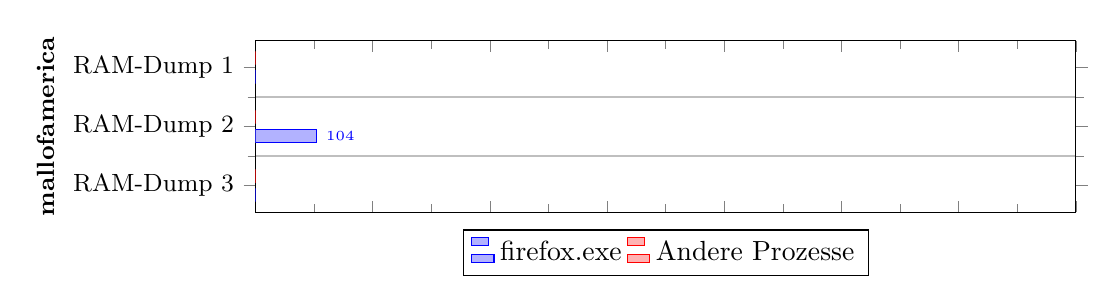
\begin{tikzpicture}
			\begin{axis}[
			xbar,
			width=12cm, 
			height=3cm, 
			ylabel style={align=center}, ylabel=\textbf{mallofamerica},
			y=0.75cm,
			symbolic y coords={RAM-Dump 3, RAM-Dump 2, RAM-Dump 1},
			label style={font=\small},
			tick label style={font=\small},
			ytick=data,
			xticklabels={,,},
            xmin = 0,
            xmax = 1400,
			nodes near coords, 
			nodes near coords align={horizontal},
			nodes near coords style={font=\tiny},
   			nodes near coords={\pgfmathfloatifflags{\pgfplotspointmeta}{0}{}{\pgfmathprintnumber{\pgfplotspointmeta}}},
			bar width=.17cm,
			enlarge y limits={abs=2*\pgfplotbarwidth},
			scaled x ticks=false,
			legend style={
				at={(0.5,-0.1)},
				anchor=north
			},
			legend columns=3,
    		yminorgrids = true,minor tick num=1
			]
				\addplot coordinates {
				(0,RAM-Dump 3)  (104,RAM-Dump 2) (0,RAM-Dump 1)
				};
				\addplot coordinates {
				(0,RAM-Dump 3)  (0,RAM-Dump 2) (0,RAM-Dump 1)
				};
				\legend{firefox.exe, Andere Prozesse}
			\end{axis}
		\end{tikzpicture}
	\end{tabular}
	}
	\captionof{figure}{Firefox: Anzahl gefundener Suchbegriffe im RAM}
	\label{chart:firefox-volatility-keywords}
\end{table}
				

%\begin{figure}[h!]
%	\centerline{\resizebox{\linewidth}{!}{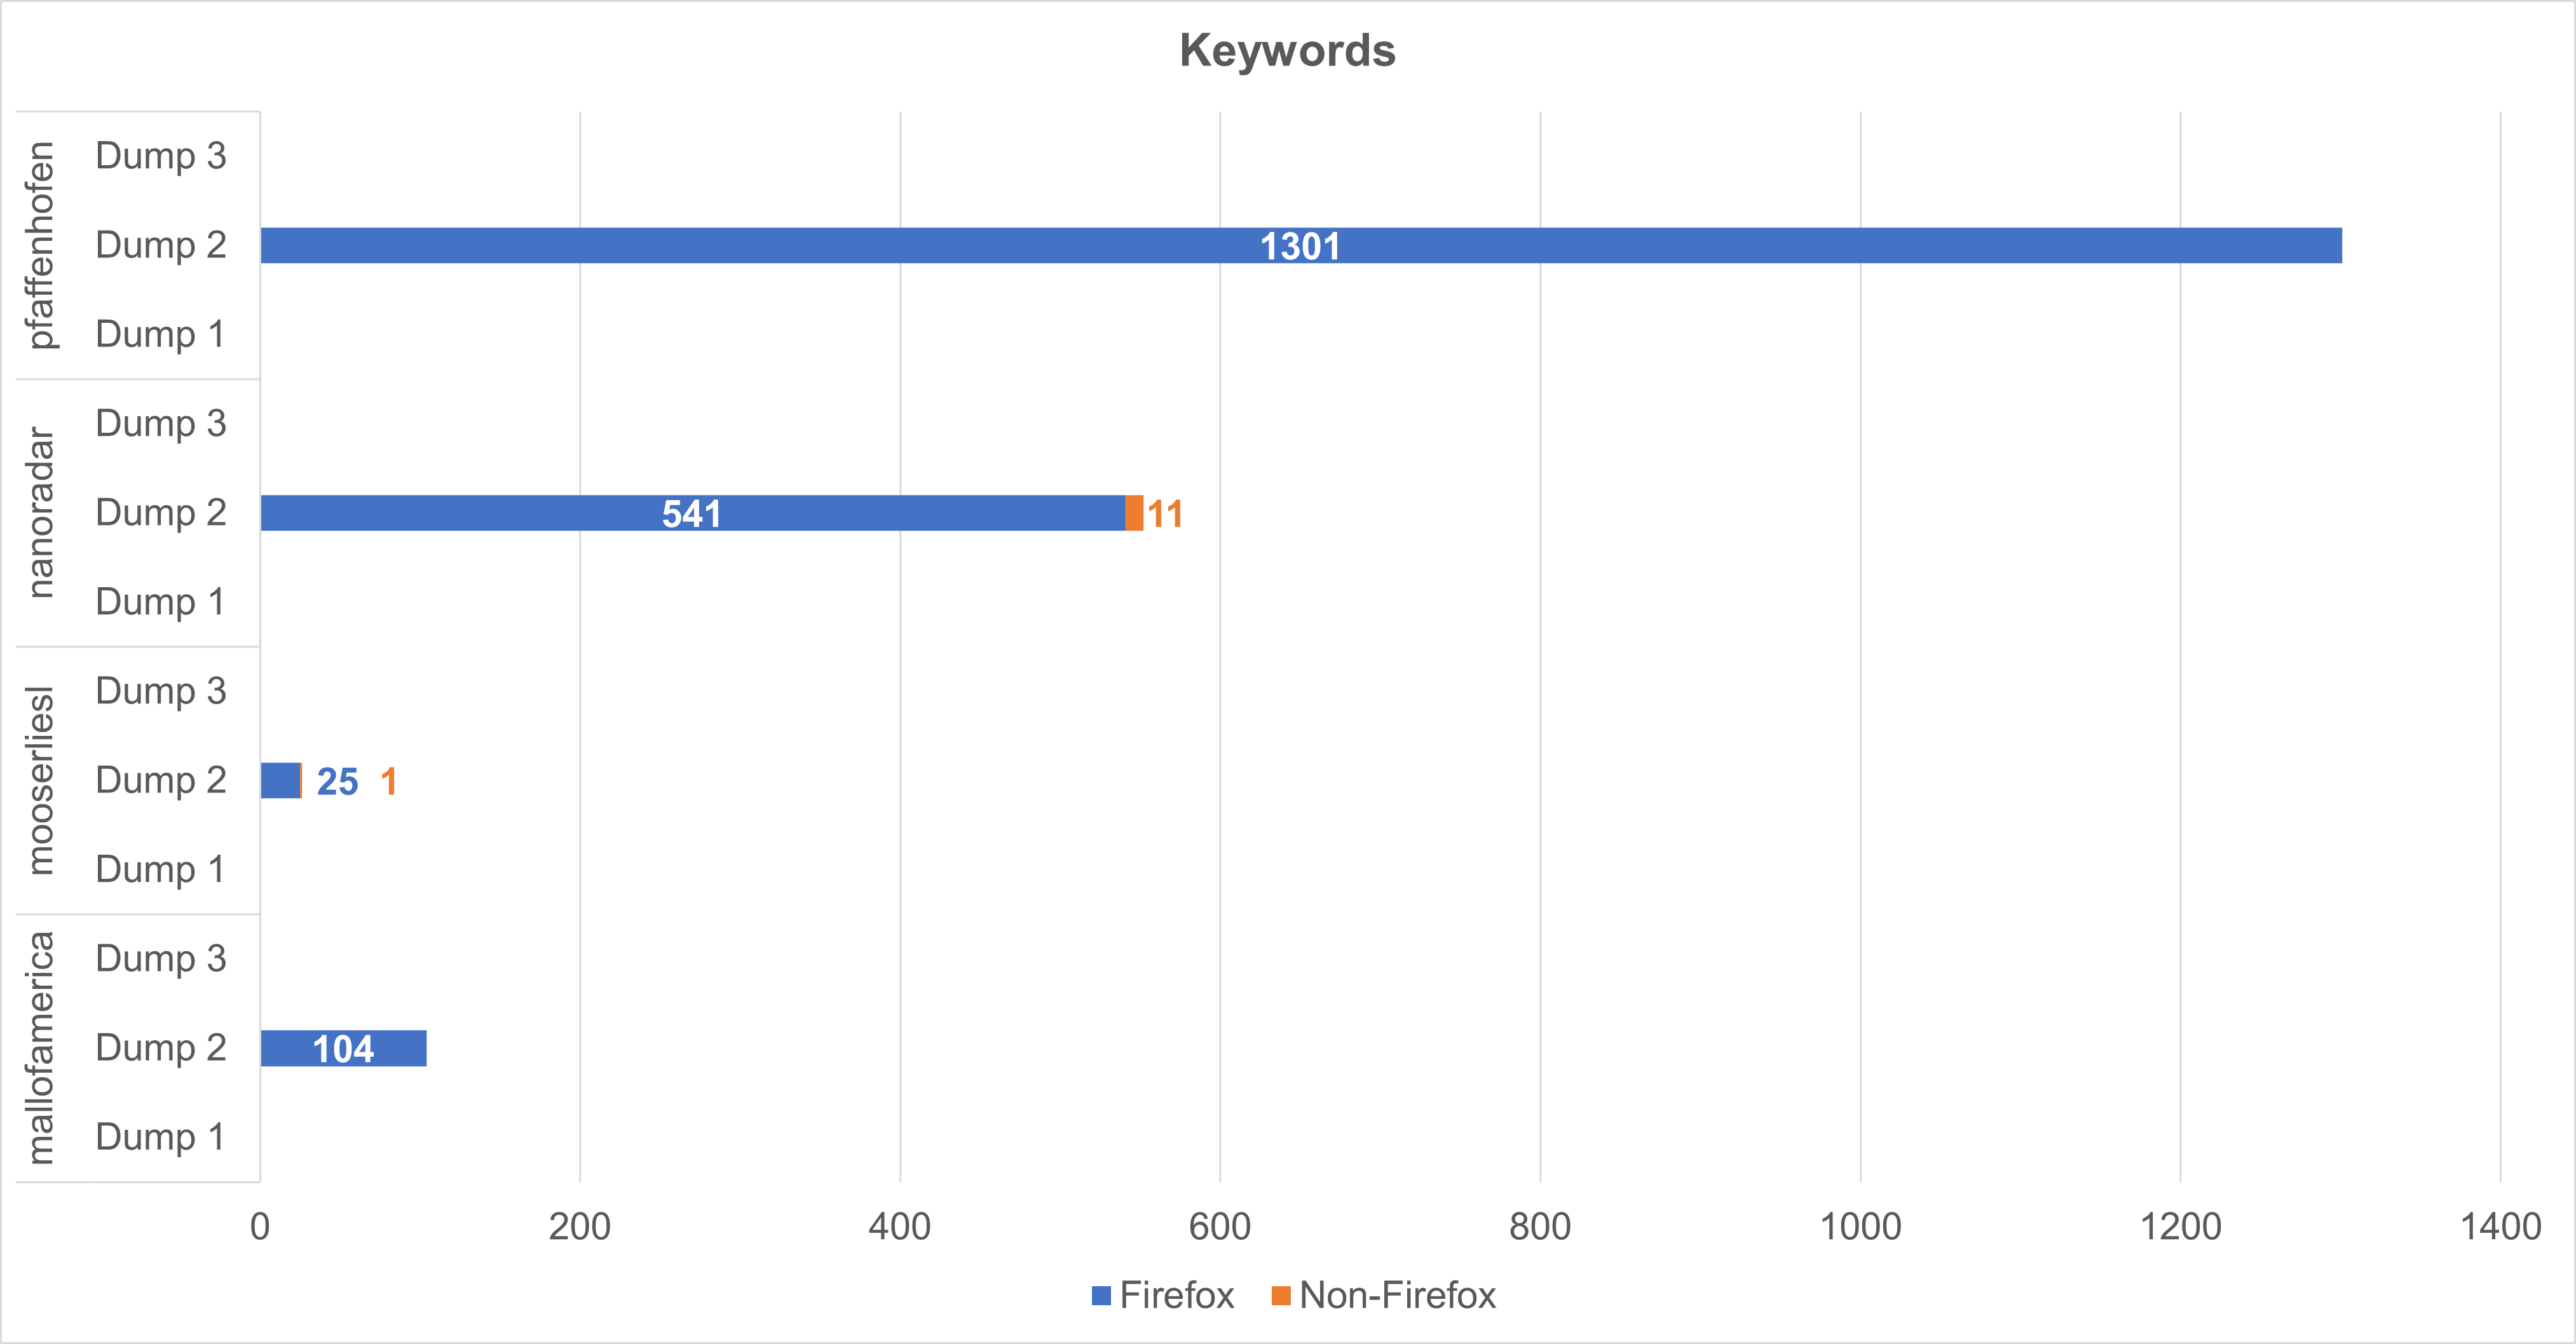
\includegraphics{bilder/volatility/firefox/keywords.png}}}
%	\label{chart:final-criteria}  
%	\caption{Keywords}
%\end{figure}

\paragraph*{Yara-Regel \glqq{}URLs\grqq{}}

\begin{table}[h!]
	\resizebox{\linewidth}{!}{
	\begin{tabular}{r}	
		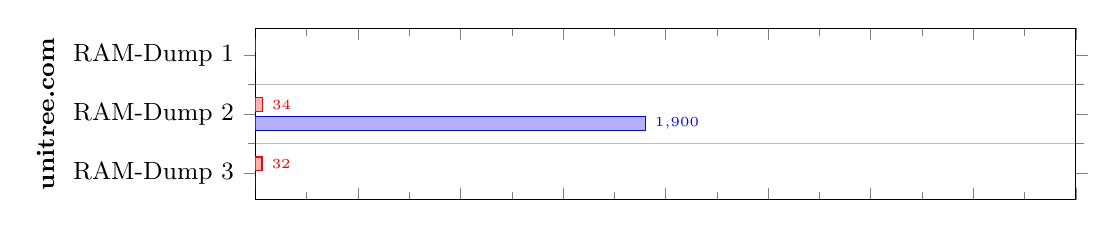
\begin{tikzpicture}
			\begin{axis}[
			xbar,
			width=12cm, 
			height=3cm, 
			ylabel style={align=center}, ylabel=\textbf{unitree.com},
			y=0.75cm,
			symbolic y coords={RAM-Dump 3, RAM-Dump 2, RAM-Dump 1},
			label style={font=\small},
			tick label style={font=\small},
			ytick=data,
			xticklabels={,,},
            xmin = 0,
            xmax = 4000,
			nodes near coords, 
			nodes near coords align={horizontal},
			nodes near coords style={font=\tiny},
   			nodes near coords={\pgfmathfloatifflags{\pgfplotspointmeta}{0}{}{\pgfmathprintnumber{\pgfplotspointmeta}}},
			bar width=.17cm,
			enlarge y limits={abs=2*\pgfplotbarwidth},
			scaled x ticks=false,
			legend style={
				at={(0.5,-0.1)},
				anchor=north
			},
			legend columns=3,
    		yminorgrids = true,minor tick num=1
			]
				\addplot coordinates {
				(0,RAM-Dump 3) (1900,RAM-Dump 2) (0,RAM-Dump 1)
				};
				\addplot coordinates {
				(32,RAM-Dump 3) (34,RAM-Dump 2) (0,RAM-Dump 1)
				};
			\end{axis}
		\end{tikzpicture}
		\\[-7pt]
		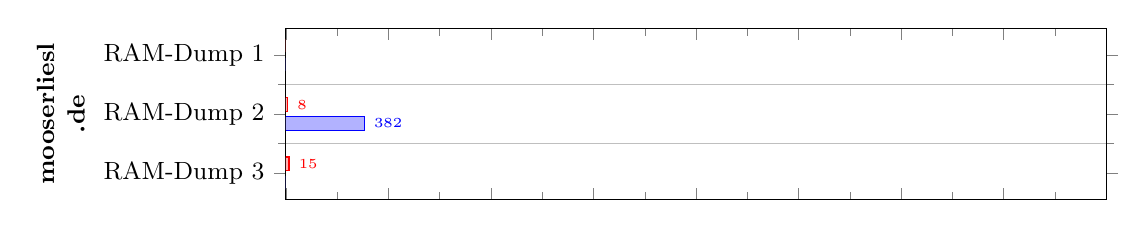
\begin{tikzpicture}
			\begin{axis}[
			xbar,
			width=12cm, 
			height=3cm, 
			ylabel style={align=center}, ylabel=\textbf{mooserliesl}\\\textbf{.de},
			y=0.75cm,
			symbolic y coords={RAM-Dump 3, RAM-Dump 2, RAM-Dump 1},
			label style={font=\small},
			tick label style={font=\small},
			ytick=data,
			xticklabels={,,},
            xmin = 0,
            xmax = 4000,
			nodes near coords, 
			nodes near coords align={horizontal},
			nodes near coords style={font=\tiny},
   			nodes near coords={\pgfmathfloatifflags{\pgfplotspointmeta}{0}{}{\pgfmathprintnumber{\pgfplotspointmeta}}},
			bar width=.17cm,
			enlarge y limits={abs=2*\pgfplotbarwidth},
			scaled x ticks=false,
			legend style={
				at={(0.5,-0.1)},
				anchor=north
			},
			legend columns=3,
    		yminorgrids = true,minor tick num=1
			]
				\addplot coordinates {
				(0,RAM-Dump 3) (382,RAM-Dump 2) (0,RAM-Dump 1)
				};
				\addplot coordinates {
				(15,RAM-Dump 3) (8,RAM-Dump 2) (0,RAM-Dump 1)
				};
			\end{axis}
		\end{tikzpicture}	
		\\[-7pt]
		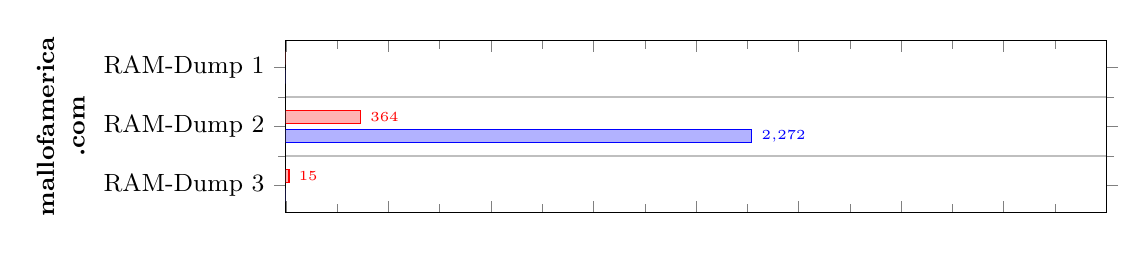
\begin{tikzpicture}
			\begin{axis}[
			xbar,
			width=12cm, 
			height=3cm, 
			ylabel style={align=center}, ylabel=\textbf{mallofamerica}\\\textbf{.com},
			y=0.75cm,
			symbolic y coords={RAM-Dump 3, RAM-Dump 2, RAM-Dump 1},
			label style={font=\small},
			tick label style={font=\small},
			ytick=data,
			xticklabels={,,},
            xmin = 0,
            xmax = 4000,
			nodes near coords, 
			nodes near coords align={horizontal},
			nodes near coords style={font=\tiny},
   			nodes near coords={\pgfmathfloatifflags{\pgfplotspointmeta}{0}{}{\pgfmathprintnumber{\pgfplotspointmeta}}},
			bar width=.17cm,
			enlarge y limits={abs=2*\pgfplotbarwidth},
			scaled x ticks=false,
			legend style={
				at={(0.5,-0.1)},
				anchor=north
			},
			legend columns=3,
    		yminorgrids = true,minor tick num=1
			]
				\addplot coordinates {
				(0,RAM-Dump 3) (2272,RAM-Dump 2) (0,RAM-Dump 1)
				};
				\addplot coordinates {
				(15,RAM-Dump 3) (364,RAM-Dump 2) (0,RAM-Dump 1)
				};
			\end{axis}
		\end{tikzpicture}
		\\[-7pt]
		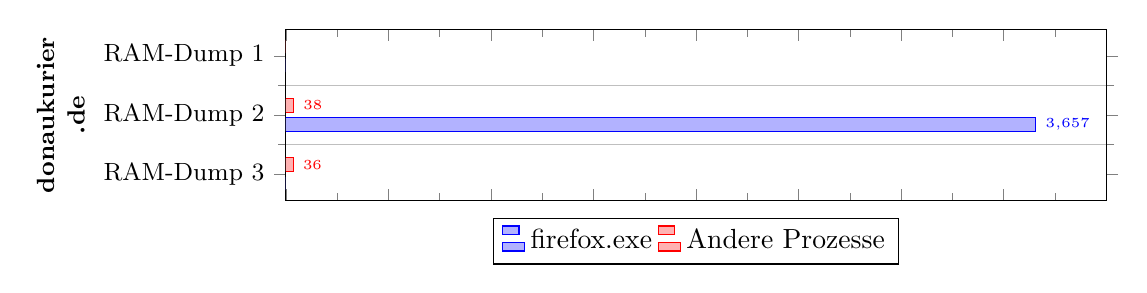
\begin{tikzpicture}
			\begin{axis}[
			xbar,
			width=12cm, 
			height=3cm, 
			ylabel style={align=center}, ylabel=\textbf{donaukurier}\\\textbf{.de},
			y=0.75cm,
			symbolic y coords={RAM-Dump 3, RAM-Dump 2, RAM-Dump 1},
			label style={font=\small},
			tick label style={font=\small},
			ytick=data,
			xticklabels={,,},
            xmin = 0,
            xmax = 4000,
			nodes near coords, 
			nodes near coords align={horizontal},
			nodes near coords style={font=\tiny},
   			nodes near coords={\pgfmathfloatifflags{\pgfplotspointmeta}{0}{}{\pgfmathprintnumber{\pgfplotspointmeta}}},
			bar width=.17cm,
			enlarge y limits={abs=2*\pgfplotbarwidth},
			scaled x ticks=false,
			legend style={
				at={(0.5,-0.1)},
				anchor=north
			},
			legend columns=3,
    		yminorgrids = true,minor tick num=1
			]
				\addplot coordinates {
				(0,RAM-Dump 3) (3657,RAM-Dump 2) (0,RAM-Dump 1)
				};
				\addplot coordinates {
				(36,RAM-Dump 3) (38,RAM-Dump 2) (0,RAM-Dump 1)
				};
				\legend{firefox.exe, Andere Prozesse}
			\end{axis}
		\end{tikzpicture}		
	\end{tabular}
	}
	\captionof{figure}{Firefox: Anzahl gefundener URL-Artefakte im RAM}
	\label{chart:firefox-volatility-urls}
\end{table}

Es konnten in den Arbeitsspeicherabbildern alle besuchten URLs \glqq{}unitree.com\grqq{}, \glqq{}mooserliesl.de\grqq{}, \glqq{}mallofamerica.com\grqq{} sowie \glqq{}donaukurier.de\grqq{} identifiziert werden.
Wie in Tabelle \ref{chart:firefox-volatility-urls} gezeigt, wurden die meisten Artefakte nach dem Browsing-Szenario mit geöffnetem Browser (RAM-Dump 2) gefunden. Die besuchten URLs wurden hauptsächlich in Firefox-Prozessen gefunden. Die URL \glqq{}mooserliesl.de\grqq{} wurde mit insgesamt 390 Artefakten am wenigsten gefunden, \glqq{}donaukurier.de\grqq{} mit über 3600 Artefakten am häufigsten.

Bemerkenswert ist, dass URL-Artefakte gefunden wurden, selbst nachdem der Browser geschlossen wurde (RAM-Dump 3). Dabei wurde kein URL-Artefakt in einem Firefox Prozess gefunden.
Anhand der PID 2252 wurde festgestellt, dass sich alle URL-Artefakte nach Schließen des Browsers (RAM-Dump 3) in einem \textit{svchost.exe} Prozess mit der gleichen PID befinden. Unter dem \textit{Service Host} Prozess laufen gruppierte Windows-Dienste, um Ressourcen zu sparen und die Systemleistung zu verbessern.
Volatility bietet das Plugin \textit{svcscan} an, mit dem alle laufenden Dienste ausgegeben werden können.
Bei Anwendung auf den dritten RAM-Dump wurde jedoch zu keinem Dienst eine PID angegeben, wordurch der Dienst mit den URL Artefakten nicht im RAM identifiziert werden konnte. \cite{Nicholasswhite.05.06.2023}
Stattdessen wurde der dritte Snapshot aufgetaut, um im laufenden Windowsbetrieb den Dienst mithilfe des Process Explorers zu identifizieren.
Wie in Abbildung \ref{chart:svchost-dnscache} gezeigt, wurde anhand der PID $2252$ der Dienst \textit{DNSCache} ermittelt.
\begin{figure}[h!]
	\centerline{\resizebox{\linewidth}{!}{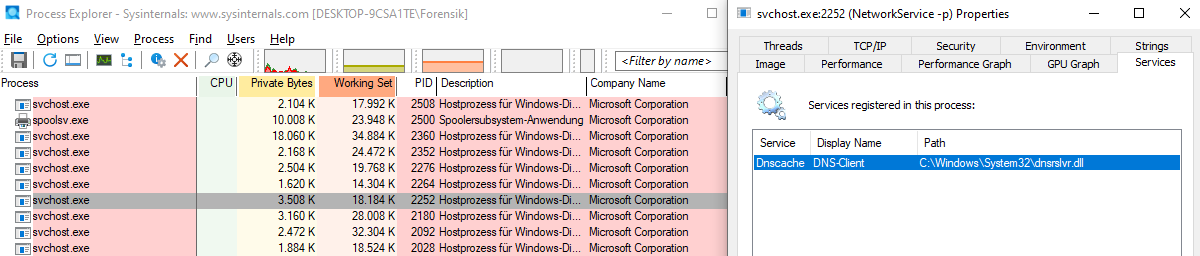
\includegraphics{bilder/firefox-dnscache.png}}}
	\caption{Firefox: Unter dem SVChost-Prozess PID $2252$ läuft der DNSCache-Dienst.}
	\label{chart:svchost-dnscache}  
\end{figure}
Der DNSCache-Dienst unter Windows ist ein Teil des Betriebssystems, der für die Übersetzung von Domainnamen in IP-Adressen verantwortlich ist. Der DNSCache-Dienst speichert DNS-Anfragen und Antworten temporär, um wiederholte DNS-Anfragen zu beschleunigen. \cite{MicrosoftLearn.05.06.2023}
Nach Löschen des DNSCaches mit dem Kommandozeilenbefehl \texttt{ipconfig /flushdns}, dem Schließen aller Process Monitor Instanzen sowie Beenden des DNSCaches Services wurde erneut ein RAM-Dump durchgeführt. Dort wurden keine URL Artefakte mehr gefunden.

\paragraph*{Yara-Regel \glqq{}E-Mail\grqq{}}

\begin{table}[h!]
	\resizebox{\linewidth}{!}{
	\begin{tabular}{r}	
		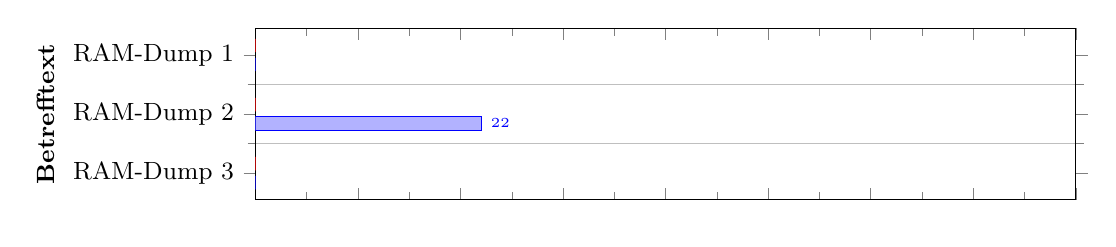
\begin{tikzpicture}
			\begin{axis}[
			xbar,
			width=12cm, 
			height=3cm, 
			ylabel style={align=center}, ylabel=\textbf{Betrefftext},
			y=0.75cm,
			symbolic y coords={RAM-Dump 3, RAM-Dump 2, RAM-Dump 1},
			label style={font=\small},
			tick label style={font=\small},
			ytick=data,
			xticklabels={,,},
            xmin = 0,
            xmax = 80,
			nodes near coords, 
			nodes near coords align={horizontal},
			nodes near coords style={font=\tiny},
   			nodes near coords={\pgfmathfloatifflags{\pgfplotspointmeta}{0}{}{\pgfmathprintnumber{\pgfplotspointmeta}}},
			bar width=.17cm,
			enlarge y limits={abs=2*\pgfplotbarwidth},
			scaled x ticks=false,
			legend style={
				at={(0.5,-0.1)},
				anchor=north
			},
			legend columns=3,
    		yminorgrids = true,minor tick num=1
			]
				\addplot coordinates {
				(0,RAM-Dump 3) (22,RAM-Dump 2) (0,RAM-Dump 1)
				};
				\addplot coordinates {
				(0,RAM-Dump 3) (0,RAM-Dump 2) (0,RAM-Dump 1)
				};
%				\legend{firefox.exe, Andere Prozesse}
			\end{axis}
		\end{tikzpicture}
		\\[-7pt]
		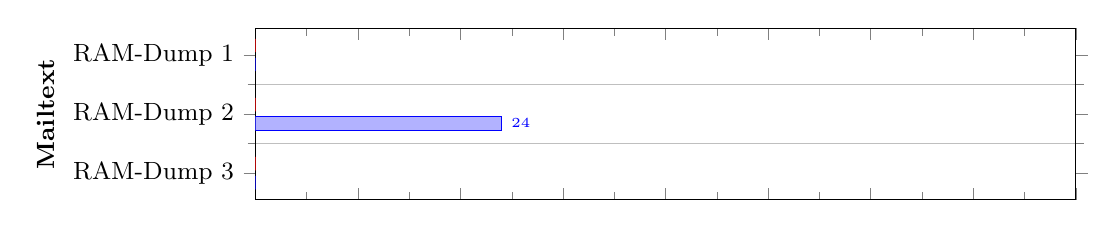
\begin{tikzpicture}
			\begin{axis}[
			xbar,
			width=12cm, 
			height=3cm, 
			ylabel style={align=center}, ylabel=\textbf{Mailtext},
			y=0.75cm,
			symbolic y coords={RAM-Dump 3, RAM-Dump 2, RAM-Dump 1},
			label style={font=\small},
			tick label style={font=\small},
			ytick=data,
			xticklabels={,,},
            xmin = 0,
            xmax = 80,
			nodes near coords, 
			nodes near coords align={horizontal},
			nodes near coords style={font=\tiny},
   			nodes near coords={\pgfmathfloatifflags{\pgfplotspointmeta}{0}{}{\pgfmathprintnumber{\pgfplotspointmeta}}},
			bar width=.17cm,
			enlarge y limits={abs=2*\pgfplotbarwidth},
			scaled x ticks=false,
			legend style={
				at={(0.5,-0.1)},
				anchor=north
			},
			legend columns=3,
    		yminorgrids = true,minor tick num=1
			]
				\addplot coordinates {
				(0,RAM-Dump 3) (24,RAM-Dump 2) (0,RAM-Dump 1)
				};
				\addplot coordinates {
				(0,RAM-Dump 3) (0,RAM-Dump 2) (0,RAM-Dump 1)
				};
%				\legend{firefox.exe, Andere Prozesse}
			\end{axis}
		\end{tikzpicture}	
		\\[-7pt]
		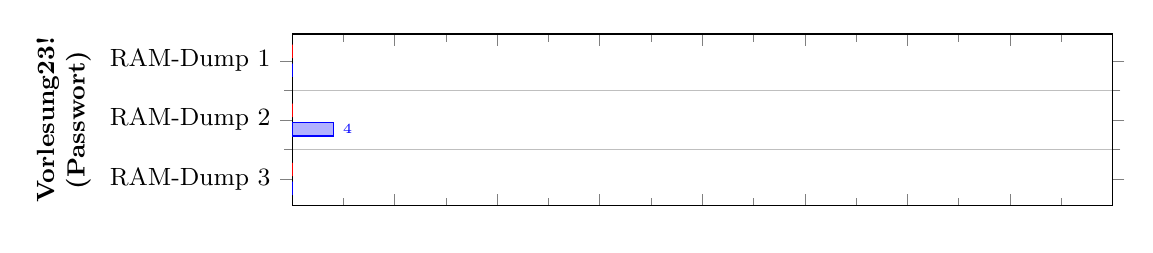
\begin{tikzpicture}
			\begin{axis}[
			xbar,
			width=12cm, 
			height=3cm, 
			ylabel style={align=center}, ylabel=\textbf{Vorlesung23!}\\\textbf{(Passwort)},
			y=0.75cm,
			symbolic y coords={RAM-Dump 3, RAM-Dump 2, RAM-Dump 1},
			label style={font=\small},
			tick label style={font=\small},
			ytick=data,
			xticklabels={,,},
            xmin = 0,
            xmax = 80,
			nodes near coords, 
			nodes near coords align={horizontal},
			nodes near coords style={font=\tiny},
   			nodes near coords={\pgfmathfloatifflags{\pgfplotspointmeta}{0}{}{\pgfmathprintnumber{\pgfplotspointmeta}}},
			bar width=.17cm,
			enlarge y limits={abs=2*\pgfplotbarwidth},
			scaled x ticks=false,
			legend style={
				at={(0.5,-0.1)},
				anchor=north
			},
			legend columns=3,
    		yminorgrids = true,minor tick num=1
			]
				\addplot coordinates {
				(0,RAM-Dump 3) (4,RAM-Dump 2) (0,RAM-Dump 1)
				};
				\addplot coordinates {
				(0,RAM-Dump 3) (0,RAM-Dump 2) (0,RAM-Dump 1)
				};
%				\legend{firefox.exe, Andere Prozesse}
			\end{axis}
		\end{tikzpicture}
		\\[-7pt]
		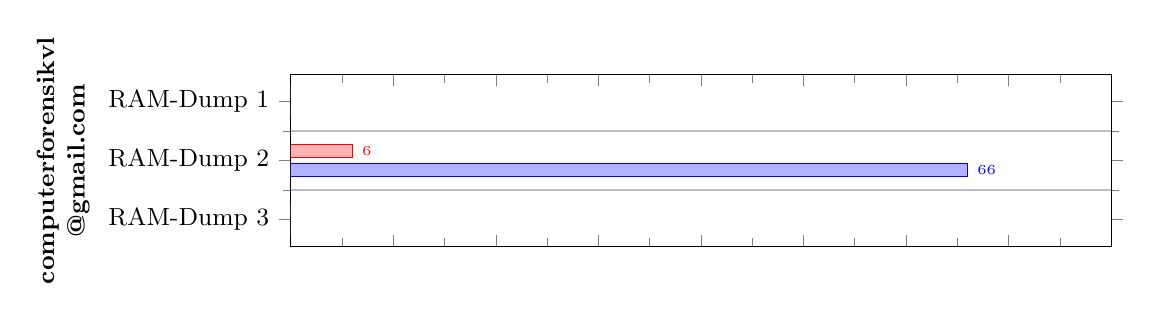
\begin{tikzpicture}
			\begin{axis}[
			xbar,
			width=12cm, 
			height=3cm, 
			ylabel style={align=center}, ylabel=\textbf{computerforensikvl}\\\textbf{@gmail.com},
			y=0.75cm,
			symbolic y coords={RAM-Dump 3, RAM-Dump 2, RAM-Dump 1},
			label style={font=\small},
			tick label style={font=\small},
			ytick=data,
			xticklabels={,,},
            xmin = 0,
            xmax = 80,
			nodes near coords, 
			nodes near coords align={horizontal},
			nodes near coords style={font=\tiny},
   			nodes near coords={\pgfmathfloatifflags{\pgfplotspointmeta}{0}{}{\pgfmathprintnumber{\pgfplotspointmeta}}},
			bar width=.17cm,
			enlarge y limits={abs=2*\pgfplotbarwidth},
			scaled x ticks=false,
			legend style={
				at={(0.5,-0.1)},
				anchor=north
			},
			legend columns=3,
    		yminorgrids = true,minor tick num=1
			]
				\addplot coordinates {
				(0,RAM-Dump 3) (66,RAM-Dump 2) (0,RAM-Dump 1)
				};
				\addplot coordinates {
				(0,RAM-Dump 3) (6,RAM-Dump 2) (0,RAM-Dump 1)
				};
%				\legend{firefox.exe, Andere Prozesse}
			\end{axis}
		\end{tikzpicture}	
		\\[-7pt]
		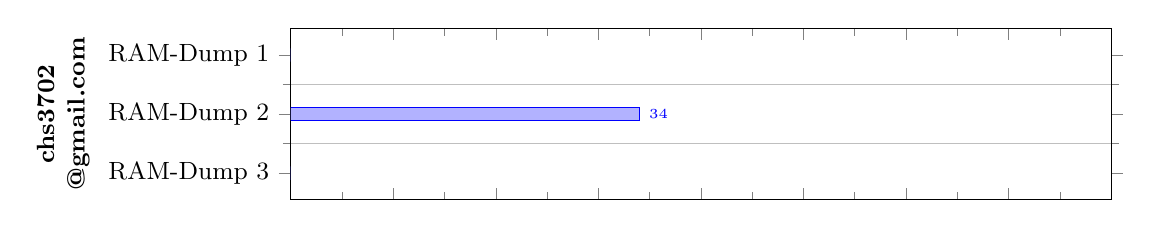
\begin{tikzpicture}
			\begin{axis}[
			xbar,
			width=12cm, 
			height=3cm, 
			ylabel style={align=center}, ylabel=\textbf{chs3702}\\\textbf{@gmail.com},
			y=0.75cm,
			symbolic y coords={RAM-Dump 3, RAM-Dump 2, RAM-Dump 1},
			label style={font=\small},
			tick label style={font=\small},
			ytick=data,
			xticklabels={,,},
            xmin = 0,
            xmax = 80,
			nodes near coords, 
			nodes near coords align={horizontal},
			nodes near coords style={font=\tiny},
   			nodes near coords={\pgfmathfloatifflags{\pgfplotspointmeta}{0}{}{\pgfmathprintnumber{\pgfplotspointmeta}}},
			bar width=.17cm,
			enlarge y limits={abs=2*\pgfplotbarwidth},
			scaled x ticks=false,
			legend style={
				at={(0.5,-0.1)},
				anchor=north
			},
			legend columns=3,
    		yminorgrids = true,minor tick num=1
			]
				\addplot coordinates {
				(0,RAM-Dump 3) (34,RAM-Dump 2) (0,RAM-Dump 1)
				};
%				\legend{firefox.exe, Andere Prozesse}
			\end{axis}
		\end{tikzpicture}
		\\[-7pt]
		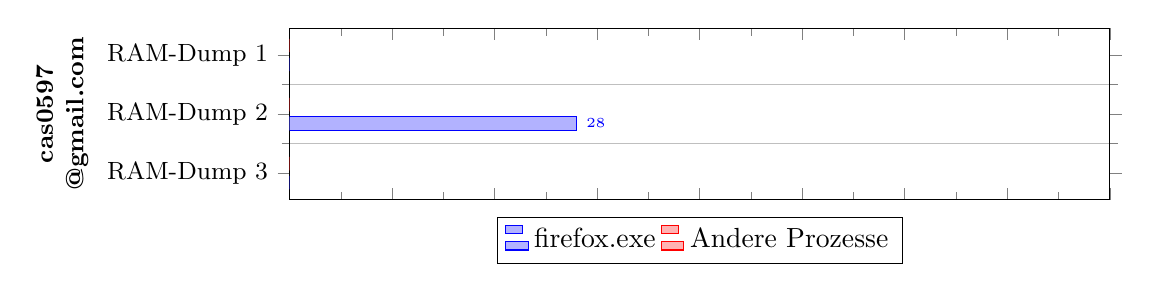
\begin{tikzpicture}
			\begin{axis}[
			xbar,
			width=12cm, 
			height=3cm, 
			ylabel style={align=center}, ylabel=\textbf{cas0597}\\\textbf{@gmail.com},
			y=0.75cm,
			symbolic y coords={RAM-Dump 3, RAM-Dump 2, RAM-Dump 1},
			label style={font=\small},
			tick label style={font=\small},
			ytick=data,
			xticklabels={,,},
            xmin = 0,
            xmax = 80,
			nodes near coords, 
			nodes near coords align={horizontal},
			nodes near coords style={font=\tiny},
   			nodes near coords={\pgfmathfloatifflags{\pgfplotspointmeta}{0}{}{\pgfmathprintnumber{\pgfplotspointmeta}}},
			bar width=.17cm,
			enlarge y limits={abs=2*\pgfplotbarwidth},
			scaled x ticks=false,
			legend style={
				at={(0.5,-0.1)},
				anchor=north
			},
			legend columns=3,
    		yminorgrids = true,minor tick num=1
			]
				\addplot coordinates {
				(0,RAM-Dump 3) (28,RAM-Dump 2) (0,RAM-Dump 1)
				};
				\addplot coordinates {
				(0,RAM-Dump 3) (0,RAM-Dump 2) (0,RAM-Dump 1)
				};
				\legend{firefox.exe, Andere Prozesse}
			\end{axis}
		\end{tikzpicture}
				%	\begin{axis}[]
		%	\legend{Logfile 1, Logfile 2}
		%	\end{axis}

	\end{tabular}
	}
	\captionof{figure}{Firefox: Anzahl gefundener E-Mail Artefakte im RAM}
	\label{chart:firefox-volatility-mail}
\end{table}

%\begin{figure}[h!]
%	\centerline{\resizebox{\linewidth}{!}{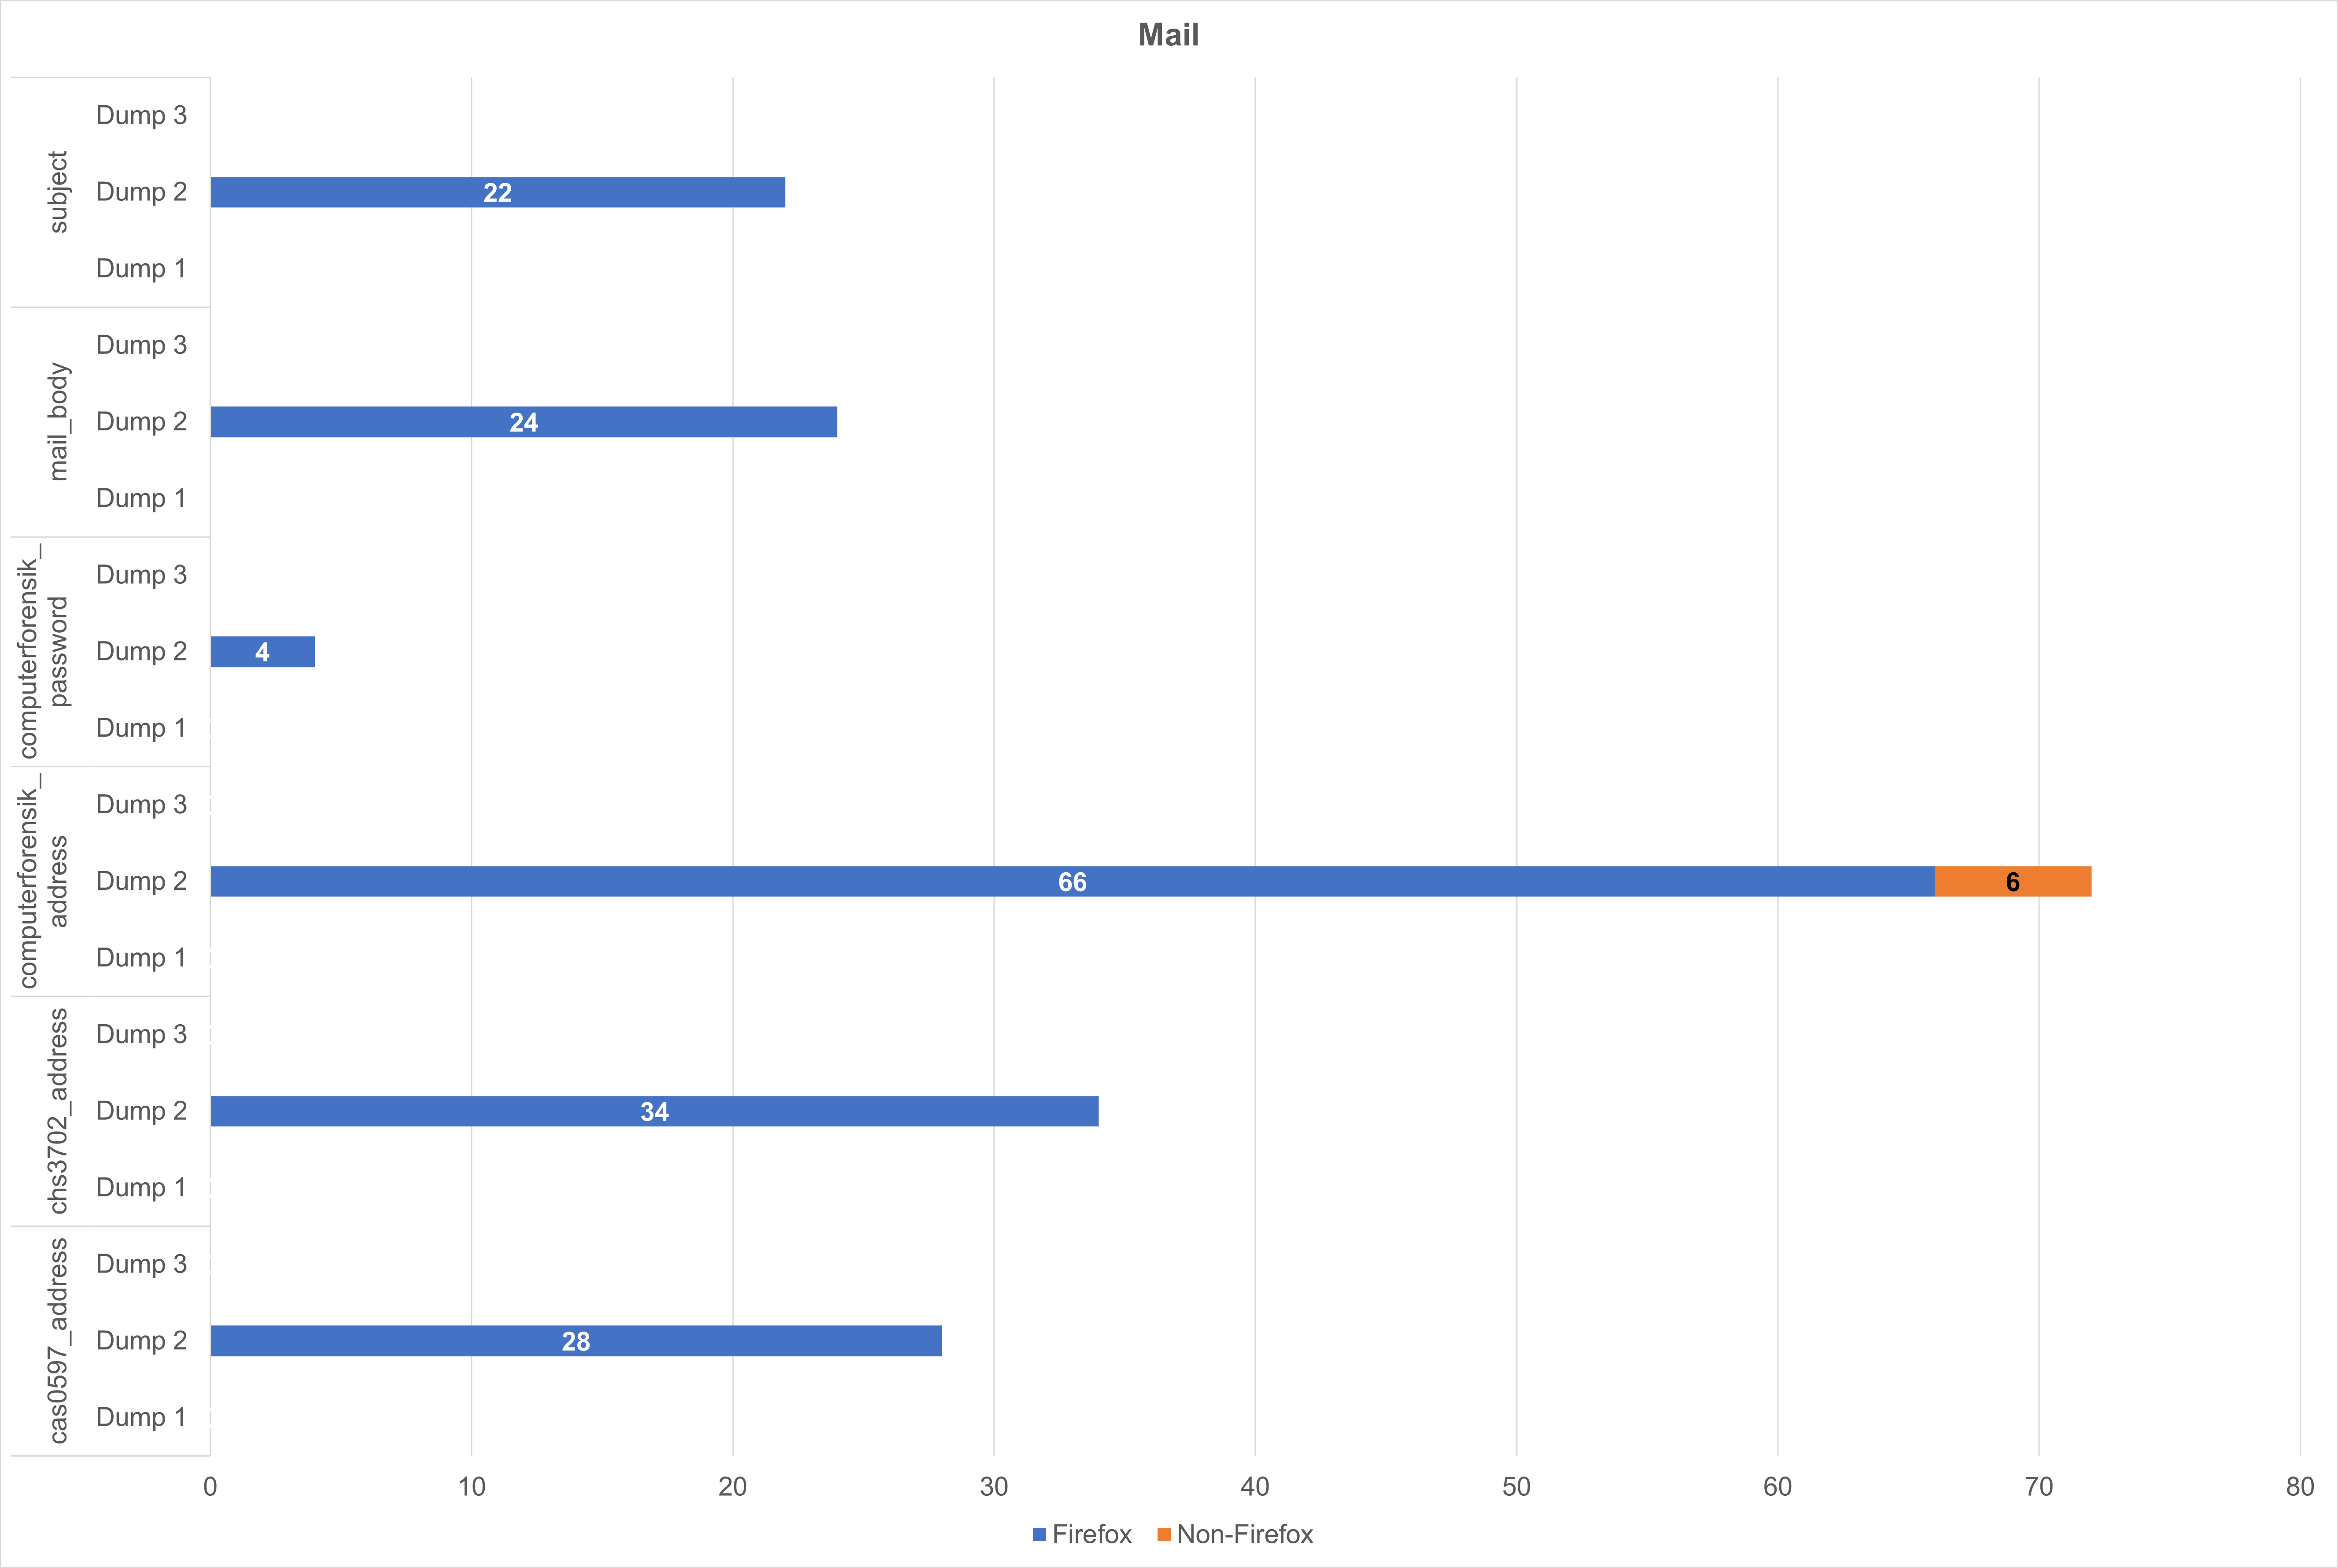
\includegraphics{bilder/volatility/firefox/mail.png}}}
%	\label{chart:final-criteria}  
%	\caption{Mail}
%\end{figure}
Wie in Abbildung \ref{chart:firefox-volatility-mail} gezeigt, wurden E-Mail-Artefakte ausschließlich nach dem Browsing-Szenario mit geöffnetem Firefox Browser (RAM-Dump 2) gefunden. Dabei wurden Artefakte jeder Kategorie gefunden.
Unter den gefundenen Artefakten befindet sich am häufigsten die Absenderadresse \glqq{}computerforensikvl@gmail.com\grqq{}. Dieses Artefakt wurde als einziges E-Mail-Artefakt sechsmal in anderen Prozessen als Firefox gefunden.

Bemerkenswert ist, dass das Passwort des Google-Accounts, mit dem die E-Mails verschickt wurden, viermal als Klartext im RAM gefunden wurden. Das Passwort wurde je zweimal in zwei Firefox Prozessen mit den PIDs 7420 und 8424 gefunden. Tabelle \ref{tab:firefox-mapping-virtaddr-to-byteoffset} zeigt die virtuellen Speicheradressen der Artefakte aus der Yarascan Ausgabe.
\begin{table}[h!]
\caption{Firefox: Abbildung der virtellen Speicheradressen der gefundenen Strings auf Byte-Offsets der entsprechenden Speicherseiten}
\label{tab:firefox-mapping-virtaddr-to-byteoffset}
\resizebox{\linewidth}{!}{
\begin{tabular}{|c|c|c|ll}
\cline{1-3}
\textbf{Virtuelle Speicheradresse} & \textbf{PID} & \textbf{Byte-Offset in extrahierter Speicherseite} &  &  \\ \cline{1-3}
0xb9ce29180c8                      & 7420         & 0x11dd40c8                                         &  &  \\ \cline{1-3}
0x2859f4ffd4e0                     & 7420         & 0x12e234e0                                         &  &  \\ \cline{1-3}
0x24083b41858                      & 8424         & 0x583858                                           &  &  \\ \cline{1-3}
0x240840e5b08                      & 8424         & 0x96bb08                                           &  &  \\ \cline{1-3}
\end{tabular}
}
\end{table}

Zu diesen Artefakten wurde gemäß Methodik in Abschnitt \ref{subsubsection:ergebnisse-firefox-uncommonlocations-analysemitvolatility} der String Kontext -- also die Zeichen vor und nach dem gefundenen Artefakt im Speicherbereich -- ermittelt. Dazu wurde mithilfe des Volatility memmap Plugins die Abbildung der virtuellen Speicheradressen auf den Byte-Offset in der extrahierten Speicherseite des Prozesses ermittelt. 

\begin{figure}[h!]
	\centering
	\subcaptionbox{Byte-Offset 0x11dd40c8}{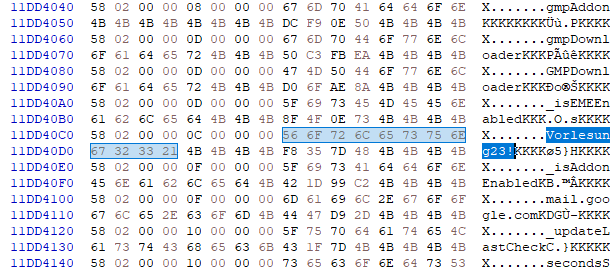
\includegraphics[width=0.47\textwidth]{bilder/volatility/firefox/password_0xb9ce29180c8_7420.png}}%
	\hfill
	\subcaptionbox{Byte-Offset 0x12e234e0}{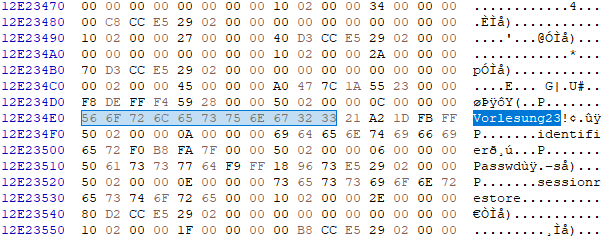
\includegraphics[width=0.47\textwidth]{bilder/volatility/firefox/password_0x2859f4ffd4e0_7420.png}}%
	\caption{Firefox: Passwort-Klartext in Speicherseiten von PID 7420}
	\label{img:firefox-pw-offset-pid-7420}  
\end{figure}
Wie in Abbildung \ref{img:firefox-pw-offset-pid-7420} gezeigt, sind in der Speicherseite des Prozesses mit PID 7420 in unmittelbarer Umgebung des gefundenen Passworts am Byte-Offset 0xb9ce29180c8 Code-Fragmente der \textit{Gecko-Engine} zu finden. Dieser Teil des Firefox Browsers ist für das Rendering von Webinhalten verantwortlich, einschließlich HTML, CSS, JavaScript und anderen Medienformaten wie Bildern, Audio und Video. \cite{MozillaWiki.05.06.2023}
In der gleichen Datei konnten nach dem gefundenen Passwort am Byte-Offset $0x12e234e0$ die Strings \glqq{}Passwd\grqq{} sowie \glqq{}sessionrestore\grqq{} (siehe Common Location \textit{Sessionstore} in Anhang \ref{subsubsection:appendix-firefox-common-locations-writefile-operations}) identifiziert werden. 

\begin{figure}[h!]
	\centering
	\subcaptionbox{Byte-Offset 0x583858}{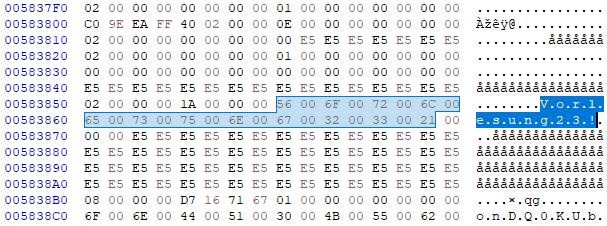
\includegraphics[width=0.47\textwidth]{bilder/volatility/firefox/password_0x24083b41858_8424.png}}%
	\hfill
	\subcaptionbox{Byte-Offset 0x96bb08}{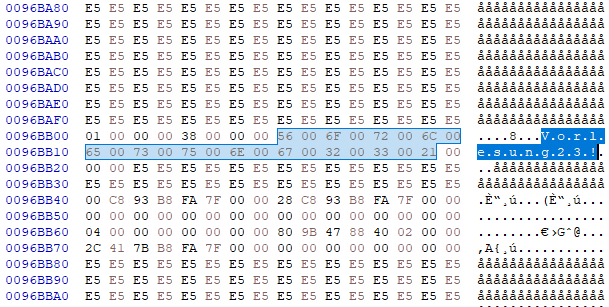
\includegraphics[width=0.47\textwidth]{bilder/volatility/firefox/password_0x240840e5b08_8424.png}}%
	\caption{Firefox: Passwort-Klartext in Speicherseiten von PID 8424}
	\label{img:firefox-pw-offset-pid-8424}  
\end{figure}
Wie in Abbildung \ref{img:firefox-pw-offset-pid-8424} gezeigt, kann in den Byte-Offsets der gefundenen Passwörter in der Speicherseite der PID 8424 kein sinnvoller Kontext ermittelt werden. Im Gegensatz zur Speicherseite der PID 7420 wird das Passwort dort mit 2 Bytes pro Zeichen enkodiert, was eine Unicode-Zeichenenkodierung vermuten lässt.

\paragraph*{Yara-Regel \glqq{}DK-Logo\grqq{}}
Wie in Abbildung \ref{chart:firefox-volatility-image} gezeigt, wurde das im Browsing-Szenario geöffnete Donaukurier Logo ausschließlich im zweiten RAM-Dump dreimal in Firefox Prozessen gefunden.
\begin{table}[h!]
	\resizebox{\linewidth}{!}{
	\begin{tabular}{r}
		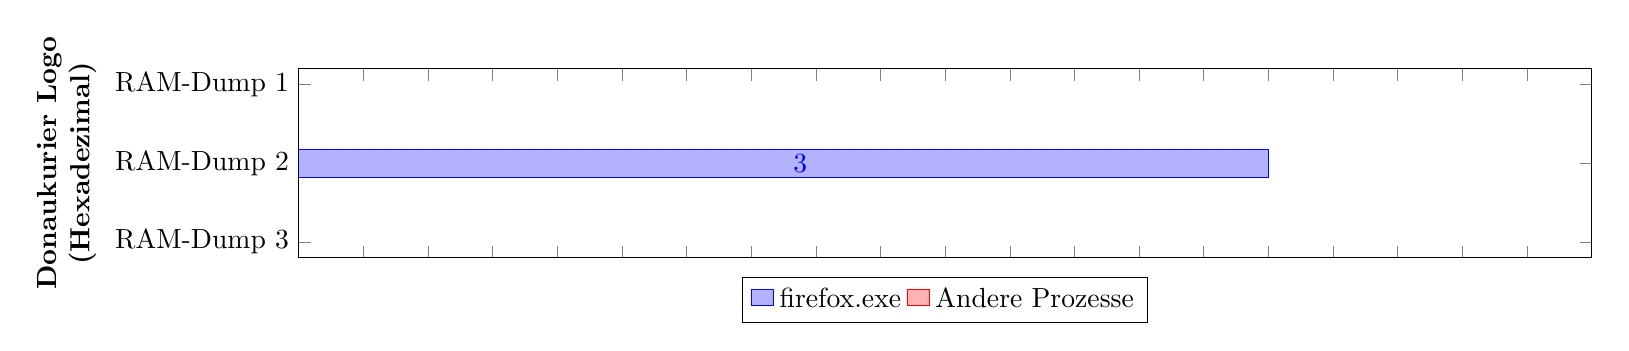
\begin{tikzpicture}
			\begin{axis}[
			xbar stacked,
			width=18cm, 
			height=12cm, 
			ylabel style={align=center}, ylabel=\textbf{Donaukurier Logo}\\\textbf{(Hexadezimal)},
			y=1cm,
			symbolic y coords={RAM-Dump 3, RAM-Dump 2, RAM-Dump 1},
			ytick=data,
			xticklabels={,,},
            xmin = 0,
            xmax = 4,
			nodes near coords, 
			nodes near coords align={horizontal},
			legend style={
				at={(0.5,-0.1)},
				anchor=north
			},
			legend columns=2
			]
				\addplot coordinates {
				(0,RAM-Dump 3) (3,RAM-Dump 2) (0,RAM-Dump 1)
				};
				\addplot coordinates {
				(0,RAM-Dump 3) (0,RAM-Dump 2) (0,RAM-Dump 1)
				};
				\legend{firefox.exe, Andere Prozesse}
			\end{axis}
		\end{tikzpicture}
	\end{tabular}
	}
	\captionof{figure}{Firefox: Anzahl gefundener Hexadezimalwerte des Donaukurier-Logos im RAM}
	\label{chart:firefox-volatility-image}
\end{table}
%\begin{figure}[h!]
%	\centerline{\resizebox{\linewidth}{!}{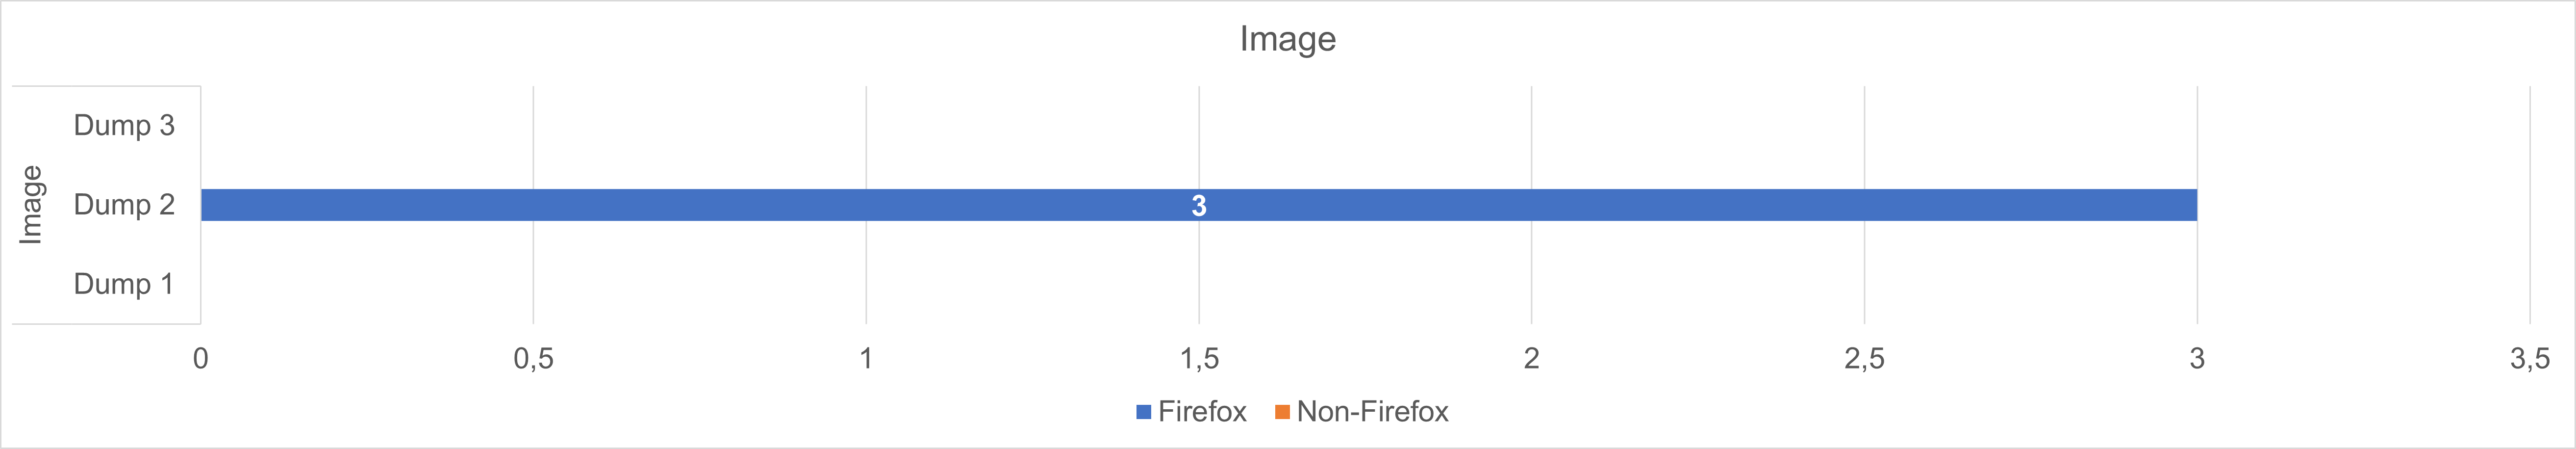
\includegraphics{bilder/volatility/firefox/image.png}}}
%	\label{chart:final-criteria}  
%	\caption{Image}
%\end{figure}



%\begin{figure}[h!]
%	\centerline{\resizebox{\linewidth}{!}{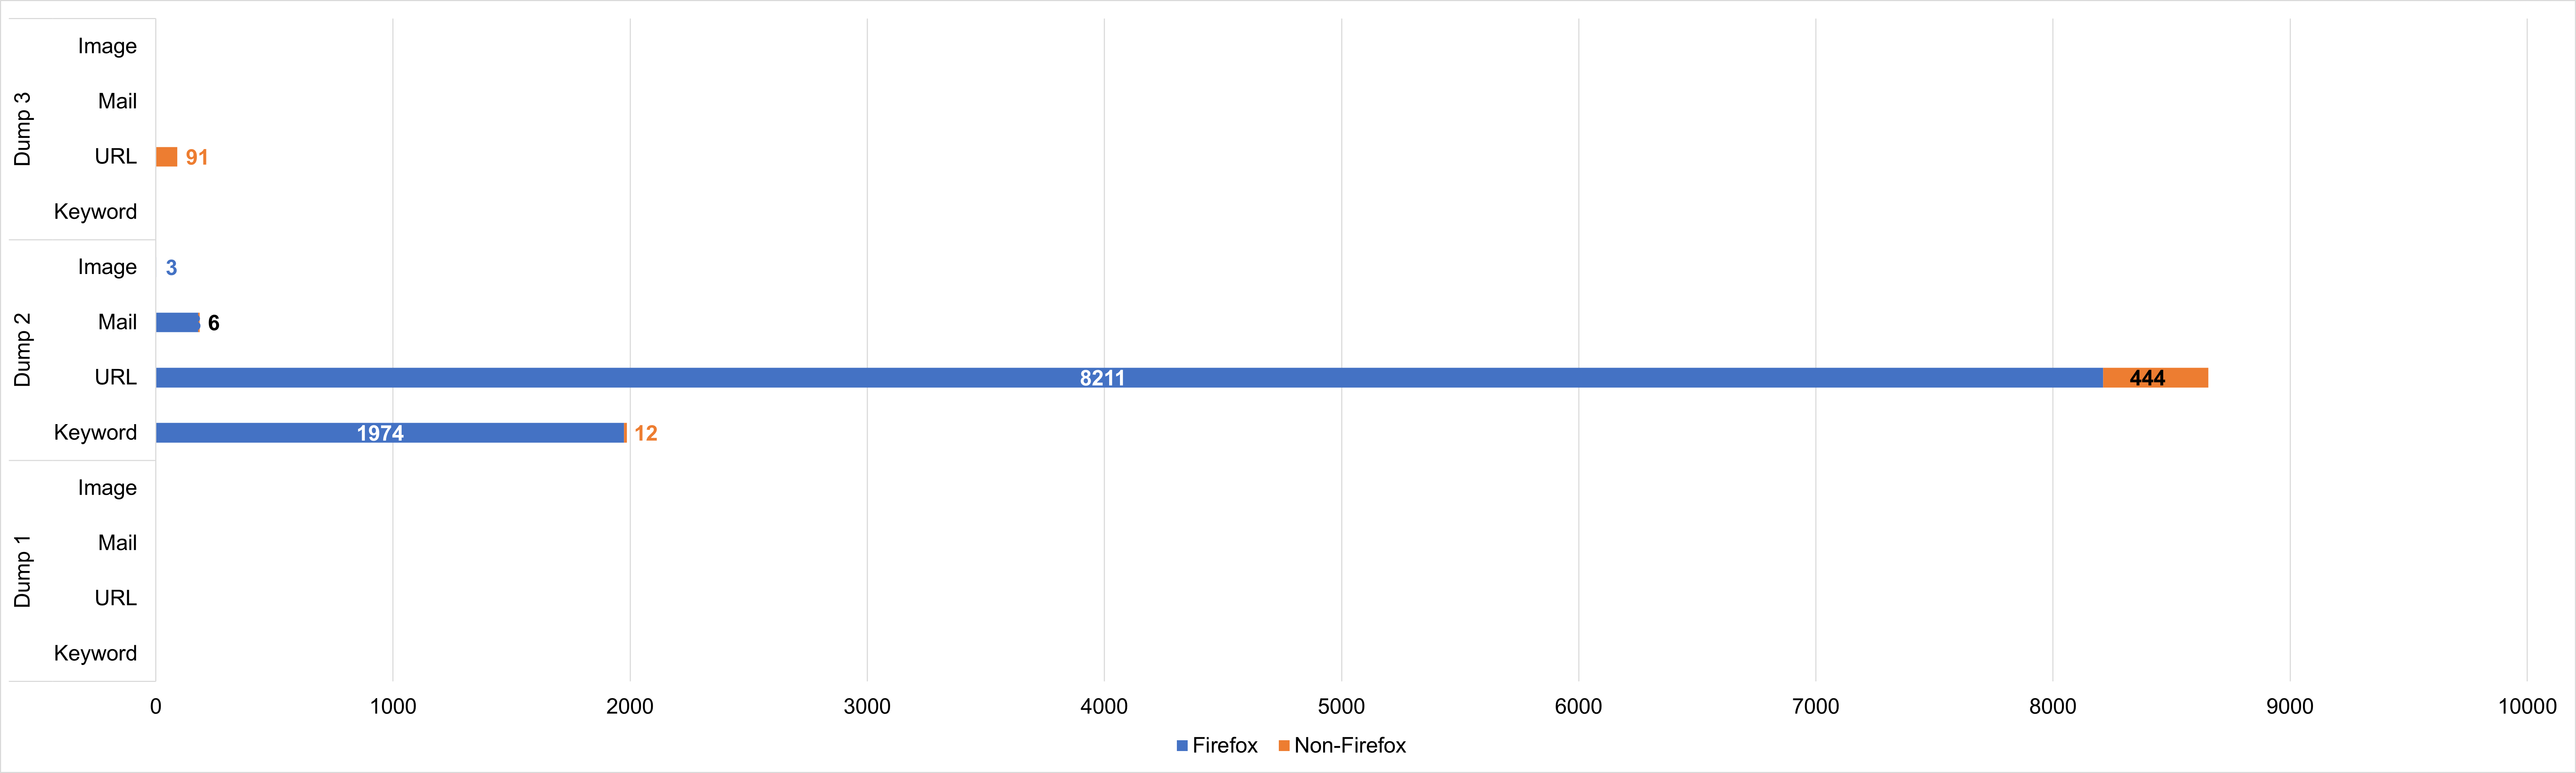
\includegraphics{bilder/volatility/firefox/summary.png}}}
%	\label{chart:final-criteria}  
%	\caption{Summary}
%\end{figure}

\subsection*{Registry}
\label{subsection:ergebnisse-firefox-registry}
Die Analyse der Registry zählt gemäß Methodik in Abschnitt \ref{subsection:methodik-datenanalyse-registry} sowohl zu den Common als auch Uncommon Locations. Weder in den Process Monitor \glqq{}SetValue\grqq{} Operations noch in den System- und User-Hives konnten PB-Artefakte gefunden werden. Eine detaillierte Analyse dieser Common- und Uncommon Locations der Registry ist im Anhang \ref{subsection:appendix-firefox-registry} beschrieben.


%*** TODO: Zusammenfassung Firefox ***


\newpage


% ######################################################################
% ######################################################################
% ######################################################################
% ######################################################################


\section{Tor-Browser}\label{section:ergebnisse-tor}

In diesem Abschnitt werden die Ergebnisse der Datenanalyse der Common Locations, Uncommon Locations sowie der Registry für den Tor-Browser präsentiert.

\subsection*{Common Locations}
Zunächst werden die Common Locations analysiert, um potenzielle Hinweise auf Internetaktivitäten des Browsing-Szenarios zu finden. Bei der Untersuchung der gängigen Speicherorte wurde gemäß der im Abschnitt \ref{subsection:methodik-datenanalyse-commonlocations} beschriebenen Methodik zwischen Schreibvorgängen in den Logdateien des Process Monitors und den SQLite-Datenbanken zur Verwaltung von Benutzerdaten unterschieden. Dabei konnten in keiner Datei PB-Artefakte gefunden werden. Eine detaillierte Analyse der Process Monitor \glqq{}WriteFile\grqq{} Operations sowie der SQLite-Datenbanken ist im Anhang \ref{subsection:appendix-tor-common-locations} beschrieben.

\subsection*{Uncommon Locations}
Nachfolgend werden die Analyseergebnisse der Tor Uncommon Locations beschrieben.
Dazu werden die vollständigen Speicherabbilder nach PB-Artefakten untersucht, ohne das genaue Browserverhalten zu berücksichtigen. Stattdessen wird sich auf die Vollständigkeit der Funktionen der Forensik-Tools Autopsy und Volatility verlassen.

\subsubsection*{Analyse mit Autopsy}
Autopsy wird bei den Uncommon Locations als konkretes forensisches Werkzeug verwendet, statt nur zur Dateiextraktion, wie es bei den Common Locations der Fall war.

Eine Stichwortsuche nach PB-Artefakten in Autopsy in allen fünf Tor Festplatten-Images ergab keine Treffer.

Ebenso wurden in den automatisch von Autopsy kategorisierten Dateien keine PB-Artefakte gefunden. 
Im Anhang \ref{subsubsection:appendix-tor-uncommon-locations-autopsy} ist eine detaillierte Analyse der kategorisierten Dateien beschrieben.


\subsubsection*{Analyse mit Volatility}
Bei der Untersuchung der Tor RAM-Dumps mithilfe des Volatility Plugins Yarascan, konnten PB-Artefakte identifiziert werden.
Nachfolgend werden die Ergebnisse geordnet nach Yara-Regeln beschrieben. Die vollständigen Yara-Regeln sind im Anhang \ref{appendix:yara-regeln} aufgelistet.

\paragraph*{Yara-Regel \glqq{}HTML\grqq{}}
Wie bei Firefox, konnten keine HTML-Artefakte im RAM gefunden werden. Deshalb wird diese Kategorie nicht weiter aufgeführt.

\paragraph*{Yara-Regel \glqq{}Suchbegriffe\grqq{}}
Wie in Abbildung \ref{chart:tor-volatility-keywords} gezeigt, wurden nach dem Browsing-Szenarios sowie vor (RAM-Dump 2) als auch nach Erstellen einer \glqq{}Neuen Identität\grqq{} (RAM-Dump 3-1) Suchbegriffe des Browsing-Szenarios gefunden.
Nachdem eine \glqq{}Neue Identität\grqq{} erstellt wurde, reduzierten sich die gefundenen Artefakte deutlich. 
Die Suchbegriffe wurden hauptsächlich in Firefox-Prozessen gefunden. Kein Artefakt war im Tor-Prozess zu finden.
Mit 4833 Artefakten wurde am häufigsten der Suchbegriff \glqq{}pfaffenhofen\grqq{} nach dem Browsing-Szenario im zweiten RAM-Dump gefunden. 
Nach dem Schließen des Tor-Browsers wurden keine Suchbegriffe im RAM identifiziert.

\begin{table}[h!]
	\resizebox{\linewidth}{!}{
	\begin{tabular}{l}	
		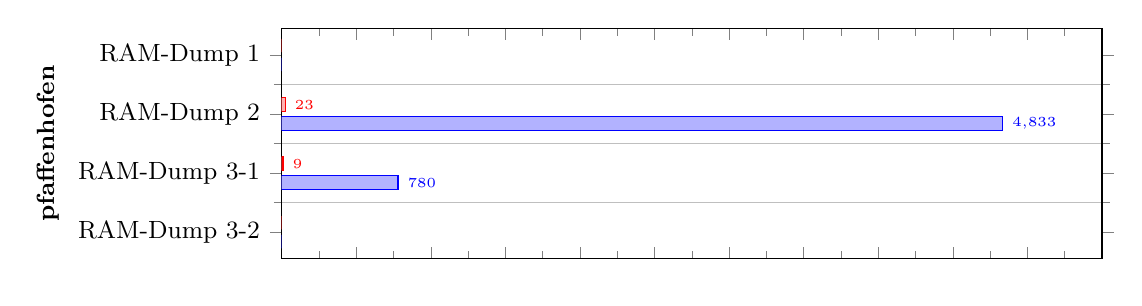
\begin{tikzpicture}
			\begin{axis}[
			xbar,
			width=12cm, 
			height=3cm, 
			ylabel style={align=center}, ylabel=\textbf{pfaffenhofen},
			y=0.75cm,
			symbolic y coords={RAM-Dump 3-2, RAM-Dump 3-1, RAM-Dump 2, RAM-Dump 1},
			label style={font=\small},
			tick label style={font=\small},
			ytick=data,
			xticklabels={,,},
            xmin = 0,
            xmax = 5500,
			nodes near coords, 
			nodes near coords align={horizontal},
			nodes near coords style={font=\tiny},
   			nodes near coords={\pgfmathfloatifflags{\pgfplotspointmeta}{0}{}{\pgfmathprintnumber{\pgfplotspointmeta}}},
			bar width=.17cm,
			enlarge y limits={abs=2*\pgfplotbarwidth},
			scaled x ticks=false,
			legend style={
				at={(0.5,-0.1)},
				anchor=north
			},
			legend columns=3,
    		yminorgrids = true,minor tick num=1
			]
				\addplot coordinates {
				(0,RAM-Dump 3-2)  (780,RAM-Dump 3-1) (4833,RAM-Dump 2) (0,RAM-Dump 1)
				};
%				\addplot coordinates {
%				(0,RAM-Dump 3-2)  (0,RAM-Dump 3-1) (0,RAM-Dump 2) (0,RAM-Dump 1)
%				};
				\addplot coordinates {
				(0,RAM-Dump 3-2)  (9,RAM-Dump 3-1) (23,RAM-Dump 2) (0,RAM-Dump 1)
				};
%				\legend{firefox.exe, tor.exe, Andere Prozesse}
			\end{axis}
		\end{tikzpicture}
		\\[-7pt]
		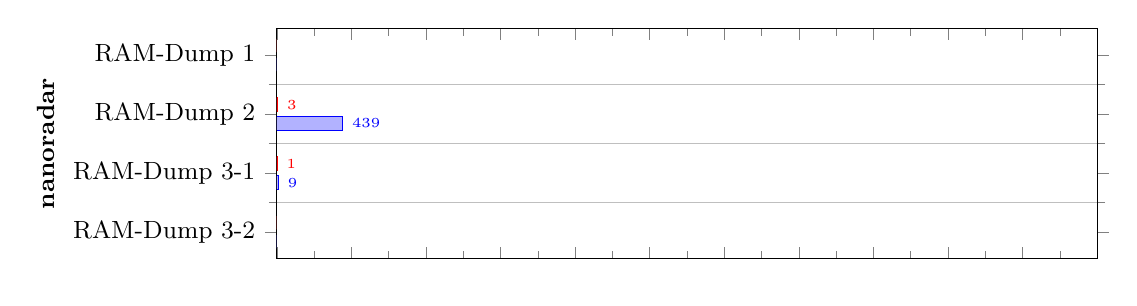
\begin{tikzpicture}
			\begin{axis}[
			xbar,
			width=12cm, 
			height=3cm, 
			ylabel style={align=center}, ylabel=\textbf{nanoradar},
			y=0.75cm,
			symbolic y coords={RAM-Dump 3-2, RAM-Dump 3-1, RAM-Dump 2, RAM-Dump 1},
			label style={font=\small},
			tick label style={font=\small},
			ytick=data,
			xticklabels={,,},
            xmin = 0,
            xmax = 5500,
			nodes near coords, 
			nodes near coords align={horizontal},
			nodes near coords style={font=\tiny},
   			nodes near coords={\pgfmathfloatifflags{\pgfplotspointmeta}{0}{}{\pgfmathprintnumber{\pgfplotspointmeta}}},
			bar width=.17cm,
			enlarge y limits={abs=2*\pgfplotbarwidth},
			scaled x ticks=false,
			legend style={
				at={(0.5,-0.1)},
				anchor=north
			},
			legend columns=3,
    		yminorgrids = true,minor tick num=1
			]
				\addplot coordinates {
				(0,RAM-Dump 3-2)  (9,RAM-Dump 3-1) (439,RAM-Dump 2) (0,RAM-Dump 1)
				};
%				\addplot coordinates {
%				(0,RAM-Dump 3-2)  (0,RAM-Dump 3-1) (0,RAM-Dump 2) (0,RAM-Dump 1)
%				};
				\addplot coordinates {
				(0,RAM-Dump 3-2)  (1,RAM-Dump 3-1) (3,RAM-Dump 2) (0,RAM-Dump 1)
				};
%				\legend{firefox.exe, tor.exe, Andere Prozesse}
			\end{axis}
		\end{tikzpicture}
		\\[-7pt]
		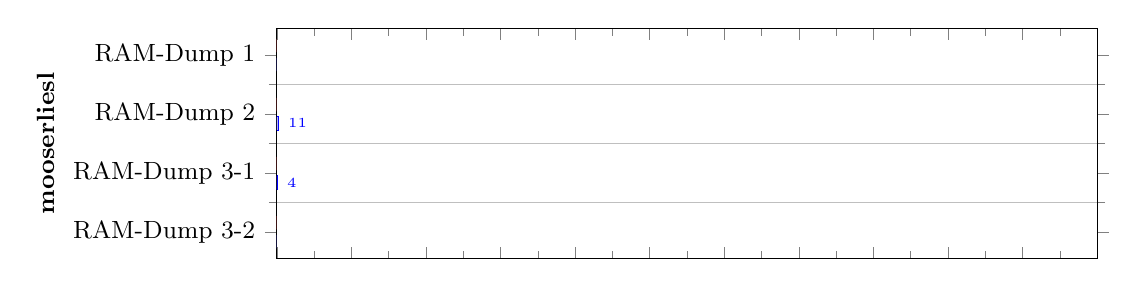
\begin{tikzpicture}
			\begin{axis}[
			xbar,
			width=12cm, 
			height=3cm, 
			ylabel style={align=center}, ylabel=\textbf{mooserliesl},
			y=0.75cm,
			symbolic y coords={RAM-Dump 3-2, RAM-Dump 3-1, RAM-Dump 2, RAM-Dump 1},
			label style={font=\small},
			tick label style={font=\small},
			ytick=data,
			xticklabels={,,},
            xmin = 0,
            xmax = 5500,
			nodes near coords, 
			nodes near coords align={horizontal},
			nodes near coords style={font=\tiny},
   			nodes near coords={\pgfmathfloatifflags{\pgfplotspointmeta}{0}{}{\pgfmathprintnumber{\pgfplotspointmeta}}},
			bar width=.17cm,
			enlarge y limits={abs=2*\pgfplotbarwidth},
			scaled x ticks=false,
			legend style={
				at={(0.5,-0.1)},
				anchor=north
			},
			legend columns=3,
    		yminorgrids = true,minor tick num=1
			]
				\addplot coordinates {
				(0,RAM-Dump 3-2)  (4,RAM-Dump 3-1) (11,RAM-Dump 2) (0,RAM-Dump 1)
				};
%				\addplot coordinates {
%				(0,RAM-Dump 3-2)  (0,RAM-Dump 3-1) (0,RAM-Dump 2) (0,RAM-Dump 1)
%				};
				\addplot coordinates {
				(0,RAM-Dump 3-2)  (0,RAM-Dump 3-1) (0,RAM-Dump 2) (0,RAM-Dump 1)
				};
%				\legend{firefox.exe, tor.exe, Andere Prozesse}
			\end{axis}
		\end{tikzpicture}
		\\[-7pt]
		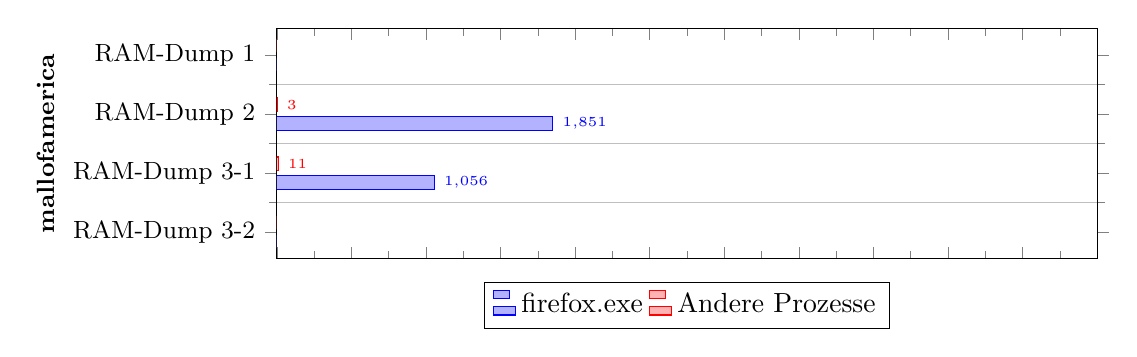
\begin{tikzpicture}
			\begin{axis}[
			xbar,
			width=12cm, 
			height=3cm, 
			ylabel style={align=center}, ylabel=\textbf{mallofamerica},
			y=0.75cm,
			symbolic y coords={RAM-Dump 3-2, RAM-Dump 3-1, RAM-Dump 2, RAM-Dump 1},
			label style={font=\small},
			tick label style={font=\small},
			ytick=data,
			xticklabels={,,},
            xmin = 0,
            xmax = 5500,
			nodes near coords, 
			nodes near coords align={horizontal},
			nodes near coords style={font=\tiny},
   			nodes near coords={\pgfmathfloatifflags{\pgfplotspointmeta}{0}{}{\pgfmathprintnumber{\pgfplotspointmeta}}},
			bar width=.17cm,
			enlarge y limits={abs=2*\pgfplotbarwidth},
			scaled x ticks=false,
			legend style={
				at={(0.5,-0.1)},
				anchor=north
			},
			legend columns=3,
    		yminorgrids = true,minor tick num=1
			]
				\addplot coordinates {
				(0,RAM-Dump 3-2)  (1056,RAM-Dump 3-1) (1851,RAM-Dump 2) (0,RAM-Dump 1)
				};
%				\addplot coordinates {
%				(0,RAM-Dump 3-2)  (0,RAM-Dump 3-1) (0,RAM-Dump 2) (0,RAM-Dump 1)
%				};
				\addplot coordinates {
				(0,RAM-Dump 3-2)  (11,RAM-Dump 3-1) (3,RAM-Dump 2) (0,RAM-Dump 1)
				};
				\legend{firefox.exe, Andere Prozesse}
			\end{axis}
		\end{tikzpicture}
	\end{tabular}
	}
	\captionof{figure}{Tor-Browser: Anzahl gefundenener Suchbegriffe im RAM}
	\label{chart:tor-volatility-keywords}
\end{table}
%\begin{figure}[h!]
%	\centerline{\resizebox{\linewidth}{!}{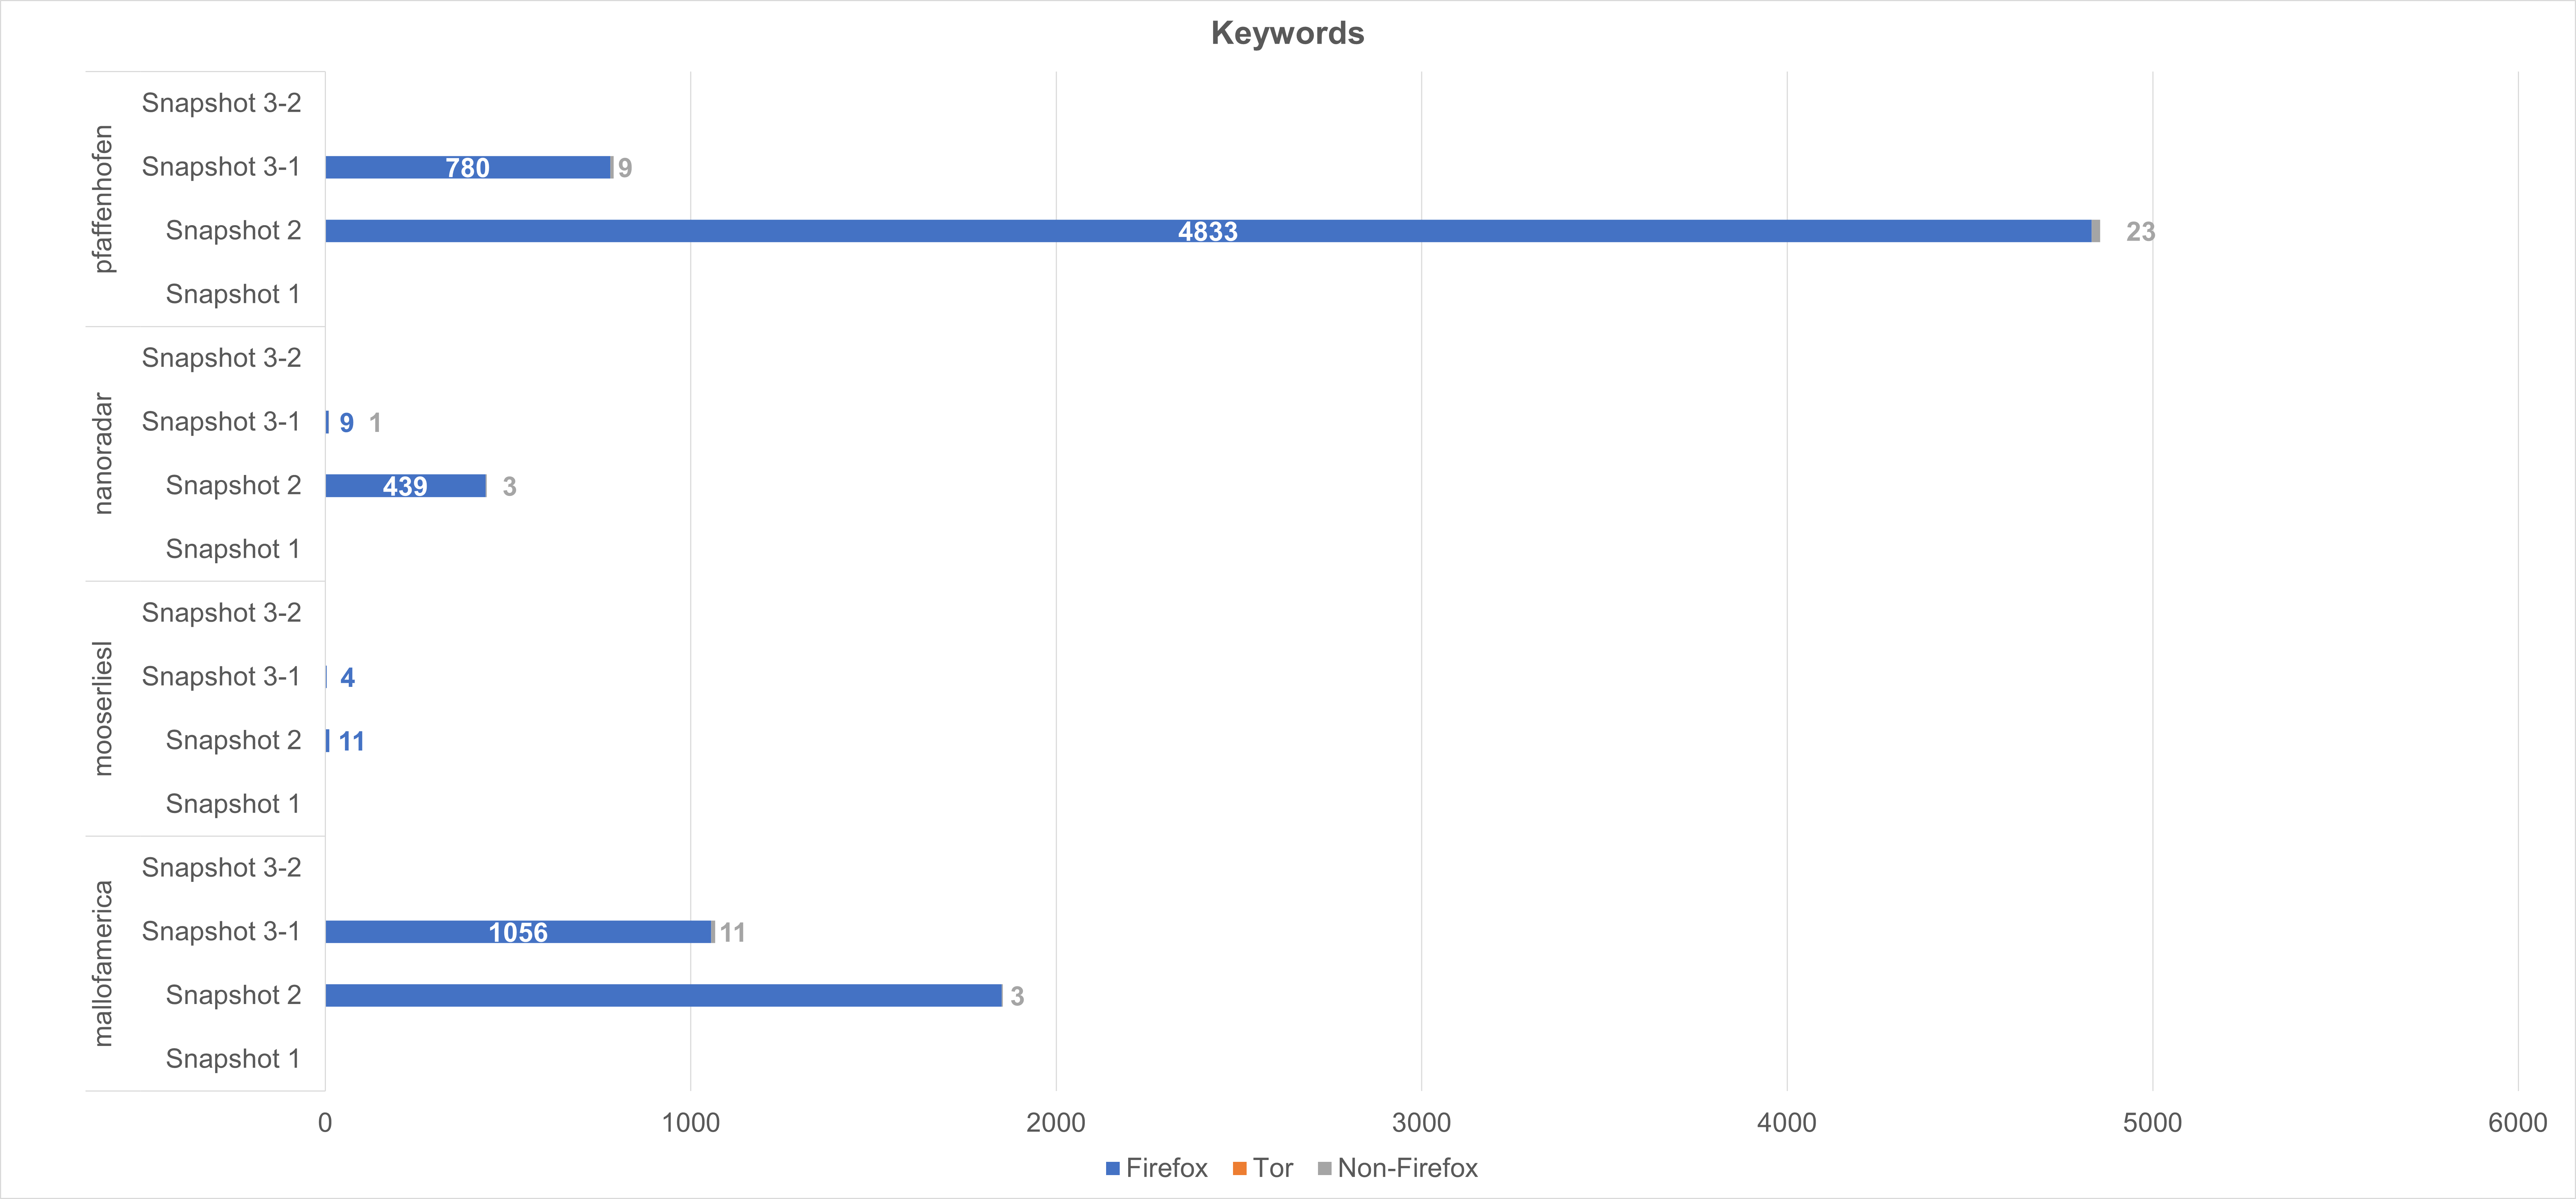
\includegraphics{bilder/volatility/tor/keywords.png}}}
%	\label{chart:final-criteria}  
%	\caption{Keywords}
%\end{figure}

\paragraph*{Yara-Regel \glqq{}URLs\grqq{}}
Ähnlich zur Yara-Regel \glqq{}Suchbegriffe\grqq{} wurden, wie in Abbildung \ref{chart:tor-volatility-urls} gezeigt, ausschließlich nach dem Browsing-Szenario vor (RAM-Dump 2) und nach Zuweisung einer neuen Identität (RAM-Dump 3-1) URL Artefakte gefunden. Dabei wurden im RAM-Dump 3-1 deutlich weniger URL-Artefakte als in RAM-Dump 2 gefunden. 
Artefakte dieser Yara-Regel wurden nach Firefox-Prozessen hauptsächlich in Tor-Prozessen gefunden. 
Ausschließlich im zweiten RAM-Dump wurden Artefakte in einem anderen Prozess gefunden: \textit{MemCompression}, eine Windows-Anwendung zur Komprimierung von Bereichen des Arbeitsspeichers \cite{MemCompressionWebsite}.
Auffällig ist, dass die URL \glqq{}mallofamerica.com\grqq{} 26505 Mal in RAM-Dump 2 gefunden wurde. Im Gegensatz dazu wurde \glqq{}mooserliesl.de\grqq{} nur 518 Mal gefunden. Nach Schließen des Tor-Browsers wurden keine URL-Artefakte mehr im RAM gefunden.
\begin{table}[h!]
	\resizebox{\linewidth}{!}{
	\begin{tabular}{l}	
		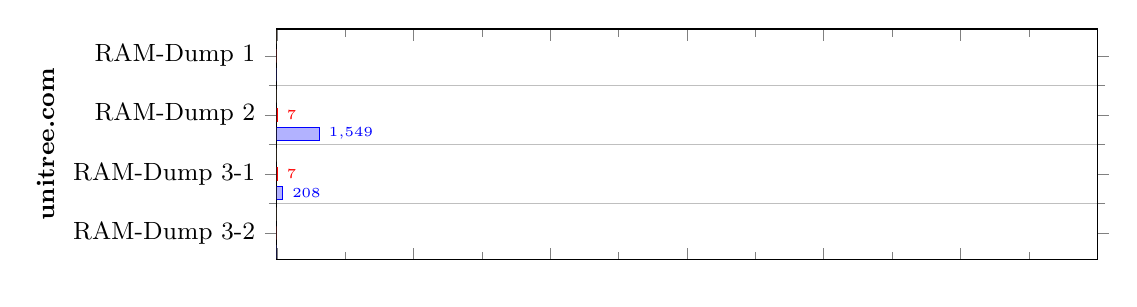
\begin{tikzpicture}
			\begin{axis}[
			xbar,
			width=12cm, 
			height=3cm, 
			ylabel style={align=center}, ylabel=\textbf{unitree.com},
			y=0.75cm,
			symbolic y coords={RAM-Dump 3-2, RAM-Dump 3-1, RAM-Dump 2, RAM-Dump 1},
			label style={font=\small},
			tick label style={font=\small},
			ytick=data,
			xticklabels={,,},
            xmin = 0,
            xmax = 30000,
			nodes near coords, 
			nodes near coords align={horizontal},
			nodes near coords style={font=\tiny},
   			nodes near coords={\pgfmathfloatifflags{\pgfplotspointmeta}{0}{}{\pgfmathprintnumber{\pgfplotspointmeta}}},
			bar width=.17cm,
			enlarge y limits={abs=2*\pgfplotbarwidth},
			scaled x ticks=false,
			legend style={
				at={(0.5,-0.1)},
				anchor=north
			},
			legend columns=3,
    		yminorgrids = true,minor tick num=1
			]
				\addplot coordinates {
				(0,RAM-Dump 3-2)  (208,RAM-Dump 3-1) (1549,RAM-Dump 2) (0,RAM-Dump 1)
				};
				\addplot coordinates {
				(0,RAM-Dump 3-2)  (7,RAM-Dump 3-1) (7,RAM-Dump 2) (0,RAM-Dump 1)
				};
				\addplot coordinates {
				(0,RAM-Dump 3-2)  (0,RAM-Dump 3-1) (0,RAM-Dump 2) (0,RAM-Dump 1)
				};
%				\legend{firefox.exe, tor.exe, Andere Prozesse}
			\end{axis}
		\end{tikzpicture}
		\\[-7pt]
		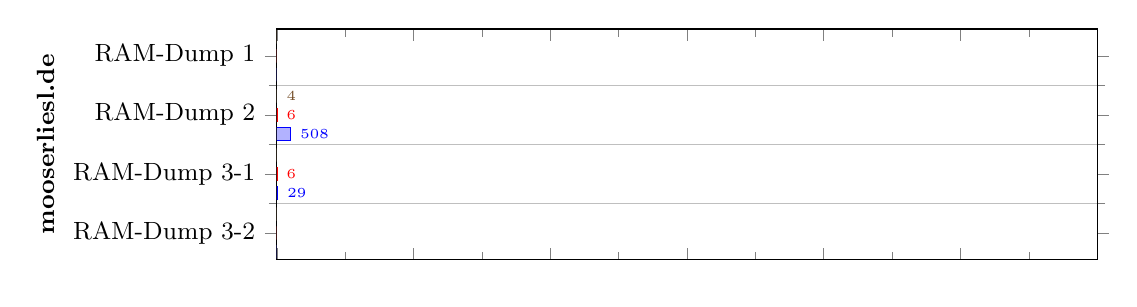
\begin{tikzpicture}
			\begin{axis}[
			xbar,
			width=12cm, 
			height=3cm, 
			ylabel style={align=center}, ylabel=\textbf{mooserliesl.de},
			y=0.75cm,
			symbolic y coords={RAM-Dump 3-2, RAM-Dump 3-1, RAM-Dump 2, RAM-Dump 1},
			label style={font=\small},
			tick label style={font=\small},
			ytick=data,
			xticklabels={,,},
            xmin = 0,
            xmax = 30000,
			nodes near coords, 
			nodes near coords align={horizontal},
			nodes near coords style={font=\tiny},
   			nodes near coords={\pgfmathfloatifflags{\pgfplotspointmeta}{0}{}{\pgfmathprintnumber{\pgfplotspointmeta}}},
			bar width=.17cm,
			enlarge y limits={abs=2*\pgfplotbarwidth},
			scaled x ticks=false,
			legend style={
				at={(0.5,-0.1)},
				anchor=north
			},
			legend columns=3,
    		yminorgrids = true,minor tick num=1
			]
				\addplot coordinates {
				(0,RAM-Dump 3-2)  (29,RAM-Dump 3-1) (508,RAM-Dump 2) (0,RAM-Dump 1)
				};
				\addplot coordinates {
				(0,RAM-Dump 3-2)  (6,RAM-Dump 3-1) (6,RAM-Dump 2) (0,RAM-Dump 1)
				};
				\addplot coordinates {
				(0,RAM-Dump 3-2)  (0,RAM-Dump 3-1) (4,RAM-Dump 2) (0,RAM-Dump 1)
				};
%				\legend{firefox.exe, tor.exe, Andere Prozesse}
			\end{axis}
		\end{tikzpicture}
		\\[-7pt]
		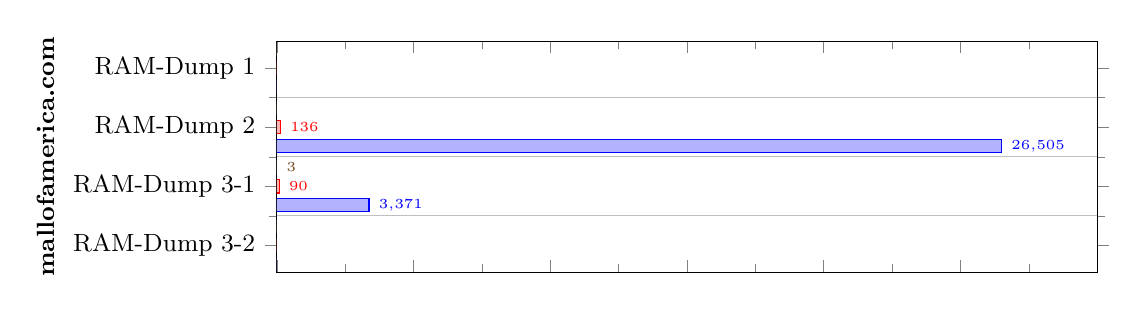
\begin{tikzpicture}
			\begin{axis}[
			xbar,
			width=12cm, 
			height=3cm, 
			ylabel style={align=center}, ylabel=\textbf{mallofamerica.com},
			y=0.75cm,
			symbolic y coords={RAM-Dump 3-2, RAM-Dump 3-1, RAM-Dump 2, RAM-Dump 1},
			label style={font=\small},
			tick label style={font=\small},
			ytick=data,
			xticklabels={,,},
            xmin = 0,
            xmax = 30000,
			nodes near coords, 
			nodes near coords align={horizontal},
			nodes near coords style={font=\tiny},
   			nodes near coords={\pgfmathfloatifflags{\pgfplotspointmeta}{0}{}{\pgfmathprintnumber{\pgfplotspointmeta}}},
			bar width=.17cm,
			enlarge y limits={abs=2*\pgfplotbarwidth},
			scaled x ticks=false,
			legend style={
				at={(0.5,-0.1)},
				anchor=north
			},
			legend columns=3,
    		yminorgrids = true,minor tick num=1
			]
				\addplot coordinates {
				(0,RAM-Dump 3-2)  (3371,RAM-Dump 3-1) (26505,RAM-Dump 2) (0,RAM-Dump 1)
				};
				\addplot coordinates {
				(0,RAM-Dump 3-2)  (90,RAM-Dump 3-1) (136,RAM-Dump 2) (0,RAM-Dump 1)
				};
				\addplot coordinates {
				(0,RAM-Dump 3-2)  (3,RAM-Dump 3-1) (0,RAM-Dump 2) (0,RAM-Dump 1)
				};
%				\legend{firefox.exe, tor.exe, Andere Prozesse}
			\end{axis}
		\end{tikzpicture}
		\\[-7pt]
		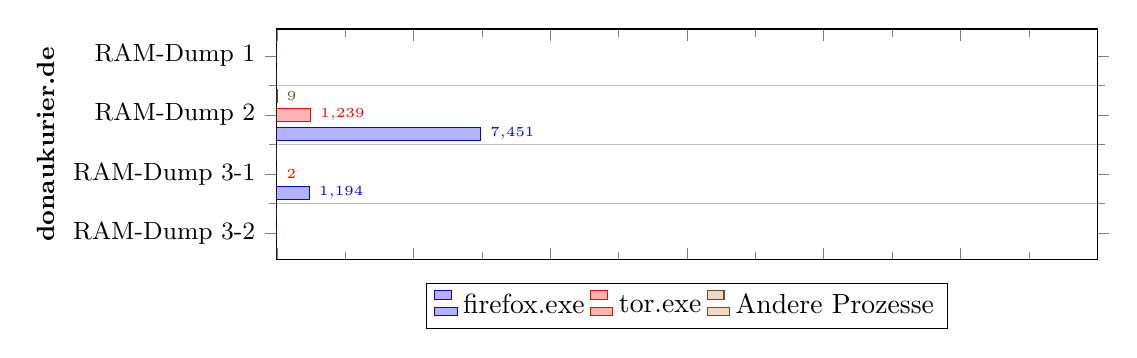
\begin{tikzpicture}
			\begin{axis}[
			xbar,
			width=12cm, 
			height=3cm, 
			ylabel style={align=center}, ylabel=\textbf{donaukurier.de},
			y=0.75cm,
			symbolic y coords={RAM-Dump 3-2, RAM-Dump 3-1, RAM-Dump 2, RAM-Dump 1},
			label style={font=\small},
			tick label style={font=\small},
			ytick=data,
			xticklabels={,,},
            xmin = 0,
            xmax = 30000,
			nodes near coords, 
			nodes near coords align={horizontal},
			nodes near coords style={font=\tiny},
   			nodes near coords={\pgfmathfloatifflags{\pgfplotspointmeta}{0}{}{\pgfmathprintnumber{\pgfplotspointmeta}}},
			bar width=.17cm,
			enlarge y limits={abs=2*\pgfplotbarwidth},
			scaled x ticks=false,
			legend style={
				at={(0.5,-0.1)},
				anchor=north
			},
			legend columns=3,
    		yminorgrids = true,minor tick num=1
			]
				\addplot coordinates {
				(0,RAM-Dump 3-2)  (1194,RAM-Dump 3-1) (7451,RAM-Dump 2) (0,RAM-Dump 1)
				};
				\addplot coordinates {
				(0,RAM-Dump 3-2)  (2,RAM-Dump 3-1) (1239,RAM-Dump 2) (0,RAM-Dump 1)
				};
				\addplot coordinates {
				(0,RAM-Dump 3-2)  (0,RAM-Dump 3-1) (9,RAM-Dump 2) (0,RAM-Dump 1)
				};
				\legend{firefox.exe, tor.exe, Andere Prozesse}
			\end{axis}
		\end{tikzpicture}
	\end{tabular}
	}
	\captionof{figure}{Tor-Browser: Anzahl gefundener URL-Artefakte im RAM}
	\label{chart:tor-volatility-urls}
\end{table}
%\begin{figure}[h!]
%	\centerline{\resizebox{\linewidth}{!}{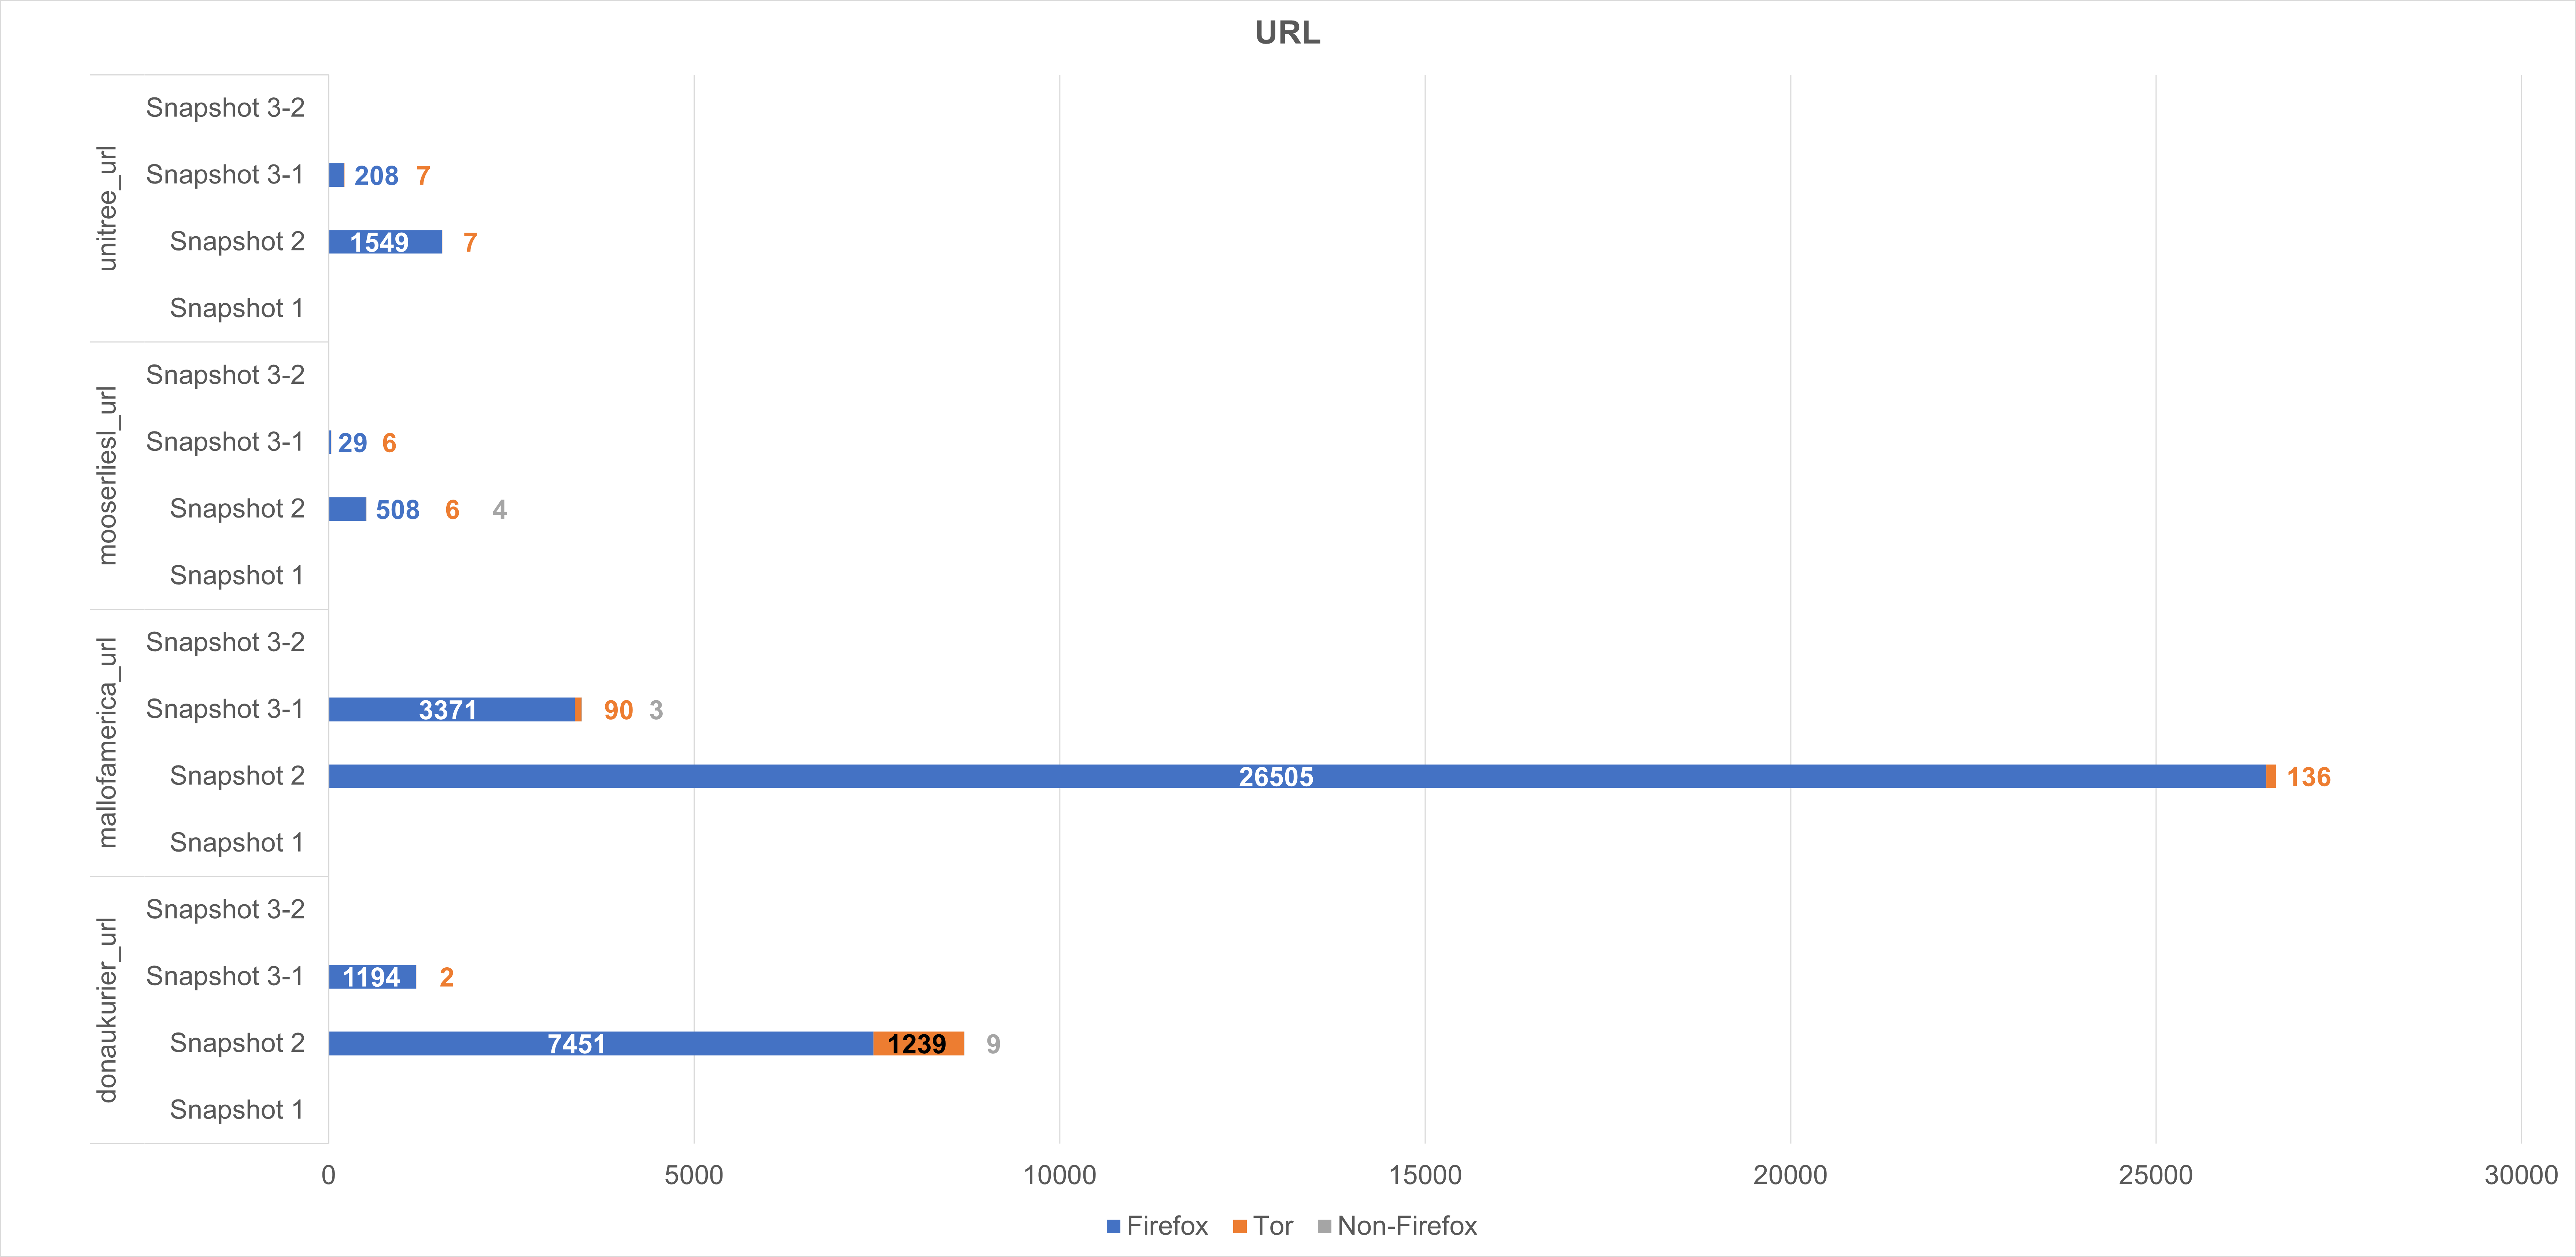
\includegraphics{bilder/volatility/tor/url.png}}}
%	\label{chart:final-criteria}  
%	\caption{URL}
%\end{figure}


\begin{table}[h!]
	\resizebox{\linewidth}{!}{
	\begin{tabular}{r}	
		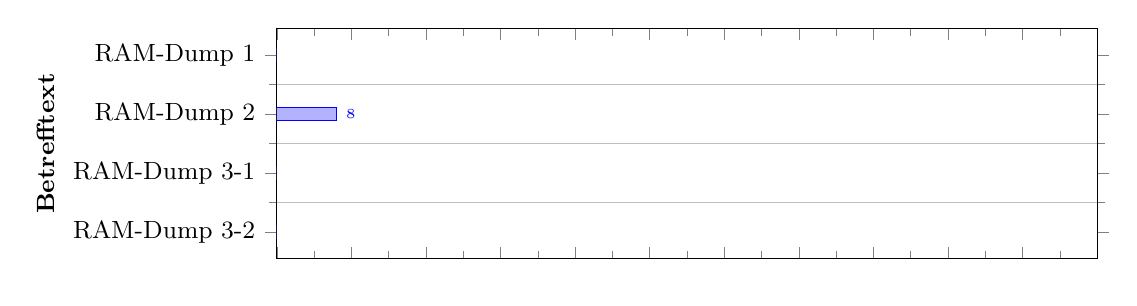
\begin{tikzpicture}					
			\begin{axis}[
			xbar,
			width=12cm, 
			height=3cm, 
			ylabel style={align=center}, ylabel=\textbf{Betrefftext},
			y=0.75cm,
			symbolic y coords={RAM-Dump 3-2, RAM-Dump 3-1, RAM-Dump 2, RAM-Dump 1},
			label style={font=\small},
			tick label style={font=\small},
			ytick=data,
			xticklabels={,,},
            xmin = 0,
            xmax = 110,
			nodes near coords, 
			nodes near coords align={horizontal},
			nodes near coords style={font=\tiny},
   			nodes near coords={\pgfmathfloatifflags{\pgfplotspointmeta}{0}{}{\pgfmathprintnumber{\pgfplotspointmeta}}},
			bar width=.17cm,
			enlarge y limits={abs=2*\pgfplotbarwidth},
			scaled x ticks=false,
			legend style={
				at={(0.5,-0.1)},
				anchor=north
			},
			legend columns=3,
    		yminorgrids = true,minor tick num=1
			]
				\addplot coordinates {
				(0,RAM-Dump 3-2)  (0,RAM-Dump 3-1) (8,RAM-Dump 2) (0,RAM-Dump 1)
				};
%				\addplot coordinates {
%				(0,RAM-Dump 3-2)  (0,RAM-Dump 3-1) (0,RAM-Dump 2) (0,RAM-Dump 1)
%				};
%				\addplot coordinates {
%				(0,RAM-Dump 3-2)  (0,RAM-Dump 3-1) (0,RAM-Dump 2) (0,RAM-Dump 1)
%				};
%				\legend{firefox.exe, tor.exe, Andere Prozesse}
			\end{axis}
		\end{tikzpicture}
		\\[-7pt]
		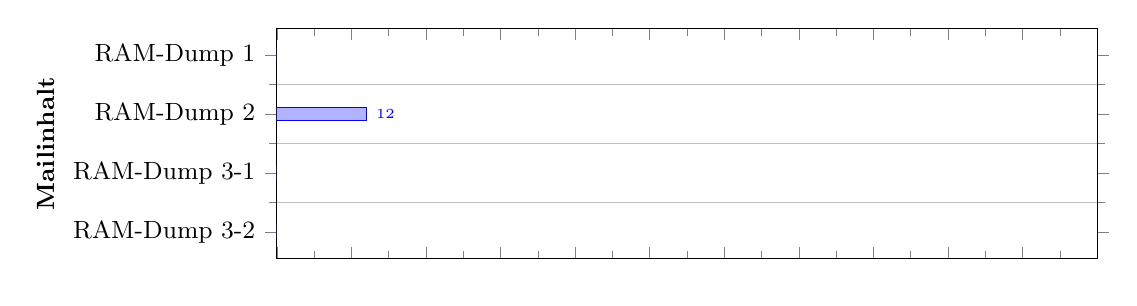
\begin{tikzpicture}
			\begin{axis}[
			xbar,
			width=12cm, 
			height=3cm, 
			ylabel style={align=center}, ylabel=\textbf{Mailinhalt},
			y=0.75cm,
			symbolic y coords={RAM-Dump 3-2, RAM-Dump 3-1, RAM-Dump 2, RAM-Dump 1},
			label style={font=\small},
			tick label style={font=\small},
			ytick=data,
			xticklabels={,,},
            xmin = 0,
            xmax = 110,
			nodes near coords, 
			nodes near coords align={horizontal},
			nodes near coords style={font=\tiny},
   			nodes near coords={\pgfmathfloatifflags{\pgfplotspointmeta}{0}{}{\pgfmathprintnumber{\pgfplotspointmeta}}},
			bar width=.17cm,
			enlarge y limits={abs=2*\pgfplotbarwidth},
			scaled x ticks=false,
			legend style={
				at={(0.5,-0.1)},
				anchor=north
			},
			legend columns=3,
    		yminorgrids = true,minor tick num=1
			]
				\addplot coordinates {
				(0,RAM-Dump 3-2)  (0,RAM-Dump 3-1) (12,RAM-Dump 2) (0,RAM-Dump 1)
				};
%				\addplot coordinates {
%				(0,RAM-Dump 3-2)  (0,RAM-Dump 3-1) (0,RAM-Dump 2) (0,RAM-Dump 1)
%				};
%				\addplot coordinates {
%				(0,RAM-Dump 3-2)  (0,RAM-Dump 3-1) (0,RAM-Dump 2) (0,RAM-Dump 1)
%				};
%				\legend{firefox.exe, tor.exe, Andere Prozesse}
			\end{axis}
		\end{tikzpicture}
		\\[-7pt]
		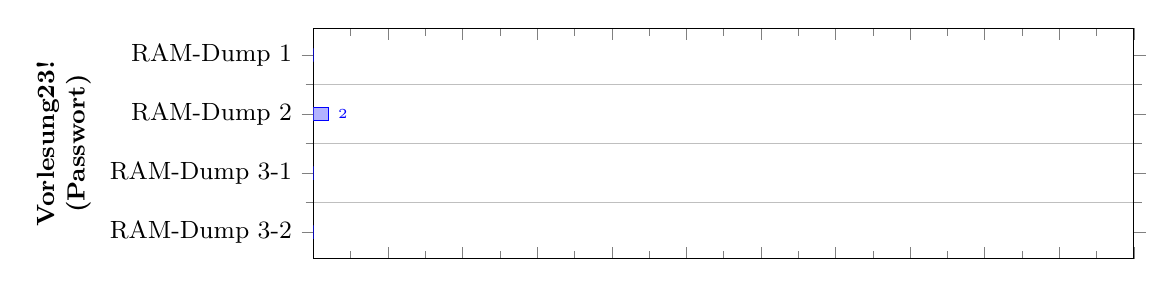
\begin{tikzpicture}
			\begin{axis}[
			xbar,
			width=12cm, 
			height=3cm, 
			ylabel style={align=center}, ylabel=\textbf{Vorlesung23!}\\\textbf{(Passwort)},
			y=0.75cm,
			symbolic y coords={RAM-Dump 3-2, RAM-Dump 3-1, RAM-Dump 2, RAM-Dump 1},
			label style={font=\small},
			tick label style={font=\small},
			ytick=data,
			xticklabels={,,},
            xmin = 0,
            xmax = 110,
			nodes near coords, 
			nodes near coords align={horizontal},
			nodes near coords style={font=\tiny},
   			nodes near coords={\pgfmathfloatifflags{\pgfplotspointmeta}{0}{}{\pgfmathprintnumber{\pgfplotspointmeta}}},
			bar width=.17cm,
			enlarge y limits={abs=2*\pgfplotbarwidth},
			scaled x ticks=false,
			legend style={
				at={(0.5,-0.1)},
				anchor=north
			},
			legend columns=3,
    		yminorgrids = true,minor tick num=1
			]
				\addplot coordinates {
				(0,RAM-Dump 3-2)  (0,RAM-Dump 3-1) (2,RAM-Dump 2) (0,RAM-Dump 1)
				};
%				\addplot coordinates {
%				(0,RAM-Dump 3-2)  (0,RAM-Dump 3-1) (0,RAM-Dump 2) (0,RAM-Dump 1)
%				};
%				\addplot coordinates {
%				(0,RAM-Dump 3-2)  (0,RAM-Dump 3-1) (0,RAM-Dump 2) (0,RAM-Dump 1)
%				};
%				\legend{firefox.exe, tor.exe, Andere Prozesse}
			\end{axis}
		\end{tikzpicture}
		\\[-8pt]
		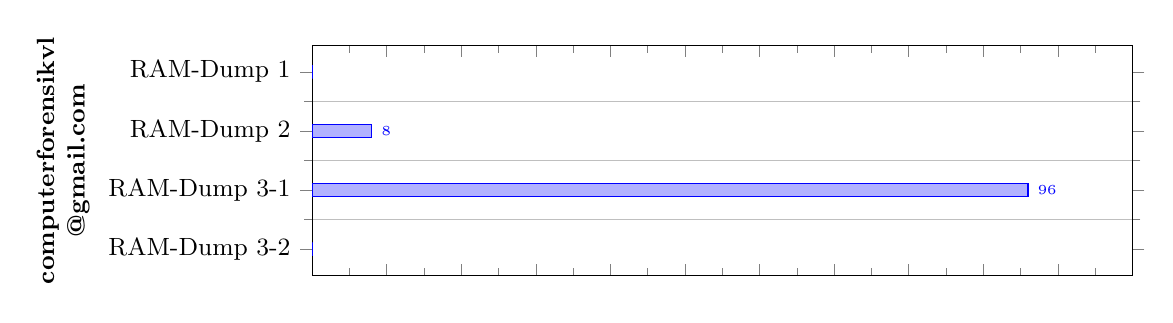
\begin{tikzpicture}
			\begin{axis}[
			xbar,
			width=12cm, 
			height=3cm, 
			ylabel style={align=center}, ylabel=\textbf{computerforensikvl}\\\textbf{@gmail.com},
			y=0.75cm,
			symbolic y coords={RAM-Dump 3-2, RAM-Dump 3-1, RAM-Dump 2, RAM-Dump 1},
			label style={font=\small},
			tick label style={font=\small},
			ytick=data,
			xticklabels={,,},
            xmin = 0,
            xmax = 110,
			nodes near coords, 
			nodes near coords align={horizontal},
			nodes near coords style={font=\tiny},
   			nodes near coords={\pgfmathfloatifflags{\pgfplotspointmeta}{0}{}{\pgfmathprintnumber{\pgfplotspointmeta}}},
			bar width=.17cm,
			enlarge y limits={abs=2*\pgfplotbarwidth},
			scaled x ticks=false,
			legend style={
				at={(0.5,-0.1)},
				anchor=north
			},
			legend columns=3,
    		yminorgrids = true,minor tick num=1
			]
				\addplot coordinates {
				(0,RAM-Dump 3-2)  (96,RAM-Dump 3-1) (8,RAM-Dump 2) (0,RAM-Dump 1)
				};
%				\addplot coordinates {
%				(0,RAM-Dump 3-2)  (0,RAM-Dump 3-1) (0,RAM-Dump 2) (0,RAM-Dump 1)
%				};
%				\addplot coordinates {
%				(0,RAM-Dump 3-2)  (0,RAM-Dump 3-1) (0,RAM-Dump 2) (0,RAM-Dump 1)
%				};
%				\legend{firefox.exe, tor.exe, Andere Prozesse}
			\end{axis}
		\end{tikzpicture}
		\\[-7pt]
		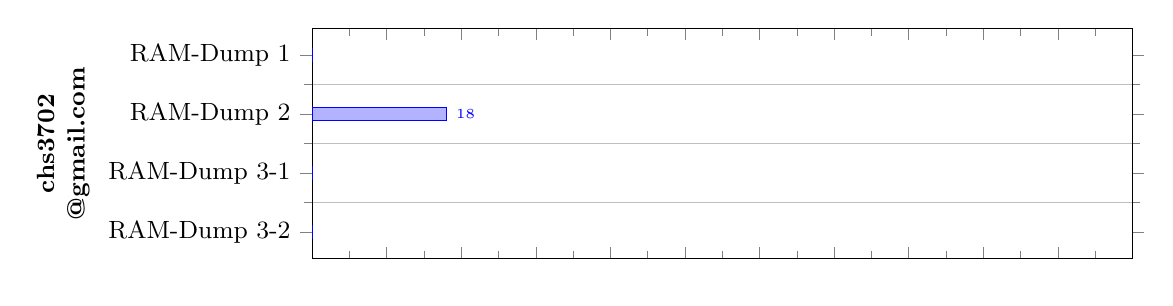
\begin{tikzpicture}
			\begin{axis}[
			xbar,
			width=12cm, 
			height=3cm, 
			ylabel style={align=center}, ylabel=\textbf{chs3702}\\\textbf{@gmail.com},
			y=0.75cm,
			symbolic y coords={RAM-Dump 3-2, RAM-Dump 3-1, RAM-Dump 2, RAM-Dump 1},
			label style={font=\small},
			tick label style={font=\small},
			ytick=data,
			xticklabels={,,},
            xmin = 0,
            xmax = 110,
			nodes near coords, 
			nodes near coords align={horizontal},
			nodes near coords style={font=\tiny},
   			nodes near coords={\pgfmathfloatifflags{\pgfplotspointmeta}{0}{}{\pgfmathprintnumber{\pgfplotspointmeta}}},
			bar width=.17cm,
			enlarge y limits={abs=2*\pgfplotbarwidth},
			scaled x ticks=false,
			legend style={
				at={(0.5,-0.1)},
				anchor=north
			},
			legend columns=3,
    		yminorgrids = true,minor tick num=1
			]
				\addplot coordinates {
				(0,RAM-Dump 3-2)  (0,RAM-Dump 3-1) (18,RAM-Dump 2) (0,RAM-Dump 1)
				};
%				\addplot coordinates {
%				(0,RAM-Dump 3-2)  (0,RAM-Dump 3-1) (0,RAM-Dump 2) (0,RAM-Dump 1)
%				};
%				\addplot coordinates {
%				(0,RAM-Dump 3-2)  (0,RAM-Dump 3-1) (0,RAM-Dump 2) (0,RAM-Dump 1)
%				};
%				\legend{firefox.exe, tor.exe, Andere Prozesse}
			\end{axis}
		\end{tikzpicture}
		\\[-7pt]
		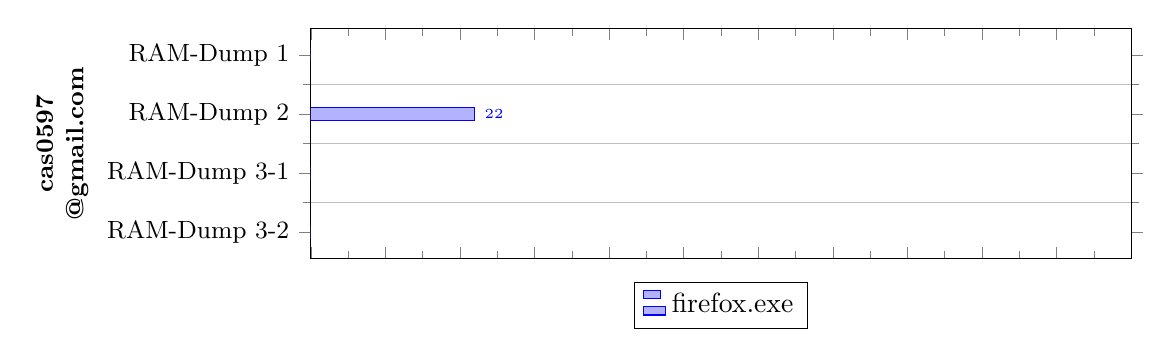
\begin{tikzpicture}
			\begin{axis}[
			xbar,
			width=12cm, 
			height=3cm, 
			ylabel style={align=center}, ylabel=\textbf{cas0597}\\\textbf{@gmail.com},
			y=0.75cm,
			symbolic y coords={RAM-Dump 3-2, RAM-Dump 3-1, RAM-Dump 2, RAM-Dump 1},
			label style={font=\small},
			tick label style={font=\small},
			ytick=data,
			xticklabels={,,},
            xmin = 0,
            xmax = 110,
			nodes near coords, 
			nodes near coords align={horizontal},
			nodes near coords style={font=\tiny},
   			nodes near coords={\pgfmathfloatifflags{\pgfplotspointmeta}{0}{}{\pgfmathprintnumber{\pgfplotspointmeta}}},
			bar width=.17cm,
			enlarge y limits={abs=2*\pgfplotbarwidth},
			scaled x ticks=false,
			legend style={
				at={(0.5,-0.1)},
				anchor=north
			},
			legend columns=3,
    		yminorgrids = true,minor tick num=1
			]
				\addplot coordinates {
				(0,RAM-Dump 3-2)  (0,RAM-Dump 3-1) (22,RAM-Dump 2) (0,RAM-Dump 1)
				};
%				\addplot coordinates {
%				(0,RAM-Dump 3-2)  (0,RAM-Dump 3-1) (0,RAM-Dump 2) (0,RAM-Dump 1)
%				};
%				\addplot coordinates {
%				(0,RAM-Dump 3-2)  (0,RAM-Dump 3-1) (0,RAM-Dump 2) (0,RAM-Dump 1)
%				};
				\legend{firefox.exe}
			\end{axis}
		\end{tikzpicture}
	\end{tabular}
	}
	\captionof{figure}{Tor-Browser: Anzahl gefundener E-Mail Artefakte im RAM}
	\label{chart:tor-volatility-mail}
\end{table}
%\begin{figure}[h!]
%	\centerline{\resizebox{\linewidth}{!}{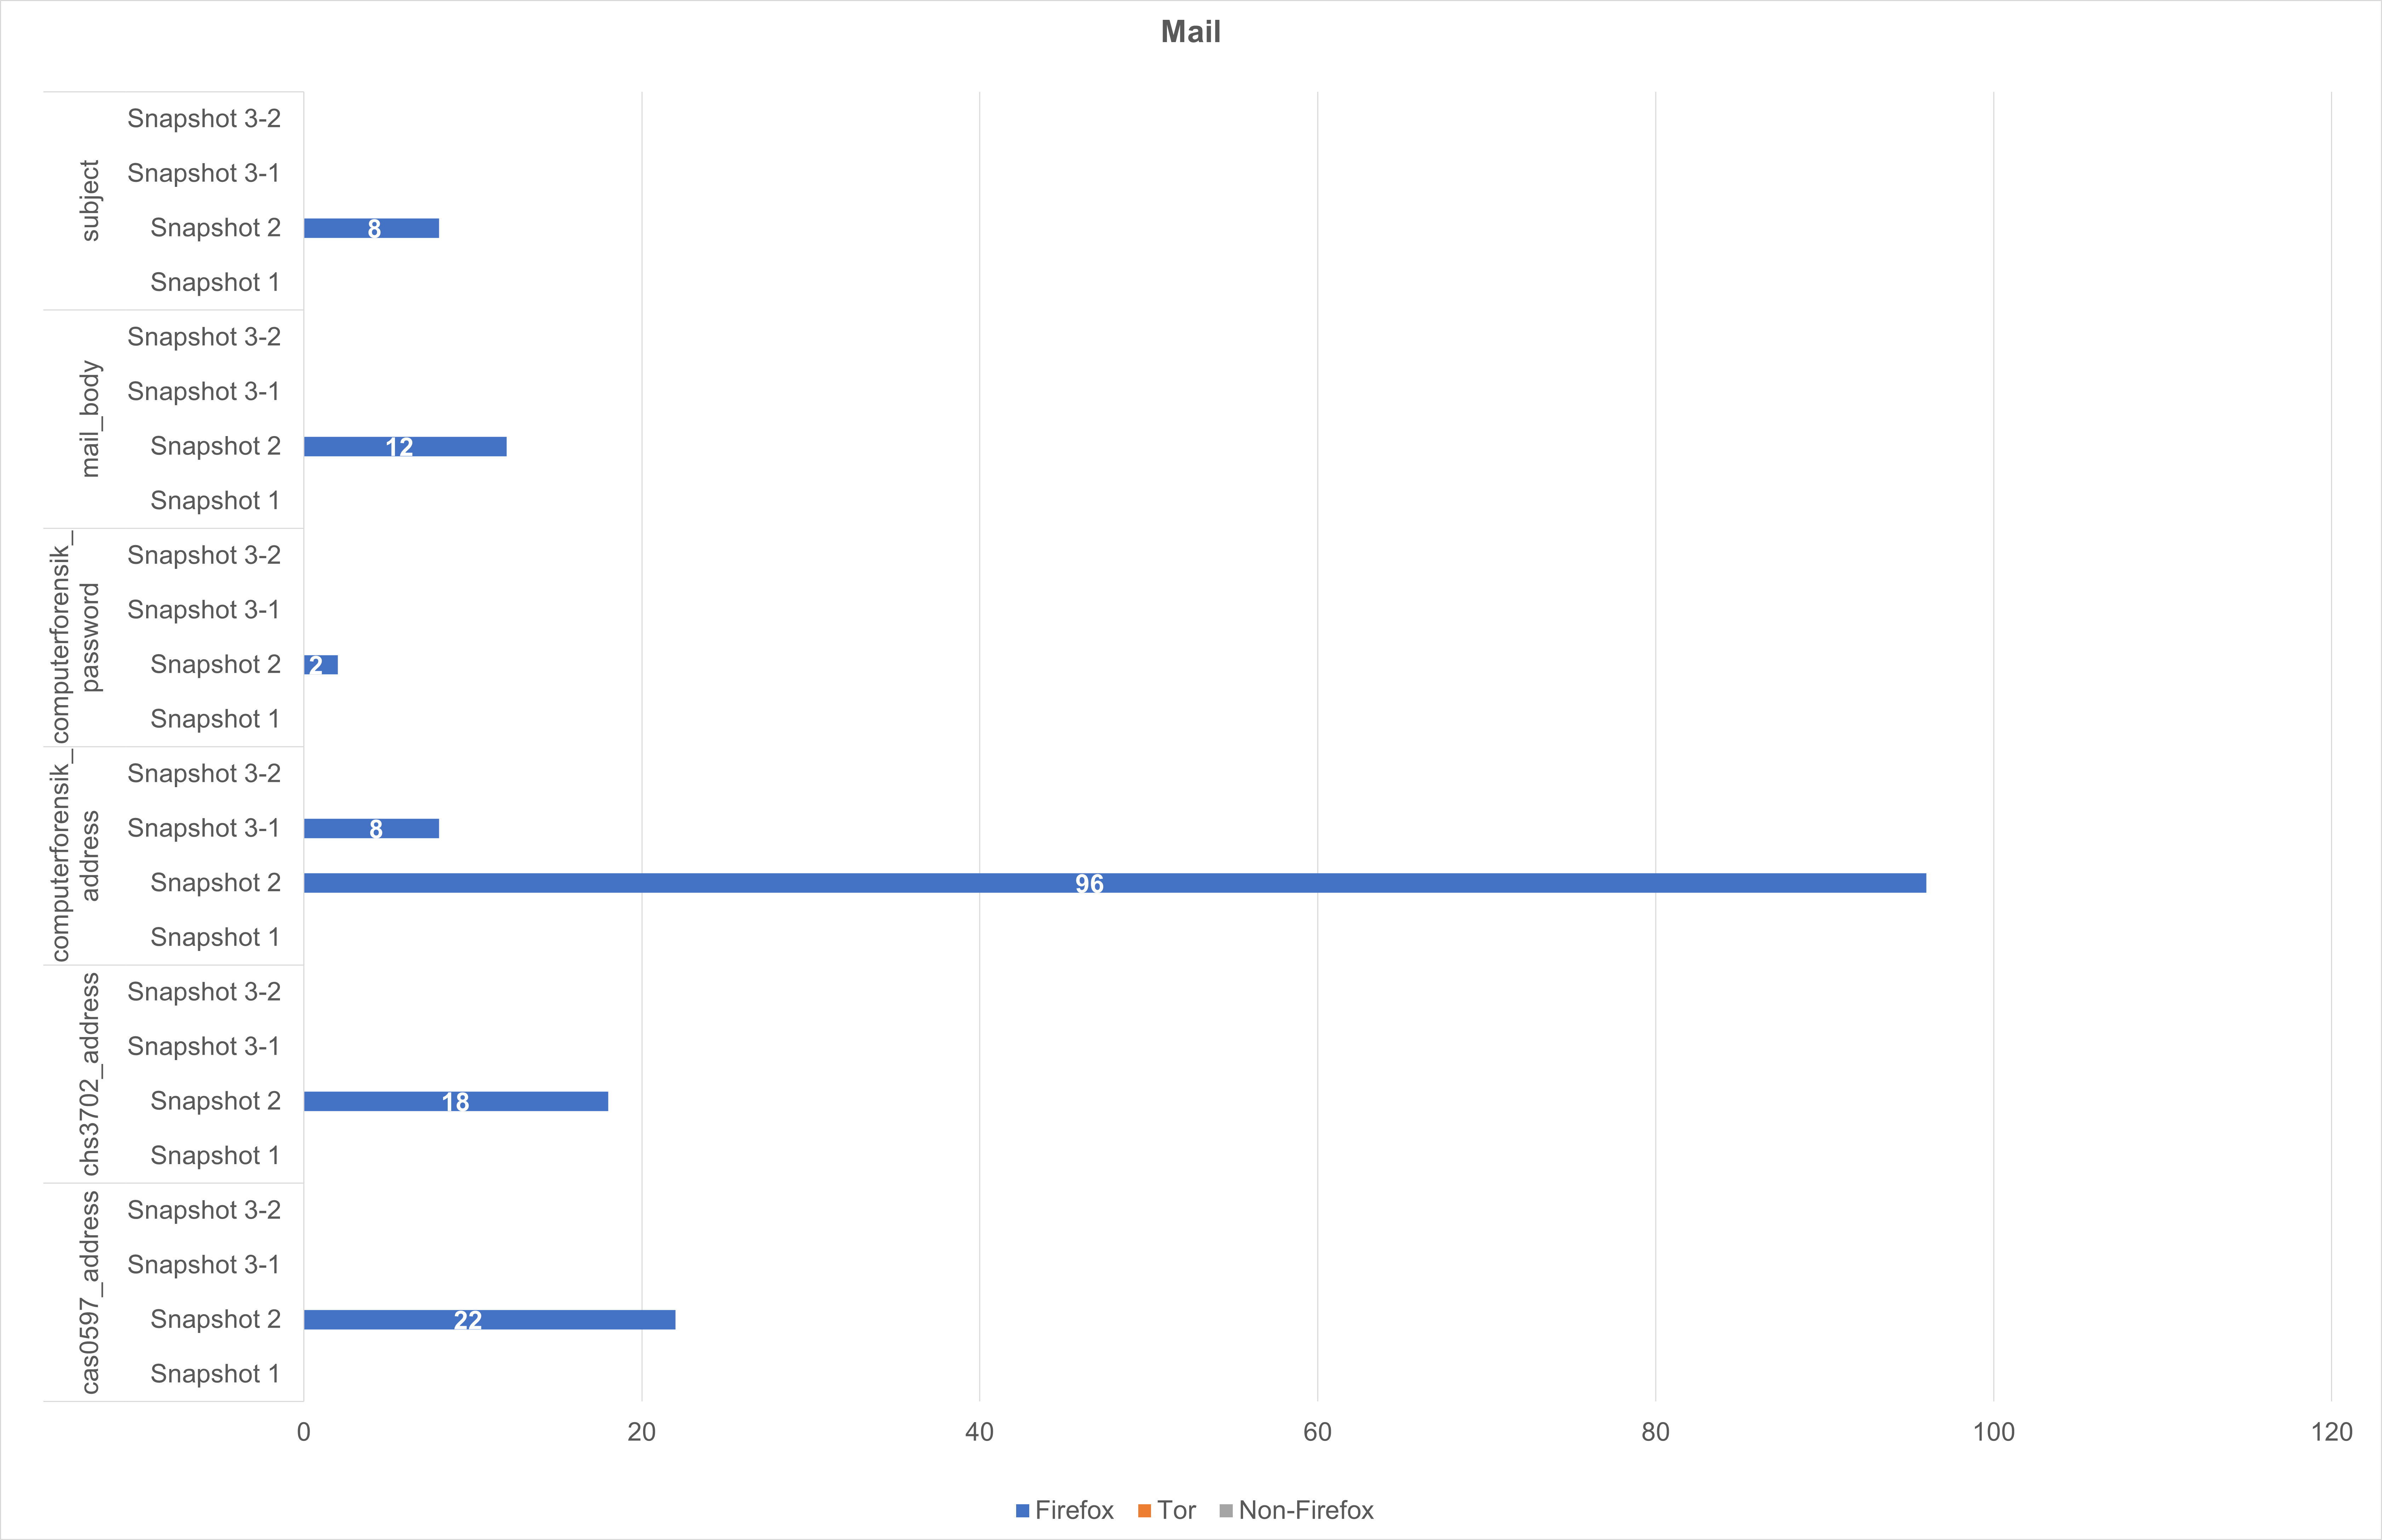
\includegraphics{bilder/volatility/tor/mail.png}}}
%	\label{chart:final-criteria}  
%	\caption{Mail}
%\end{figure}
\paragraph*{Yara-Regel \glqq{}E-Mail\grqq{}}
Nach dem Browsing-Szenario, vor Zuweisung einer \glqq{}Neuen Identität\grqq{} (RAM-Dump 2), konnten alle Kategorien von E-Mail-Artefakten gefunden werden.
Nur die Absenderadresse \glqq{}computerforensikvl@gmail.com\grqq{} wurde noch nach Erstellen der \glqq{}Neuen Identität\grqq{} (RAM-Dump 3-1) gefunden. Die Absenderadresse ist ebenso das am häufigsten gefundene E-Mail Artefakt.
Wie in Abbildung \ref{chart:tor-volatility-mail} dargestellt, wurden die Artefakte ausschließlich in Firefox-Prozessen gefunden.
Wie bei der Analyse der Firefox RAM-Dumps in Abschnitt \ref{subsubsection:ergebnisse-firefox-uncommonlocations-analysemitvolatility}, wurde das Passwort als Klartext nach dem Browsing-Szenario, vor Zuweisung einer \glqq{}Neuen Identität\grqq{}(RAM-Dump 2) gefunden.

\begin{table}[h!]
	\centering
	\caption{Tor-Browser: Abbildung der virtuellen Speicheradressen der gefundenen Strings im RAM auf Byte-Offsets der entsprechenden Speicherseiten}
	\label{tab:tor-mapping-virtaddr-to-byteoffset}
	\resizebox{\linewidth}{!}{
	\begin{tabular}{|c|c|c|ll}
	\cline{1-3}
	\textbf{Virtuelle Speicheradresse} & \textbf{PID} & \textbf{Byte-Offset in extrahierter Speicherseite} &  &  \\ \cline{1-3}
	0x2b1e2c22318                      & 708         & 0xea0318                                         &  &  \\ \cline{1-3}
	0x2b1e2ecb748                     & 708         & 0x10f7748                                         &  &  \\ \cline{1-3}
	\end{tabular}
	}
\end{table}

Das Passwort wurde zweimal im Firefox Prozess mit der PID 708 gefunden. Tabelle \ref{tab:tor-mapping-virtaddr-to-byteoffset} zeigt die virtuellen Speicheradressen der Artefakte aus der Yarascan Ausgabe sowie deren Abbildung auf die mithilfe des Volatility Plugins \textit{memmap} identifizierten Byte-Offsets der extrahierten Speicherseiten.


\begin{figure}[h!]
	\centering
	\subcaptionbox{Byte-Offset 0xea0318}{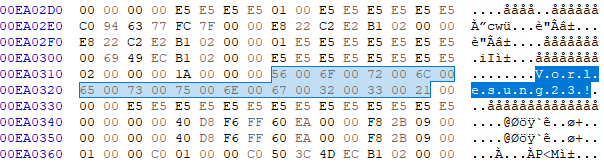
\includegraphics[width=0.47\textwidth]{bilder/volatility/tor/password_0xea0318.png}}%
	\hfill
	\subcaptionbox{Byte-Offset 0x10f7748}{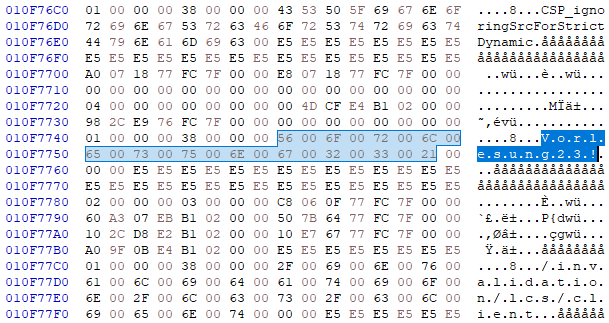
\includegraphics[width=0.47\textwidth]{bilder/volatility/tor/password_0x10f7748.png}}%
	\caption{Tor-Browser: Passwort-Klartext in Speicherseiten von PID 708}
	\label{img:firefox-pw-offset-pid-708}  
\end{figure}
Bei Untersuchung des String-Kontexts in Abbildung \ref{img:firefox-pw-offset-pid-708}, wurden für das Passwort am Byte-Offset 0xea0318 keine auffälligen Artefakte entdeckt.
Im Bereich des gefundenen Passworts am Byte-Offset 0x10f7748 befindet sich der String \glqq{}CSP\_ignoringSrcForStrictDynamic\grqq{}, dessen Bedeutung nicht näher bestimmt werden konnte.
Weiterhin wurde die Zeichenkette \glqq{}invalidation/lcs/client\grqq{} in der Nähe des Passworts gefunden. Auf diesen String wird in einem Firefox Bug-Ticket verwiesen, welches bereits 2017 geschlossen wurde. Der Bug betraf ein Speicher-Leck. \cite{Bugzilla.05.06.2023} Der genaue Zusammenhang mit dem gefundenen Passwort konnte nicht ermittelt werden. 
	
\paragraph*{Yara-Regel \glqq{}DK-Logo\grqq{}}
Wie in Abbildung \ref{chart:tor-volatility-image} dargestellt, wurde der Hexadezimal-Wert des Donaukurier-Logos ein einziges Mal nach dem Browsing-Szenario, vor Erstellen der \glqq{}Neuen Identität\grqq{} (RAM-Dump 2) in einem Firefox Prozess gefunden.
\begin{figure}[h!]
	\resizebox{\linewidth}{!}{
		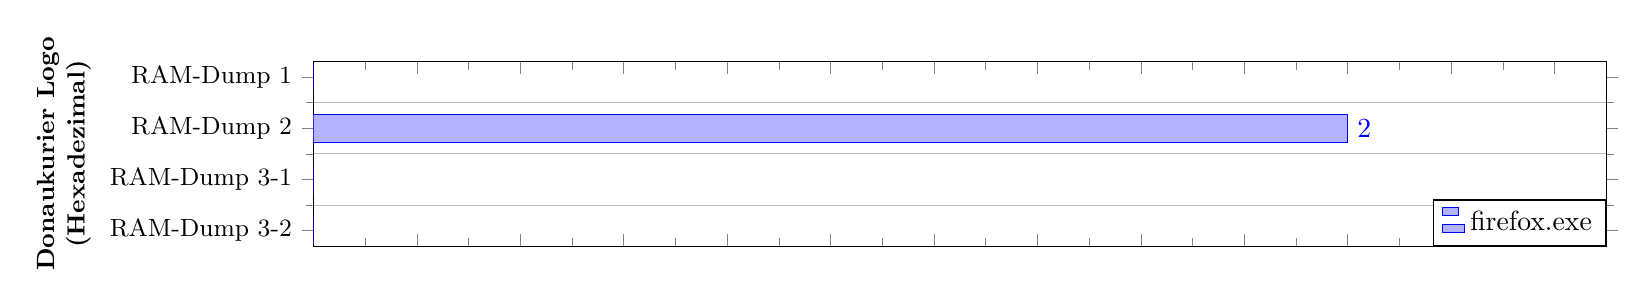
\begin{tikzpicture}
			\begin{axis}[
			xbar,
			width=18cm, 
			height=12cm, 
			ylabel style={align=center}, ylabel=\textbf{Donaukurier Logo}\\\textbf{(Hexadezimal)},
			y=0.65cm,
			symbolic y coords={RAM-Dump 3-2, RAM-Dump 3-1, RAM-Dump 2, RAM-Dump 1},
			label style={font=\small},
			tick label style={font=\small},
			ytick=data,
			xticklabels={,,},
            xmin = 0,
            xmax = 2.5,
			nodes near coords, 
			nodes near coords align={horizontal},
   			nodes near coords={\pgfmathfloatifflags{\pgfplotspointmeta}{0}{}{\pgfmathprintnumber{\pgfplotspointmeta}}},	
			legend style={
				at={(1,0)},
				anchor=south east
			},
			legend columns=2,
    		yminorgrids = true,minor tick num=1
			]
				\addplot coordinates {
				(0,RAM-Dump 3-2)  (0,RAM-Dump 3-1) (2,RAM-Dump 2) (0,RAM-Dump 1)
				};
				\legend{firefox.exe}
			\end{axis}
		\end{tikzpicture}
	}
	\caption{Tor-Browser: Anzahl gefundener Hexadezimalwerte des Donaukurier-Logos im RAM}
	\label{chart:tor-volatility-image}
\end{figure}
%\begin{figure}[h!]
%	\centerline{\resizebox{\linewidth}{!}{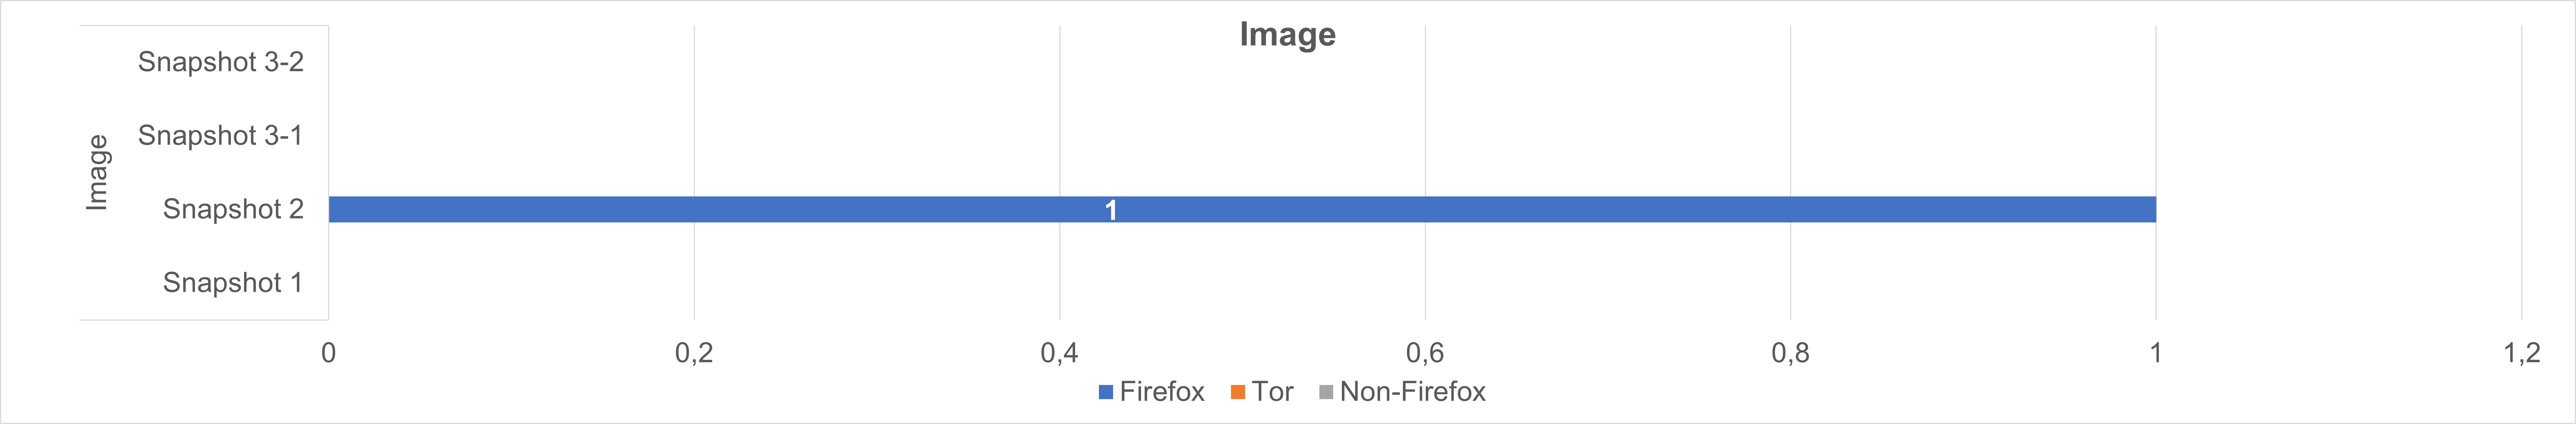
\includegraphics{bilder/volatility/tor/image.png}}}
%	\label{chart:final-criteria}  
%	\caption{Image}
%\end{figure}


%\begin{figure}[h!]
%	\centerline{\resizebox{\linewidth}{!}{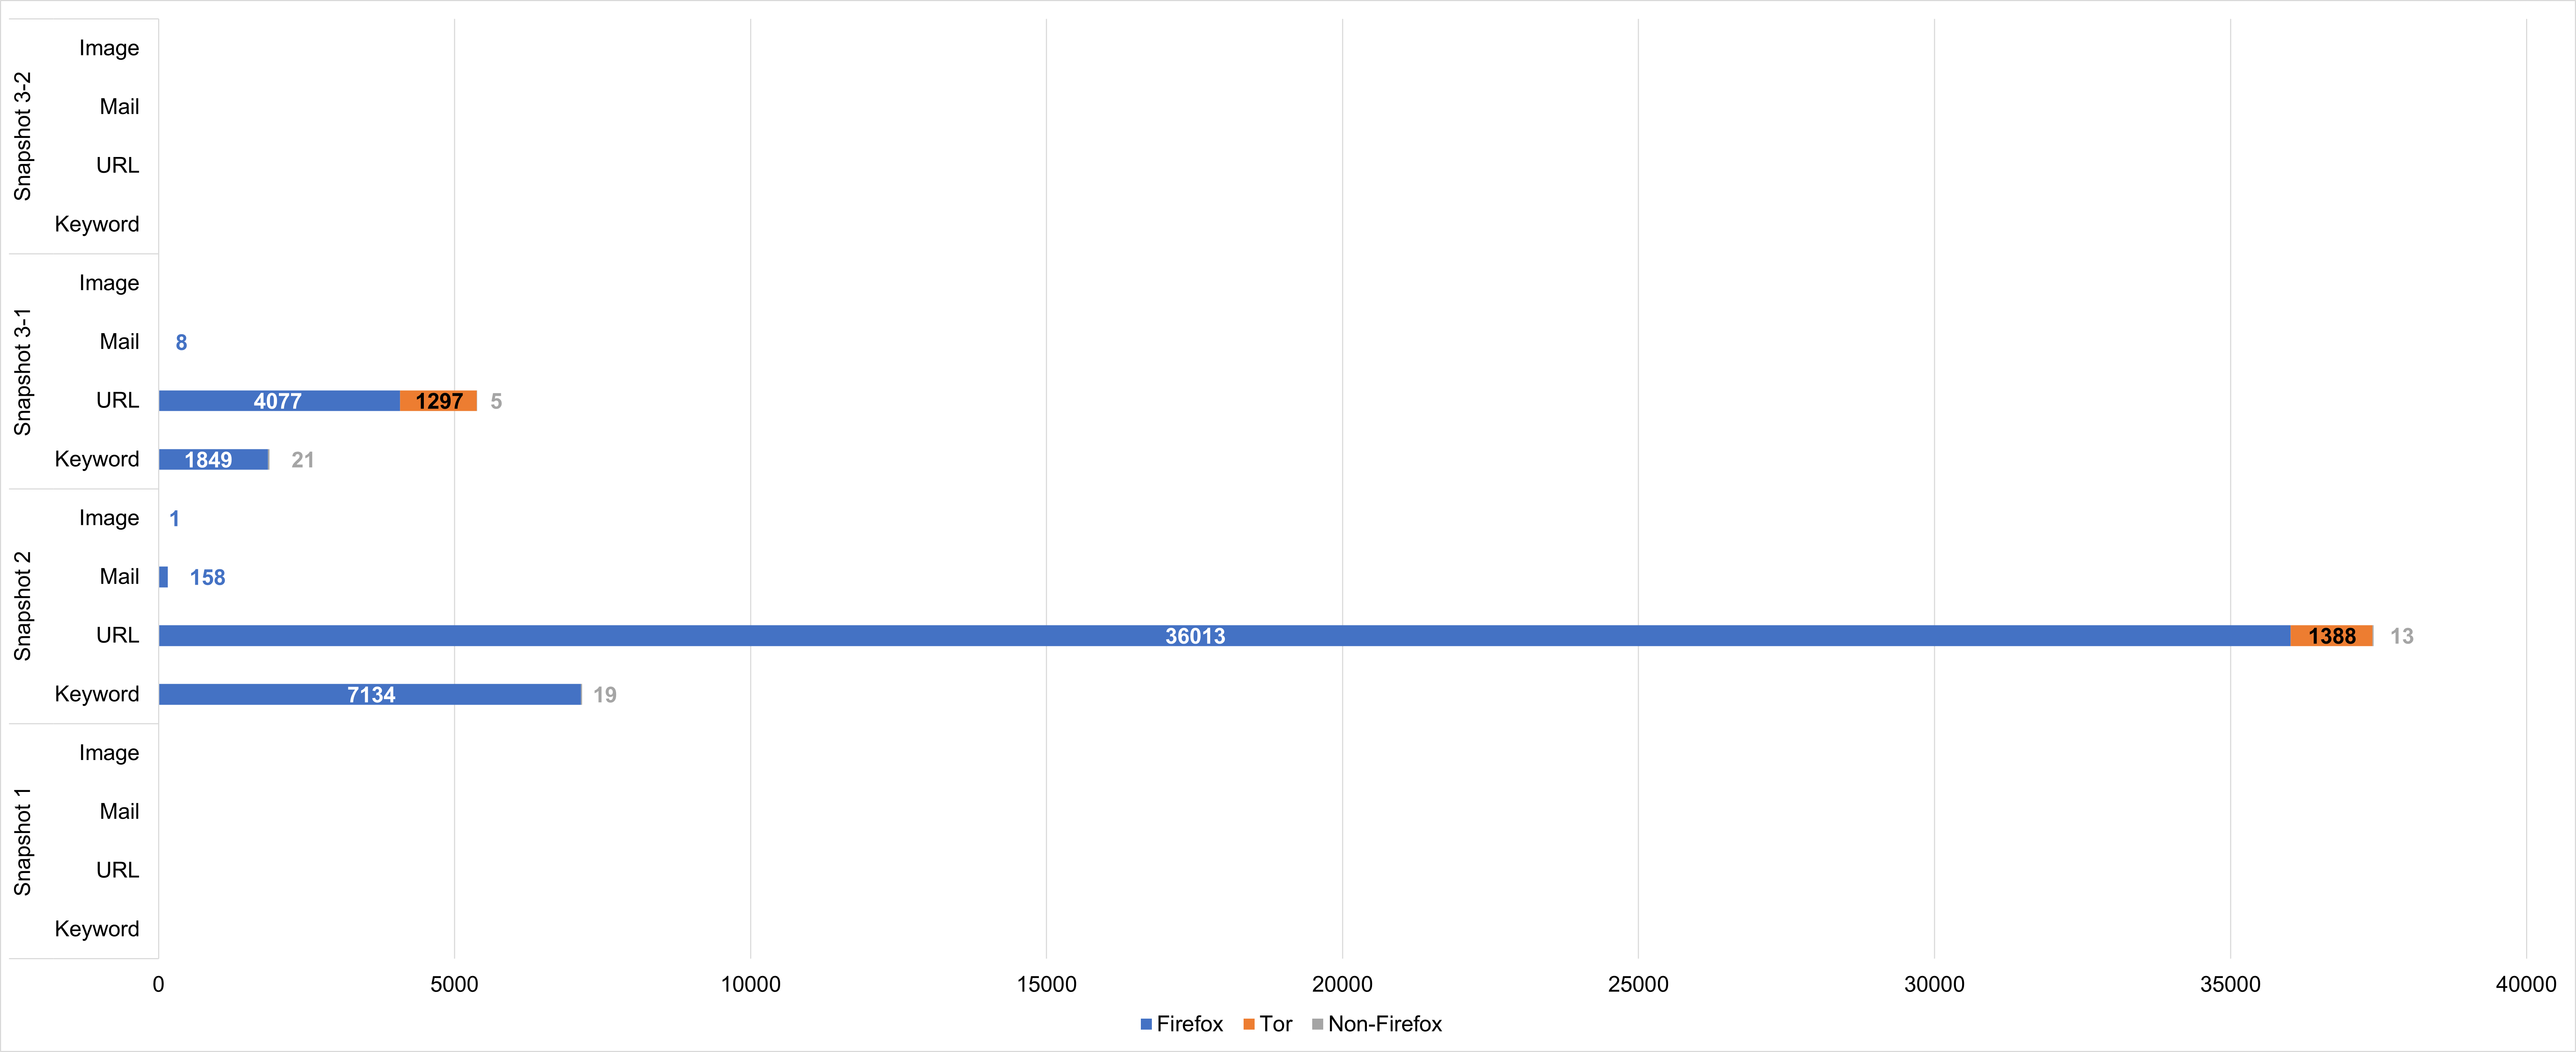
\includegraphics{bilder/volatility/tor/summary.png}}}
%	\label{chart:final-criteria}  
%	\caption{Summary}
%\end{figure}
%Literatur:
%o Autopsy: \cite{Muir.2019}
%	•	Configuration files, downloaded files, and browserrelated data are recoverable from the file system.
%	•	Significant data-leakage from the browsing session occurred: HTTP header information, titles of web pages and an instance of a URL were found in registry files, system files, and unallocated space.
%o RAM-Analyse nach \cite{Muir.2019}:
%	•	Live-Analyse identifiziert auch nach dem Schließen und Deinstallieren des Browsers und Abmelden des Benutzers Spuren von Tor-Prozessen, einschließlich des absoluten Pfads zur Browser-Executable, des Benutzernamens und des Geräts, von dem es ausgeführt wurde.
%	•	The data-leakage contained the German word for ’search’ in reference to a Google search. This hints at the locale of the Tor server used to exit the network (exit relay).
%
%o RAM-Analyse nach \cite{Hariharan.2022}:
%	o	process was found to be firefox.exe
%	o	pslist and pstree: parent process was shown 
%	o	Belkasoft Ram Capturer: retrieve information about facebook
%	o	Cmdline: file path of the browser “E:/TorBrowser/Browser/firefox.exe” + name of process tor.exe and firefox.exe
%	o	Dlllist: DLL files of the executable files were not captured
%	o	Netscan: tor.exe + obfs4proxy.exe -> showed “LISTENING” connections to nonstandardized ports as output.
%	Yarascan: was able to retrieve all the browsing sessions
%o RAM-Analyse nach \cite{Sajan.2021} mit Volatility
%	•	process list extracted from the memory
%	•	registry hives been extracted from the memory dump
%	•	threads were extracted: “D:/VolatilityWorkbench/volatility.exe”–plugins=”D:/VolatilityWorkbench/profiles” pslistfilename =”C:/Users/username/Desktop/tor.raw” –profile=Win10x64 17763 –kdbg=0xf807606ac5e0
%	•	Handles: resources used by the process 5672
%	•	Dlls: These dlls can be found from prefetch file --> Can be found in “prefetch” file -> Analyzed with “winprefetchview”
%	•	Places.sqlite: SQLite viewer has been used to recover bookmarks and frequently visited sites even after uninstalling the application
%	•	Visited Websites: Using keyword search in Dump’s Hex
%
%o Registry:
%	> Shellactivites (siehe Firefox) \cite{Muir.2019}: instance of a URL were found in registry file
%	> \cite{Nelson.2020} The userassist key is located in the NTUSER.dat hive of the
%		 -> Registry and indicates the execution path of the program, as well as the number of times the program was executed 

\subsection*{Registry}
Wie in der Methodik in Abschnitt \ref{subsection:methodik-datenanalyse-registry} beschrieben, teilt sich die Analyse der Registry sowohl in Common als auch Uncommon Locations. Weder in den Process Monitor \glqq{}SetValue\grqq{} Operations noch über die Stringsuche in den System- und User-Hives konnten PB-Artefakte gefunden werden. Eine detaillierte Analyse der Registry ist im Anhang \ref{subsection:appendix-firefox-registry} beschrieben. 

\pagebreak
%%%%%%%%%%%%%%%%%%%%%
% CHRISTOPH AB HIER %
%%%%%%%%%%%%%%%%%%%%%

\section{Chrome}\label{chap:ergebnisse-chrome}

Anschließend folgt die Analyse des Webbrowsers Chrome. Aufgeteilt in die drei Kategorien werden die Ergebnisse dabei wie in den beiden vorherigen Kapitel präsentiert.

\subsection*{Common Locations}\label{chap:ergebnisse-chrome-common-location}

Zuerst werden die Common Locations nach Artefakten des privaten Browsing-Szenarios untersucht. Dabei wird wieder zwischen Datei-Schreiboperationen aus den Process Monitor Logfiles und den SQLite-Datenbanken unterschieden, wie im \autoref{subsection:methodik-datenanalyse-commonlocations} erläutert. Es konnten darin jedoch keine Artefakte gefunden werden.\\
Eine weitergehende Analyse aller Schreiboperationen sowie den Datenbanken ist im Anhang \ref{chap:anhang-chrome-common-locations} detailliert aufgeführt.

\begin{comment} % Alles in Anhang nunter
o Autopsy Keyword-Suche: 
	> Chrome and Edge produced five artefacts as reported by both tools. (FTK, Autopsy) \cite{Gabet.2018}
		--> Artefakte werden nicht genannt!
	> only two temporary files (Figure 7) were recovered with Minitool Power Data Recovery but it was a dead end; Location: appdata/…/Chrome/…/ Preferences/RF1533fa.TMP \cite{Fayyad.2021}
	> pagefile.sys file showed no traces at all \cite{Said.2011}


Auch beim Chrome Browser werden zunächst die Ergebnisse der Schreiboperationen ausgewertet. Dargelegt sind diese in die folgenden zwei Unterkapiteln. 

\subsubsection*{Process Monitor Log 1}

Zunächst werden alle Schreiboperationen während des tatsächlichen Browsing-Szenarios analysiert. Dabei sind 148 Schreiboperationen aufgezeichnet worden. Nach Entfernen der Duplikate in den gleichen Dateipfaden waren es dann 42 verschiedene Dateien, welche beschrieben wurden. Einen Überblick über alle diese Dateien zeigt \autoref{tab:chrome-log-1-written-files}. Diese sind in verschiedene Kategorien aufgeteilt, was in der ersten Spalte zu sehen ist. Ob und welche Artefakte gefunden wurden zeugt die letzte Spalte. Nicht rekonstruierbar bedeutet, wie bereits erläutert, dass die Datei weder im Snapshot oder im RAM zu finden ist.

\begin{table}[ht]
	\centering
	\begin{adjustbox}{max width=\textwidth}
		\begin{tabular}{|l|l|l|l|l|}
			\hline
			Categories & Process Name & PID  & Path                                                                                                                                                                                                                                                                                                                               & Artefakte                  \\
			\hline\hline
			\multirow{6}{*}{Datenbanken und zugehörige journal-Dateien} & chrome.exe   & 764  & C:\textbackslash{}Users\textbackslash{}Forensik\textbackslash{}AppData\textbackslash{}Local\textbackslash{}Google\textbackslash{}Chrome\textbackslash{}User   Data\textbackslash{}Default\textbackslash{}History-journal                                                                                                           & Leere Datei (0 Bytes groß) \\
			& chrome.exe   & 764  & C:\textbackslash{}Users\textbackslash{}Forensik\textbackslash{}AppData\textbackslash{}Local\textbackslash{}Google\textbackslash{}Chrome\textbackslash{}User Data\textbackslash{}Default\textbackslash{}History                                                                                                                     & Keine Artefakte            \\
			\cline{2-5}
			& chrome.exe   & 764  & C:\textbackslash{}Users\textbackslash{}Forensik\textbackslash{}AppData\textbackslash{}Local\textbackslash{}Google\textbackslash{}Chrome\textbackslash{}User Data\textbackslash{}Default\textbackslash{}Web   Data-journal                                                                                                          & Leere Datei (0 Bytes groß) \\
			& chrome.exe   & 764  & C:\textbackslash{}Users\textbackslash{}Forensik\textbackslash{}AppData\textbackslash{}Local\textbackslash{}Google\textbackslash{}Chrome\textbackslash{}User Data\textbackslash{}Default\textbackslash{}Web Data                                                                                                                    & Keine Artefakte            \\
			\cline{2-5}
			& chrome.exe   & 396  & C:\textbackslash{}Users\textbackslash{}Forensik\textbackslash{}AppData\textbackslash{}Local\textbackslash{}Google\textbackslash{}Chrome\textbackslash{}User   Data\textbackslash{}Default\textbackslash{}Network\textbackslash{}Reporting and NEL-journal                                                                          & Leere Datei (0 Bytes groß) \\
			& chrome.exe   & 396  & C:\textbackslash{}Users\textbackslash{}Forensik\textbackslash{}AppData\textbackslash{}Local\textbackslash{}Google\textbackslash{}Chrome\textbackslash{}User   Data\textbackslash{}Default\textbackslash{}Network\textbackslash{}Reporting and NEL                                                                                  & Keine Artefakte            \\
			\hline
			\multirow{15}{*}{Temporäre Dateien (.tmp)} & chrome.exe   & 764  & C:\textbackslash{}Users\textbackslash{}Forensik\textbackslash{}AppData\textbackslash{}Local\textbackslash{}Google\textbackslash{}Chrome\textbackslash{}User   Data\textbackslash{}6f9e2d84-9a77-41e3-8955-b0c836f8fd0c.tmp                                                                                                         & Nicht rekonstruierbar      \\
			& chrome.exe   & 764  & C:\textbackslash{}Users\textbackslash{}Forensik\textbackslash{}AppData\textbackslash{}Local\textbackslash{}Google\textbackslash{}Chrome\textbackslash{}User   Data\textbackslash{}a0ea17f1-38e8-48e0-a2f4-98e9be6a6dd3.tmp                                                                                                         & Nicht rekonstruierbar      \\
			& chrome.exe   & 396  & C:\textbackslash{}Users\textbackslash{}Forensik\textbackslash{}AppData\textbackslash{}Local\textbackslash{}Google\textbackslash{}Chrome\textbackslash{}User   Data\textbackslash{}Default\textbackslash{}Network\textbackslash{}a3ab3887-9ed6-45e7-a1bc-e0a34974b332.tmp                                                           & Nicht rekonstruierbar      \\
			& chrome.exe   & 764  & C:\textbackslash{}Users\textbackslash{}Forensik\textbackslash{}AppData\textbackslash{}Local\textbackslash{}Google\textbackslash{}Chrome\textbackslash{}User   Data\textbackslash{}b23e8f25-4bfb-4625-a9d5-836ff096b671.tmp                                                                                                         & Nicht rekonstruierbar      \\
			& chrome.exe   & 764  & C:\textbackslash{}Users\textbackslash{}Forensik\textbackslash{}AppData\textbackslash{}Local\textbackslash{}Google\textbackslash{}Chrome\textbackslash{}User   Data\textbackslash{}2da074d0-9208-4026-b970-d7261bd389c3.tmp                                                                                                         & Nicht rekonstruierbar      \\
			& chrome.exe   & 764  & C:\textbackslash{}Users\textbackslash{}Forensik\textbackslash{}AppData\textbackslash{}Local\textbackslash{}Google\textbackslash{}Chrome\textbackslash{}User   Data\textbackslash{}44a1b7b5-40eb-4265-8d3e-b55d21084e65.tmp                                                                                                         & Nicht rekonstruierbar      \\
			& chrome.exe   & 764  & C:\textbackslash{}Users\textbackslash{}Forensik\textbackslash{}AppData\textbackslash{}Local\textbackslash{}Google\textbackslash{}Chrome\textbackslash{}User   Data\textbackslash{}1f7ba833-406a-40cf-b107-6e391f4bd1d3.tmp                                                                                                         & Nicht rekonstruierbar      \\
			& chrome.exe   & 764  & C:\textbackslash{}Users\textbackslash{}Forensik\textbackslash{}AppData\textbackslash{}Local\textbackslash{}Google\textbackslash{}Chrome\textbackslash{}User   Data\textbackslash{}97615fa9-9081-43b0-af51-534da2fd8cb4.tmp                                                                                                         & Nicht rekonstruierbar      \\
			& chrome.exe   & 764  & C:\textbackslash{}Users\textbackslash{}Forensik\textbackslash{}AppData\textbackslash{}Local\textbackslash{}Google\textbackslash{}Chrome\textbackslash{}User   Data\textbackslash{}fbd23442-8e9b-47cb-95e6-9da65df2c42e.tmp                                                                                                         & Nicht rekonstruierbar      \\
			& chrome.exe   & 764  & C:\textbackslash{}Users\textbackslash{}Forensik\textbackslash{}AppData\textbackslash{}Local\textbackslash{}Google\textbackslash{}Chrome\textbackslash{}User   Data\textbackslash{}fecad46f-9d32-40a2-aa3c-7b1cc275a5e2.tmp                                                                                                         & Nicht rekonstruierbar      \\
			& chrome.exe   & 764  & C:\textbackslash{}Users\textbackslash{}Forensik\textbackslash{}AppData\textbackslash{}Local\textbackslash{}Google\textbackslash{}Chrome\textbackslash{}User   Data\textbackslash{}e5e0606b-51a1-44ba-a8f9-80f1cf5c48a3.tmp                                                                                                         & Nicht rekonstruierbar      \\
			& chrome.exe   & 764  & C:\textbackslash{}Users\textbackslash{}Forensik\textbackslash{}AppData\textbackslash{}Local\textbackslash{}Google\textbackslash{}Chrome\textbackslash{}User   Data\textbackslash{}c029e5f2-88df-4271-bc24-2c50db41cc89.tmp                                                                                                         & Nicht rekonstruierbar      \\
			& chrome.exe   & 396  & C:\textbackslash{}Users\textbackslash{}Forensik\textbackslash{}AppData\textbackslash{}Local\textbackslash{}Google\textbackslash{}Chrome\textbackslash{}User   Data\textbackslash{}Default\textbackslash{}Network\textbackslash{}184cc287-bc19-4faf-bd09-fdfc1ff1c6b8.tmp                                                           & Nicht rekonstruierbar      \\
			& chrome.exe   & 764  & C:\textbackslash{}Users\textbackslash{}Forensik\textbackslash{}AppData\textbackslash{}Local\textbackslash{}Google\textbackslash{}Chrome\textbackslash{}User   Data\textbackslash{}Default\textbackslash{}9a105eba-925a-4d38-994f-c59962a8a60c.tmp                                                                                  & Nicht rekonstruierbar      \\
			& chrome.exe   & 764  & C:\textbackslash{}Users\textbackslash{}Forensik\textbackslash{}AppData\textbackslash{}Local\textbackslash{}Google\textbackslash{}Chrome\textbackslash{}User   Data\textbackslash{}8b2096fb-9e68-4a4c-9df5-3dd0949aa210.tmp                                                                                                         & Nicht rekonstruierbar      \\
			\hline
			\multirow{8}{*}{Temporäre Bilddateien (.png)} & chrome.exe   & 764  & C:\textbackslash{}Users\textbackslash{}Forensik\textbackslash{}AppData\textbackslash{}Local\textbackslash{}Google\textbackslash{}Chrome\textbackslash{}User Data\textbackslash{}Default\textbackslash{}Web   Applications\textbackslash{}Temp\textbackslash{}scoped\_dir764\_530297989\textbackslash{}Icons\textbackslash{}32.png  & Nicht rekonstruierbar      \\
			& chrome.exe   & 764  & C:\textbackslash{}Users\textbackslash{}Forensik\textbackslash{}AppData\textbackslash{}Local\textbackslash{}Google\textbackslash{}Chrome\textbackslash{}User Data\textbackslash{}Default\textbackslash{}Web   Applications\textbackslash{}Temp\textbackslash{}scoped\_dir764\_530297989\textbackslash{}Icons\textbackslash{}48.png  & Nicht rekonstruierbar      \\
			& chrome.exe   & 764  & C:\textbackslash{}Users\textbackslash{}Forensik\textbackslash{}AppData\textbackslash{}Local\textbackslash{}Google\textbackslash{}Chrome\textbackslash{}User Data\textbackslash{}Default\textbackslash{}Web   Applications\textbackslash{}Temp\textbackslash{}scoped\_dir764\_530297989\textbackslash{}Icons\textbackslash{}64.png  & Nicht rekonstruierbar      \\
			& chrome.exe   & 764  & C:\textbackslash{}Users\textbackslash{}Forensik\textbackslash{}AppData\textbackslash{}Local\textbackslash{}Google\textbackslash{}Chrome\textbackslash{}User Data\textbackslash{}Default\textbackslash{}Web   Applications\textbackslash{}Temp\textbackslash{}scoped\_dir764\_530297989\textbackslash{}Icons\textbackslash{}96.png  & Nicht rekonstruierbar      \\
			& chrome.exe   & 764  & C:\textbackslash{}Users\textbackslash{}Forensik\textbackslash{}AppData\textbackslash{}Local\textbackslash{}Google\textbackslash{}Chrome\textbackslash{}User Data\textbackslash{}Default\textbackslash{}Web   Applications\textbackslash{}Temp\textbackslash{}scoped\_dir764\_530297989\textbackslash{}Icons\textbackslash{}128.png & Nicht rekonstruierbar      \\
			& chrome.exe   & 764  & C:\textbackslash{}Users\textbackslash{}Forensik\textbackslash{}AppData\textbackslash{}Local\textbackslash{}Google\textbackslash{}Chrome\textbackslash{}User Data\textbackslash{}Default\textbackslash{}Web   Applications\textbackslash{}Temp\textbackslash{}scoped\_dir764\_530297989\textbackslash{}Icons\textbackslash{}192.png & Nicht rekonstruierbar      \\
			& chrome.exe   & 764  & C:\textbackslash{}Users\textbackslash{}Forensik\textbackslash{}AppData\textbackslash{}Local\textbackslash{}Google\textbackslash{}Chrome\textbackslash{}User Data\textbackslash{}Default\textbackslash{}Web   Applications\textbackslash{}Temp\textbackslash{}scoped\_dir764\_530297989\textbackslash{}Icons\textbackslash{}256.png & Nicht rekonstruierbar      \\
			& chrome.exe   & 764  & C:\textbackslash{}Users\textbackslash{}Forensik\textbackslash{}AppData\textbackslash{}Local\textbackslash{}Google\textbackslash{}Chrome\textbackslash{}User Data\textbackslash{}Default\textbackslash{}Web   Applications\textbackslash{}Temp\textbackslash{}scoped\_dir764\_530297989\textbackslash{}Icons\textbackslash{}512.png & Nicht rekonstruierbar      \\
			\hline
			\multirow{5}{*}{data\_1 Dateien} & chrome.exe   & 764  & C:\textbackslash{}Users\textbackslash{}Forensik\textbackslash{}AppData\textbackslash{}Local\textbackslash{}Google\textbackslash{}Chrome\textbackslash{}User   Data\textbackslash{}Default\textbackslash{}GPUCache\textbackslash{}data\_1                                                                                           & Keine Artefakte            \\
			& chrome.exe   & 764  & C:\textbackslash{}Users\textbackslash{}Forensik\textbackslash{}AppData\textbackslash{}Local\textbackslash{}Google\textbackslash{}Chrome\textbackslash{}User   Data\textbackslash{}Default\textbackslash{}DawnCache\textbackslash{}data\_1                                                                                          & Keine Artefakte            \\
			& chrome.exe   & 764  & C:\textbackslash{}Users\textbackslash{}Forensik\textbackslash{}AppData\textbackslash{}Local\textbackslash{}Google\textbackslash{}Chrome\textbackslash{}User   Data\textbackslash{}ShaderCache\textbackslash{}data\_1                                                                                                               & Keine Artefakte            \\
			& chrome.exe   & 764  & C:\textbackslash{}Users\textbackslash{}Forensik\textbackslash{}AppData\textbackslash{}Local\textbackslash{}Google\textbackslash{}Chrome\textbackslash{}User   Data\textbackslash{}GrShaderCache\textbackslash{}data\_1                                                                                                             & Keine Artefakte            \\
			& chrome.exe   & 396  & C:\textbackslash{}Users\textbackslash{}Forensik\textbackslash{}AppData\textbackslash{}Local\textbackslash{}Google\textbackslash{}Chrome\textbackslash{}User   Data\textbackslash{}Default\textbackslash{}Cache\textbackslash{}Cache\_Data\textbackslash{}data\_1                                                                   & Keine Artefakte            \\
			\hline
			\multirow{2}{*}{LevelDB 000003.log Dateien} & chrome.exe   & 764  & C:\textbackslash{}Users\textbackslash{}Forensik\textbackslash{}AppData\textbackslash{}Local\textbackslash{}Google\textbackslash{}Chrome\textbackslash{}User   Data\textbackslash{}Default\textbackslash{}shared\_proto\_db\textbackslash{}000003.log                                                                               & Keine Artefakte            \\
			& chrome.exe   & 764  & C:\textbackslash{}Users\textbackslash{}Forensik\textbackslash{}AppData\textbackslash{}Local\textbackslash{}Google\textbackslash{}Chrome\textbackslash{}User Data\textbackslash{}Default\textbackslash{}Sync   Data\textbackslash{}LevelDB\textbackslash{}000003.log                                                                & Keine Artefakte            \\
			\hline\hline
			\multirow{3}{*}{Shader Cache Dateien} & chrome.exe   & 8904 & C:\textbackslash{}Users\textbackslash{}Forensik\textbackslash{}AppData\textbackslash{}Local\textbackslash{}D3DSCache\textbackslash{}cb00da9ba77862e\textbackslash{}F4EB2D6C-ED2B-4BDD-AD9D-F913287E6768.idx                                                                                                                        & Keine Artefakte            \\
			& chrome.exe   & 8904 & C:\textbackslash{}Users\textbackslash{}Forensik\textbackslash{}AppData\textbackslash{}Local\textbackslash{}D3DSCache\textbackslash{}cb00da9ba77862e\textbackslash{}F4EB2D6C-ED2B-4BDD-AD9D-F913287E6768.lock                                                                                                                       & Keine Artefakte            \\
			& chrome.exe   & 8904 & C:\textbackslash{}Users\textbackslash{}Forensik\textbackslash{}AppData\textbackslash{}Local\textbackslash{}D3DSCache\textbackslash{}cb00da9ba77862e\textbackslash{}F4EB2D6C-ED2B-4BDD-AD9D-F913287E6768.val                                                                                                                      & Keine Artefakte            \\
			\hline
			\multirow{3}{*}{Windows dictionary files} & chrome.exe   & 764  & C:\textbackslash{}Users\textbackslash{}Forensik\textbackslash{}AppData\textbackslash{}Roaming\textbackslash{}Microsoft\textbackslash{}Spelling\textbackslash{}de-DE\textbackslash{}default.dic                                                                                                                                     & Keine Artefakte            \\
			& chrome.exe   & 764  & C:\textbackslash{}Users\textbackslash{}Forensik\textbackslash{}AppData\textbackslash{}Roaming\textbackslash{}Microsoft\textbackslash{}Spelling\textbackslash{}de-DE\textbackslash{}default.exc                                                                                                                                     & Keine Artefakte            \\
			& chrome.exe   & 764  & C:\textbackslash{}Users\textbackslash{}Forensik\textbackslash{}AppData\textbackslash{}Roaming\textbackslash{}Microsoft\textbackslash{}Spelling\textbackslash{}de-DE\textbackslash{}default.acl                                                                                                                                     & Keine Artefakte \\
			\hline           
		\end{tabular}
	\end{adjustbox}
	\caption{Tabelle mit allen Schreiboperationen des ersten ProcessMonitor-Logs}
	\label{tab:chrome-log-1-written-files}
\end{table}

Die verschiedenen Kategorien aus der ersten Spalte werden unterschiedlich analysiert. Im Folgenden wird zu jeder Kategorie das Vorgehen erklärt und der Inhalt der Daten, bzw. wofür diese von Chrome verwendet werden, erläutert.

\begin{sloppypar}
Zunächst geht es um die Datenbanken und die dazugehörigen journal-Dateien. Chrome speichert Informationen bzgl. des Browsings wie den Verlauf oder Cookies nicht wie Firefox in direkt als solche erkennbare .sqlte Dateien, sondern als Dateien ohne spezielle Endungen. Diese enthalten am Anfang der Datei den header string \glqq{}SQLite format 3\glqq{}, was auf eine SQLite-Datenbank hinweist \cite{SQLiteFileFormat}, was in [link pic] zu sehen ist. Autopsy erkennt dies auch und es ist mittels des \textit{Application} Tabs möglich, diese direkt in Autopsy zu analysieren. [link pic] zeigt dies. Außerdem befinden sich neben den eigentlichen Datenbanken noch gleichnamige Dateien mit dem Zusatz \textit{-journal} am Ende. Diese sind sogenannte \glqq{}Rollback Journals\grqq{} und sind relevant für atomare Commit- und Rollback-Funktionen \cite{SQLiteTempfiles}. Da diese -journal Dateien jedoch alle 0 Bytes groß waren, konnte hier kein Artefakt gefunden werden. Auch die Analyse der eigentlichen Datenbanken direkt in Autopsy und zusätzlich mittels des DB-Browsers lieferte hier keine Ergebnisse. Die relevanten Datenbanken werden später [link nach unten] nochmals genauer untersucht.\\
Anschließend wurde Temporäre Dateien, einmal mit der Endung \textit{.tmp}, und weitere temporäre Bilddateien mit der Endung \textit{.png}, geschrieben. Davon kann jedoch keine Datei rekonstruiert werden, wodurch hier kein Artefakt gefunden werden kann.\\
Als nächstes werden Dateien mit dem Namen \textit{data\_1} analysiert. Diese sind alle 270.336 Bytes groß und enthalten, bis auf die Datei, welche im Cache\textbackslash{}Cache\_Data Ordner geschrieben wird, keine erkennbaren Zeichenketten und sind großteils leer (0-Bytes). Auch die Datei im Cache-Ordner weißt nur standard Google HTTPS Adressen. Hierin konnte auch kein Artefakt gefunden werden.\\
Auch wurden noch \textit{000003.log}-Dateien geschrieben. Diese sind Teil eines LevelDB-Schlüsselwertespeichers \cite{LevelDBGithub,LevelDBCCL} . Mithife von HxD und einer Analyse mittels eines selbst erstellen Python-Scripts zur Ausgabe der Schlüssel-Werte-Paare der Ordner, welche die .log und weitere LevelDB spezifische Dateien enthält, kann auch in diesen Ordner bzw. Dateien auch keine Artefakte gefunden werden.

Alle zuvor aufgeführten Dateien sind im Browser-Verzeichnis AppData\textbackslash{}Local\textbackslash{}Google\textbackslash{}Chrome\textbackslash{}User Data\textbackslash{} zu finden. Dies wird auch als Browser-spezifischer Pfad oder Common location bezeichnet. Alle folgenden Schreiboperationen wurden außerhalb dieses Ordners durchgeführt. Dies ist in \autoref{tab:chrome-log-1-written-files} auch graphisch nochmals durch eine zusätzliche Linie abgetrennt.\end{sloppypar}

In den browser-unspezifischen Pfaden wurden einmal Shader-Cache Dateien geschrieben. Diese enthalten jedoch keine Artefakte. Außerdem wurden noch Dateien beschrieben, welche auf das Windows 10 Wörterbuch zurückzuführen sind \cite{DictionaryWin10Files}. All diese Dateien enthalten jedoch auch keine Browsing-Artefakte.

Zusammenfassend können also im ersten Prozessor-Log keine auf das Browsingszenario zurückzuführenden Artefakte gefunden werden.

\subsubsection*{Process Monitor Log 2}

Während des Schließens des Prozessors fanden insgesamt 30 Schreiboperationen durch Chrome statt. Das Entfernen von Duplikaten zeigt, dass 14 Dateien beschrieben wurden. Diese befinden sich bei dem zweiten Log alle im browserspezifischen Ordner AppData\textbackslash{}Local\textbackslash{}Google\textbackslash{}Chrome\textbackslash{}User Data\textbackslash{}. \autoref{tab:chrome-log-2-written-files} zeigt eine Überblick über diese wieder mit Angabe, ob Artefakte gefunden werden können.

\begin{table}[ht]
	\centering
	\begin{adjustbox}{max width=\textwidth}
		\begin{tabular}{|l|l|l|l|l|}
			\hline
			Categories & Process Name & PID  & Path                                                                                                                                                                                                                                                                                                                               & Artefakte                  \\
			\hline\hline
			Crashpad settings-Datei & chrome.exe   & 6152 & C:\textbackslash{}Users\textbackslash{}Forensik\textbackslash{}AppData\textbackslash{}Local\textbackslash{}Google\textbackslash{}Chrome\textbackslash{}User   Data\textbackslash{}Crashpad\textbackslash{}settings.dat                                                                                                                                                                & Keine Artefakte            \\
			\hline
			\multirow{5}{*}{Temporäre Dateien (.tmp)} & chrome.exe   & 6152 & C:\textbackslash{}Users\textbackslash{}Forensik\textbackslash{}AppData\textbackslash{}Local\textbackslash{}Google\textbackslash{}Chrome\textbackslash{}User   Data\textbackslash{}35debf2e-9a97-4829-b0d1-2c6efb7246bc.tmp                                                                                                                                                            & Nicht rekonstruierbar      \\
			& chrome.exe   & 6152 & C:\textbackslash{}Users\textbackslash{}Forensik\textbackslash{}AppData\textbackslash{}Local\textbackslash{}Google\textbackslash{}Chrome\textbackslash{}User   Data\textbackslash{}4dce7d9d-2753-424d-ad13-eb84e1ea9326.tmp                                                                                                                                                            & Nicht rekonstruierbar      \\
			& chrome.exe   & 6152 & C:\textbackslash{}Users\textbackslash{}Forensik\textbackslash{}AppData\textbackslash{}Local\textbackslash{}Google\textbackslash{}Chrome\textbackslash{}User   Data\textbackslash{}Default\textbackslash{}51ff0ac1-e188-4c8a-8b3d-891f326bb890.tmp                                                                                                                                     & Nicht rekonstruierbar      \\
			& chrome.exe   & 6152 & C:\textbackslash{}Users\textbackslash{}Forensik\textbackslash{}AppData\textbackslash{}Local\textbackslash{}Google\textbackslash{}Chrome\textbackslash{}User   Data\textbackslash{}52837c44-01bc-43d1-b859-0fe50c823372.tmp                                                                                                                                                            & Nicht rekonstruierbar      \\
			& chrome.exe   & 7012 & C:\textbackslash{}Users\textbackslash{}Forensik\textbackslash{}AppData\textbackslash{}Local\textbackslash{}Google\textbackslash{}Chrome\textbackslash{}User   Data\textbackslash{}Default\textbackslash{}Storage\textbackslash{}ext\textbackslash{}nmmhkkegccagdldgiimedpiccmgmieda\textbackslash{}def\textbackslash{}Network\textbackslash{}c280cbe5-825f-482f-8c5f-e4b0f0e8d560.tmp & Keine Artefakte            \\
			\hline
			\multirow{2}{*}{Datenbank und zugehörige journal-Datei} & chrome.exe   & 6152 & C:\textbackslash{}Users\textbackslash{}Forensik\textbackslash{}AppData\textbackslash{}Local\textbackslash{}Google\textbackslash{}Chrome\textbackslash{}User   Data\textbackslash{}Default\textbackslash{}History-journal                                                                                                                                                              & Leere Datei (0 Bytes groß) \\
			& chrome.exe   & 6152 & C:\textbackslash{}Users\textbackslash{}Forensik\textbackslash{}AppData\textbackslash{}Local\textbackslash{}Google\textbackslash{}Chrome\textbackslash{}User   Data\textbackslash{}Default\textbackslash{}History                                                                                                                                                                      & Keine Artefakte            \\
			\hline
			JSON-Datei & chrome.exe   & 6152 & C:\textbackslash{}Users\textbackslash{}Forensik\textbackslash{}AppData\textbackslash{}Local\textbackslash{}Google\textbackslash{}Chrome\textbackslash{}User Data\textbackslash{}Variations                                                                                                                                                                                            & Keine Artefakte            \\
			\hline
			LevelDB 000003.log Datei & chrome.exe   & 5484 & C:\textbackslash{}Users\textbackslash{}Forensik\textbackslash{}AppData\textbackslash{}Local\textbackslash{}Google\textbackslash{}Chrome\textbackslash{}User   Data\textbackslash{}Default\textbackslash{}Session Storage\textbackslash{}000003.log                                                                                                                                    & Keine Artefakte            \\
			\hline
			\multirow{3}{*}{data\_1 Dateien} & chrome.exe   & 7012 & C:\textbackslash{}Users\textbackslash{}Forensik\textbackslash{}AppData\textbackslash{}Local\textbackslash{}Google\textbackslash{}Chrome\textbackslash{}User   Data\textbackslash{}Default\textbackslash{}Cache\textbackslash{}Cache\_Data\textbackslash{}data\_1                                                                                                                      & Keine Artefakte            \\
			& chrome.exe   & 6152 & C:\textbackslash{}Users\textbackslash{}Forensik\textbackslash{}AppData\textbackslash{}Local\textbackslash{}Google\textbackslash{}Chrome\textbackslash{}User   Data\textbackslash{}GrShaderCache\textbackslash{}data\_1                                                                                                                                                                & Keine Artefakte            \\
			& chrome.exe   & 6152 & C:\textbackslash{}Users\textbackslash{}Forensik\textbackslash{}AppData\textbackslash{}Local\textbackslash{}Google\textbackslash{}Chrome\textbackslash{}User   Data\textbackslash{}ShaderCache\textbackslash{}data\_1                                                                                                                                                                  & Keine Artefakte            \\
			\hline
			Millisekunden Chrome shutdown Zeit & chrome.exe   & 6152 & C:\textbackslash{}Users\textbackslash{}Forensik\textbackslash{}AppData\textbackslash{}Local\textbackslash{}Google\textbackslash{}Chrome\textbackslash{}User   Data\textbackslash{}chrome\_shutdown\_ms.txt                                                                                                                                                                            & Keine Artefakte\\           
			
			\hline           
			\end{tabular}
		\end{adjustbox}
	\caption{Tabelle mit allen Schreiboperationen des zweiten ProcessMonitor-Logs}
\label{tab:chrome-log-2-written-files}
\end{table}

Die Datei \textit{settings.dat} im Crashpad Ordner ist Teil der Crashpad library, welche den Maschinen- und Programmzustand im Falle eines Prozessabsturzes erfasst und einen Absturzbericht an einen Backend-Server übermittelt \cite{CrashpadOverviewDesign}. Die (binäre) Datei an sich beinhaltet dabei die Einstellungen für die Bibliothek \cite{CrashpadOverviewDesign}. Diese Datei beinhaltet jedoch keine Browsing-Artefakte. \\
Weiterhin wurden wieder temporäre Dateien geschrieben, welche bis auf eine Datei nicht rekonstruierbar sind. Diese Eine enthält jedoch keine Artefakte. \\
Die Datenbank \textit{History} sowie die dazugehörige \textit{-journal}-Datei zeigten auch wieder keine Artefakte.
Die Datei \textit{Variations} direkt im Google\textbackslash{}Chrome\textbackslash{}User Data\textbackslash{}-Ordner ist der Dateistruktur nach eine JSON-Datei. Diese enthält aber auch keinerlei Informationen über das durchgeführte Browsing-Szenario.\\
Auch wird wieder eine \textit{000003.log}-Datei geschrieben, welche aber wieder keine Artefakte enthält.\\
Gleiches gilt für die geschriebenen \textit{data\_1}-Dateien.\\
Zuletzt wurde noch eine Textdatei namens \textit{chrome\_shotdown\_ms.txt} geschrieben. Diese enthält die Zeit in Millisekunden, welche Chrome für das Schießen benötigt \cite{ChromiumShutdownMSTxtWebpageDoku}. Dort fanden sich neben der Zeit in Millisekunden keine weiteren Artefakte.

Auch im zweiten Prozessor-Log können schließlich keine Artefakte gefunden werden. Somit werden weder während des Browsings noch beim Schließen des Chrome Browsers Informationen des definierten Browsing-Szenarios in keine Dateien auf die Festplatte geschrieben. 

\subsubsection*{Databases}

Welche Datenbanken sind wann vorhanden? Was verändert sich über die Zeit? Textuell + Tabellarisch zeigen!

\subsection*{Registry}

\subsubsection*{Process Monitor}

Zuerst die im Process Monitor aufgeze

\subsubsection*{Hives-Extraction inklusive Analyse}

Dann Auslesen der bereits in [link] dargestellten Hives + Einlesen in Registry Explorer. Liefert bei allen 3 betrachteten Snapshots keine Ergebnisse

\subsection*{Black-Box Analyse/Uncommon Locations}

\subsubsection*{Analyse mit Autopsy}

\subsubsection*{Analyse mit Volatility}

Jeweils schöne Tabellen hierzu:

Keywords\\
URL\\
Mail \\
HTTP + Vorgehen der Abstraktion inkl. Screenshots hier

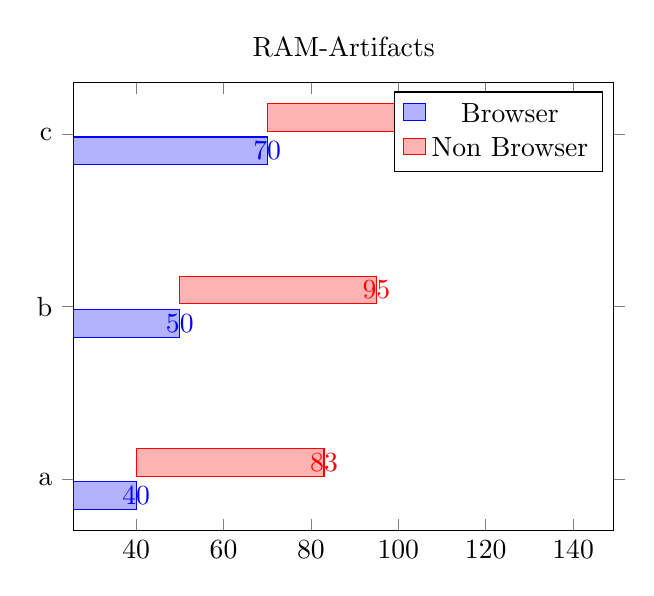
\begin{tikzpicture}
	\begin{axis}[title=RAM-Artifacts,
		xbar,enlargelimits=0.15,nodes near coords,
		symbolic y coords={a,b,c},ytick=data,
		xbar stacked,
		]
		\addplot coordinates
		{(40,a) (50,b) (70,c)};
		\addplot coordinates
		{(43,a) (45,b) (65,c)};
	\legend{Browser, Non Browser}
	\end{axis}
\end{tikzpicture}


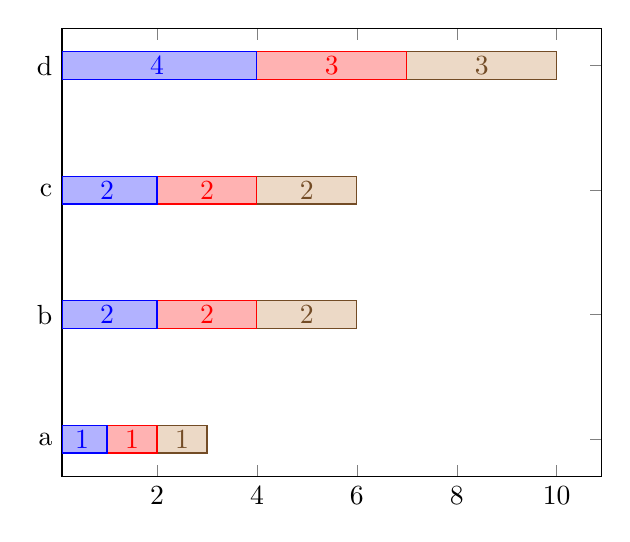
\begin{tikzpicture}
	\begin{axis}[xbar stacked,
		nodes near coords,
		symbolic y coords={a,b,c,d},
		]
		\addplot coordinates
		{(1,a) (2,b) (2,c) (4,d)};
		\addplot coordinates
		{(1,a) (2,b) (2,c) (3,d)};
		\addplot coordinates
		{(1,a) (2,b) (2,c) (3,d)};
	\end{axis}
\end{tikzpicture}

\begin{bchart}[max=8]
	\bcbar[text=A,label=1st label,color=yellow]{6}
	\bcbar[text=B,color=red!50]{3}
	\bcbar[text=C,color=green!60!blue]{4}
	\bcskip{15mm}
	\bcbar[text=D,color=blue]{6}
\end{bchart}

Image + Summary Tabellen hier am Ende no!

\end{comment}

\subsection*{Uncommon Locations}\label{chap:ergebnisse-chrome-uncommon-locations}

Nachfolgend werden die Ergebnisse der Uncommon Location Analyse des Chrome Browsers dargelegt. Dafür werden die beiden Forensik-Programme Autopsy und Volatility verwendet.

\subsubsection*{Analyse mit Autopsy}\label{chap:ergebnisse-chrome-uncommon-autopsy}

Auch in Autopsy konnten keine Artefakte der durchgeführten Browsing-Session gefunden werden, weder durch die Substringsuche, noch durch die Analyse der von Autopsy kategorisierten Dateien. Eine weitergehende Analyse einiger kategorisierter Dateien ist im Anhang \ref{chap:anhang-chrome-uncommon-autopsy} zu finden.

\subsubsection*{Analyse mit Volatility}\label{chap:ergebnisse-chrome-uncommon-volatility}

Nachdem bis jetzt noch keine Artefakte gefunden werden konnten, folgen nun die Analyseergebnisse des Hauptspeichers (RAM), welche mittels des Forensik-Tools Volatility gewonnen wurden. Im RAM konnten schließlich Artefakte gefunden werden. Diese wurden mittels des Volatility Plugins Yarascan identifiziert, wobei die Yara-Regeln aus Anhang \ref{appendix:yara-regeln} verwendet wurden. Zusätzlich zu den erkannten Strings spielt auch noch die PID eine entscheidende Rolle, da damit der Treffer entweder dem Browser oder einem anderen Prozess eindeutig zuordnet werden kann. Die Ergebnisse dieser String-Suche werden nachfolgend präsentiert.

\paragraph*{Yara-Regel \glqq{}HTML\grqq{}}\label{chap:ergebnisse-chrome-uncommon-volatility-html}

Im Gegensatz zu den Ergebnissen der Analyse der beiden vorherigen Browser, konnte ein HTML-Fragment bei Chrome im Arbeitsspeicher gefunden werden. Einzig der String \glqq{}>Themen:\grqq{} wurde im zweiten RAM-Dump in einem Chrome-Prozess gefunden.

%Wie in \autoref{chart:chrome-volatility-htmls} dargestellt, wird der String \glqq{}>Themen:\grqq{} im zweiten RAM-Dump in einem Chrome-Prozess gefunden.
%
%\begin{table}[h!]
%	\resizebox{\linewidth}{!}{
%		\begin{tabular}{r}	
%			\begin{tikzpicture}
%				\begin{axis}[
%					xbar,
%					width=12cm, 
%					height=3cm, 
%					ylabel style={align=center}, ylabel=\textbf{Insiders</span>},
%					y=0.75cm,
%					symbolic y coords={RAM-Dump 3, RAM-Dump 2, RAM-Dump 1},
%					label style={font=\small},
%					tick label style={font=\small},
%					ytick=data,
%					xticklabels={,,},
%					xmin = 0,
%					xmax = 2,
%					nodes near coords, 
%					nodes near coords align={horizontal},
%					nodes near coords style={font=\tiny},
%					nodes near coords={\pgfmathfloatifflags{\pgfplotspointmeta}{0}{}{\pgfmathprintnumber{\pgfplotspointmeta}}},
%					bar width=.17cm,
%					enlarge y limits={abs=2*\pgfplotbarwidth},
%					scaled x ticks=false,
%					legend style={
%						at={(0.5,-0.1)},
%						anchor=north
%					},
%					legend columns=3,
%					yminorgrids = true,minor tick num=1
%					]
%					\addplot coordinates {
%						(0,RAM-Dump 3) (0,RAM-Dump 2) (0,RAM-Dump 1)
%					};
%					\addplot coordinates {
%						(0,RAM-Dump 3) (0,RAM-Dump 2) (0,RAM-Dump 1)
%					};
%				\end{axis}
%			\end{tikzpicture}
%			\\[-7pt]
%			\begin{tikzpicture}
%				\begin{axis}[
%					xbar,
%					width=12cm, 
%					height=3cm, 
%					ylabel style={align=center}, ylabel=\textbf{Ja</span>},
%					y=0.75cm,
%					symbolic y coords={RAM-Dump 3, RAM-Dump 2, RAM-Dump 1},
%					label style={font=\small},
%					tick label style={font=\small},
%					ytick=data,
%					xticklabels={,,},
%					xmin = 0,
%					xmax = 2,
%					nodes near coords, 
%					nodes near coords align={horizontal},
%					nodes near coords style={font=\tiny},
%					nodes near coords={\pgfmathfloatifflags{\pgfplotspointmeta}{0}{}{\pgfmathprintnumber{\pgfplotspointmeta}}},
%					bar width=.17cm,
%					enlarge y limits={abs=2*\pgfplotbarwidth},
%					scaled x ticks=false,
%					legend style={
%						at={(0.5,-0.1)},
%						anchor=north
%					},
%					legend columns=3,
%					yminorgrids = true,minor tick num=1
%					]
%					\addplot coordinates {
%						(0,RAM-Dump 3)  (0,RAM-Dump 2) (0,RAM-Dump 1)
%					};
%					\addplot coordinates {
%						(0,RAM-Dump 3)  (0,RAM-Dump 2) (0,RAM-Dump 1)
%					};
%				\end{axis}
%			\end{tikzpicture}
%			\\[-7pt]
%			\begin{tikzpicture}
%				\begin{axis}[
%					xbar,
%					width=12cm, 
%					height=3cm, 
%					ylabel style={align=center}, ylabel=\textbf{L1</div>},
%					y=0.75cm,
%					symbolic y coords={RAM-Dump 3, RAM-Dump 2, RAM-Dump 1},
%					label style={font=\small},
%					tick label style={font=\small},
%					ytick=data,
%					xticklabels={,,},
%					xmin = 0,
%					xmax = 2,
%					nodes near coords, 
%					nodes near coords align={horizontal},
%					nodes near coords style={font=\tiny},
%					nodes near coords={\pgfmathfloatifflags{\pgfplotspointmeta}{0}{}{\pgfmathprintnumber{\pgfplotspointmeta}}},
%					bar width=.17cm,
%					enlarge y limits={abs=2*\pgfplotbarwidth},
%					scaled x ticks=false,
%					legend style={
%						at={(0.5,-0.1)},
%						anchor=north
%					},
%					legend columns=3,
%					yminorgrids = true,minor tick num=1
%					]
%					\addplot coordinates {
%						(0,RAM-Dump 3)  (0,RAM-Dump 2) (0,RAM-Dump 1)
%					};
%					\addplot coordinates {
%						(0,RAM-Dump 3)  (0,RAM-Dump 2) (0,RAM-Dump 1)
%					};
%				\end{axis}
%			\end{tikzpicture}
%			\\[-7pt]
%			\begin{tikzpicture}
%				\begin{axis}[
%					xbar,
%					width=12cm, 
%					height=3cm, 
%					ylabel style={align=center}, ylabel=\textbf{>Themen:},
%					y=0.75cm,
%					symbolic y coords={RAM-Dump 3, RAM-Dump 2, RAM-Dump 1},
%%					label style={font=\small},
%					tick label style={font=\small},
%					ytick=data,
%					xticklabels={,,},
%					xmin = 0,
%					xmax = 2,
%					nodes near coords, 
%					nodes near coords align={horizontal},
%					nodes near coords style={font=\tiny},
%					nodes near coords={\pgfmathfloatifflags{\pgfplotspointmeta}{0}{}{\pgfmathprintnumber{\pgfplotspointmeta}}},
%					bar width=.17cm,
%					enlarge y limits={abs=2*\pgfplotbarwidth},
%					scaled x ticks=false,
%					legend style={
%						at={(0.5,-0.1)},
%						anchor=north
%					},
%					legend columns=3,
%					yminorgrids = true,minor tick num=1
%					]
%					\addplot coordinates {
%						(0,RAM-Dump 3)  (1,RAM-Dump 2) (0,RAM-Dump 1)
%					};
%					\addplot coordinates {
%						(0,RAM-Dump 3)  (0,RAM-Dump 2) (0,RAM-Dump 1)
%					};
%					\legend{chrome.exe, Andere Prozesse}
%				\end{axis}
%			\end{tikzpicture}
%		\end{tabular}
%	}
%	\caption{Chrome: Anzahl gefundener HTML-Fragmente im RAM}
%	\label{chart:chrome-volatility-htmls}
%\end{table}

Das Volatility-Plugin lieferte hierbei neben dem Treffer noch die PID (7012 in diesem Fall) des Prozesses, in welchem der String gefunden wurde, sowie die virtuelle Adresse, an welchem das Fragment gefunden wurde (0xa6c018187e1). Mit dieser Information wurde dann zunächst der Befehl \texttt{python3 vol.py -f DUMP\_FILE windows.memmap --pid 7012} ausgeführt, um das Memory-Mapping des Prozesses zu erhalten, also die Zuordnung der virtuellen zu den physikalischen Adressen des Prozesses, sowie deren Offset im Memory-Dump-File. In \autoref{tab:chrome-memmap-to-virtual} ist ein Ausschnitt der Ausgabe des Befehls zu sehen.

\begin{table}[h!]
	\centering
	\caption{Chrome: Abbildung virtueller Adressen auf Byte-Offsets der Speicherseite}
	\label{tab:chrome-memmap-to-virtual}
	\resizebox{0.7\linewidth}{!}{
	\begin{tabular}{|l|l|l|l|l|}
	\hline
	\textbf{Virtual}                     & \textbf{Physical}                 & \textbf{Size}                 & \textbf{Offset in File}          & \textbf{File Output}            \\ \hline
	0xa6c01817000                        & 0xc4efc000                        & 0x1000                        & 0x105d000                        & Disabled                        \\ \hline
	{\color[HTML]{FE0000} 0xa6c01818000} & {\color[HTML]{FE0000} 0xd2dfb000} & {\color[HTML]{FE0000} 0x1000} & {\color[HTML]{FE0000} 0x105e000} & {\color[HTML]{FE0000} Disabled} \\ \hline
	0xa6c01819000                        & 0xd50fa000                        & 0x1000                        & 0x105f000                        & Disabled                        \\ \hline
	\end{tabular}
	}
\end{table}

In der Farbe rot ist hervorgehoben, dass die virtuelle Adresse 0xa6c01818000 auf die physikalische Adresse 0xd2dfb000 gemapped ist und der Offset im Memory-File 0x105e000 entspricht. Mithilfe dieser Adressen konnte dann die tatsächliche Position des Strings im Memory-File errechnet werden. Diese betrug somit 0x105e7e1. Anschließend wurde der Speicherbereich des Prozesses als Memory-Dump-File gedumpt und in den Hex-Editor HxD geladen. Dort wurde dann genau an dem errechneten Offset nach dem String gesucht und konnte genau dort auch gefunden werden, was auch in \autoref{pic:ChromeStringThemen} zu sehen ist.
%TODO Evtl doch des andere Bild...

\begin{figure}[h!]
	\centering
	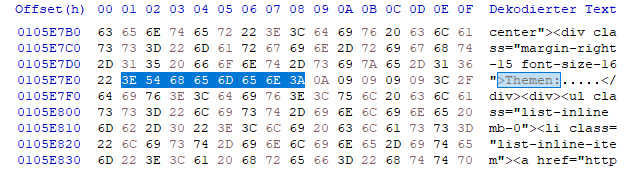
\includegraphics[width=0.75\textwidth]{bilder/HxDChromeStringThemen_cropped.png}
	\caption{Chrome: Ausschnitt aus dem Memory-Dump-File an der Stelle des gefundenen HTML-Strings}
	\label{pic:ChromeStringThemen}
\end{figure} 

Daraufhin wurde weitergehend versucht zu analysieren, ob nur ein Teil der Website im RAM verfügbar ist, oder ob die komplette Donaukurier-Website als HTML-Artefakt im RAM vorhanden ist. Dafür wurde die Internetseite donaukurier.de nochmals aufgerufen, heruntergeladen und der Beginn sowie das Ende der HTML-Datei analysiert. In \autoref{figure:html-begin-end-dk} sind die ersten sowie letzten String-Zeichenketten der HTML-Datei zu sehen.\\


\begin{figure}[!h]
 \begin{minipage}{0.5\textwidth}
  \centering
	\begin{minted}[autogobble=true,frame=single]{html}
	<!DOCTYPE html>
	<html lang="de">
		<head>
		...
	\end{minted}
%  \captionof{subfigure}{Beginn...}
 \end{minipage}
 \begin{minipage}{0.5\textwidth}
  \centering
	\begin{minted}[autogobble=true,frame=single]{html}
			...
	    	</script>
		</body>
	</html>
	\end{minted}
%  \captionof{subfigure}{... und Ende der Donaukurier-Website}
 \end{minipage}
\caption{Chrome: Beginn (links) und Ende (rechts) des HTML-Dokuments der Donaukurier Webseite}
  \label{figure:html-begin-end-dk}
\end{figure}


Davon ausgehend wurde in HxD zuerst nach dem String \glqq{}<!DOCTYPE html>\grqq{} und anschließend nach \glqq{}</html>\grqq{} gesucht. Beide Strings wurden mehrfach in dem Memory-Dump gefunden. Da jedoch keine weiteren Website-typischen Strings mehr durch Yarascan identifiziert werden konnten, wurden die übrigen String-Treffer nicht mehr weiter analysiert.\\
Da bei der Suche des Strings mehr als einen Treffer gab, wurde genau der String ausgewählt, welcher einen niedrigeren Offset als 0x105e7e1 aufweist. In diesem Fall war das der Treffer bei dem Offset von 105201b, was links in \autoref{pic:ChromeBeginDonaukurier} zu sehen ist (markierter Teil). Dabei ist deutlich zu erkennen, dass die Website hier beginnt, da alles Nachfolgende mit dem Beginn der heruntergeladenen Website übereinstimmt und davor nichts im RAM gespeichert wurde.

\begin{figure}[h!]
	\centering
	\subcaptionbox{}{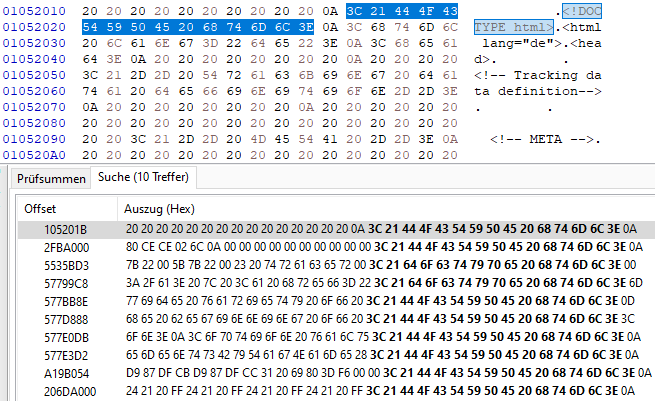
\includegraphics[width=0.47\textwidth]{bilder/HxDChrome1_cropped.png}}%
	\hfill
	\subcaptionbox{}{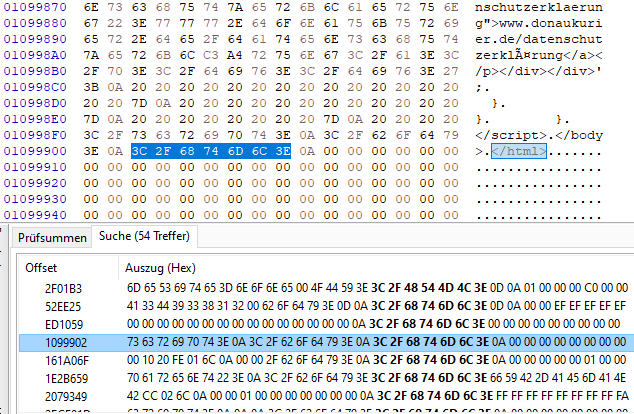
\includegraphics[width=0.47\textwidth]{bilder/HxDChrome3_cropped.png}}%
	\caption{Chrome: Beginn (links) und Ende (rechts) des HTML-Dokuments der Donaukurier Webseite in HxD}
	\label{pic:ChromeBeginDonaukurier}
\end{figure}

Gleiches wurde mit dem Ende der HTML-Datei durchgeführt. \autoref{pic:ChromeBeginDonaukurier} zeigt rechts einen Screenshot mit dem relevanten String-Treffer, welcher das Ende der Website donaukurier.de darstellt.

Anschließend wurde alles, was sich zwischen dem gefundenen Anfang und Ende befindet, als Text kopiert und in eine HTML-Datei gespeichert. Ein detaillierter Vergleich dieses extrahierten Artefakts mit der heruntergeladenen Datei lieferte das Ergebnis, dass die komplette Website rekonstruiert werden kann, die Websiten sich nur in den neuesten Artikeln und Überschriften unterschieden. Übriges war zu 100\% identisch. \\
Zusammenfassend konnte somit die Website \glqq{}donaukurier.de\grqq{} im zweiten Memory-Dump komplett aus dem RAM extrahiert und rekonstruiert werden.

\paragraph*{Yara-Regel \glqq{}Suchbegriffe\grqq{}}\label{chap:ergebnisse-chrome-uncommon-volatility-suchbegriffe}

Wie in Abbildung \ref{chart:chrome-volatility-keywords} dargestellt, wurden die Suchbegriffe \glqq{}pfaffenhofen\grqq{}, \glqq{}nanoradar\grqq{}, \glqq{}mooserliesl\grqq{} und \glqq{}mallofamerica\grqq{} ausschließlich bei dem noch geöffnetem Chrome-Browser nach dem Browsing-Szenario (zweiter RAM-Dump) gefunden. Es wurden dabei alle Suchbegriffe bis auf einen einzigen in Speicherbereichen des Chrome-Browsers gefunden. Am häufigsten konnte der Suchbegriff \glqq{}pfaffenhofen\grqq{} mit 1922 Treffern identifiziert werden. Am seltensten war das der Fall bei dem Begriff \glqq{}mooserliesl\grqq{} mit nur 281 Suchtreffern. \\
Der eine Treffer bei der Suchphrase \glqq{}mallofamerica\grqq{} war im Speicher eines Prozesses mit dem Namen \textit{MemCompression}, was anhand der PID 1828 festgestellt wurde. Dieser Prozess ist dafür zuständig, dass Windows einen Teil des Arbeitsspeichers komprimiert speichert, was zwar zusätzliche CPU-Ressourcen beansprucht, dafür jedoch deutlich schneller ist, als den Hauptspeicher in das pagefile auszulagern \cite{MemCompressionWebsite}. Daher kann es sein, dass ein Teil des RAMs, in welchem der Suchbegriff vorhanden war, komprimiert wurde und folglich dieser Prozess diesen Begriff beinhaltete.

\begin{table}[h!]
	\resizebox{\linewidth}{!}{
		\begin{tabular}{l}	
			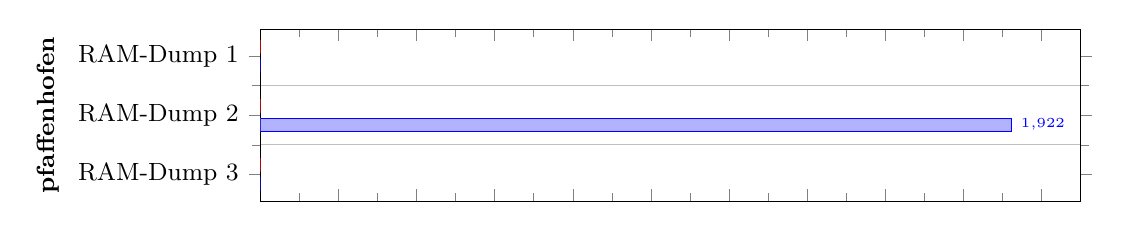
\begin{tikzpicture}
				\begin{axis}[
					xbar,
					width=12cm, 
					height=3cm, 
					ylabel style={align=center}, ylabel=\textbf{pfaffenhofen},
					y=0.75cm,
					symbolic y coords={RAM-Dump 3, RAM-Dump 2, RAM-Dump 1},
					label style={font=\small},
					tick label style={font=\small},
					ytick=data,
					xticklabels={,,},
					xmin = 0,
					xmax = 2100,
					nodes near coords, 
					nodes near coords align={horizontal},
					nodes near coords style={font=\tiny},
					nodes near coords={\pgfmathfloatifflags{\pgfplotspointmeta}{0}{}{\pgfmathprintnumber{\pgfplotspointmeta}}},
					bar width=.17cm,
					enlarge y limits={abs=2*\pgfplotbarwidth},
					scaled x ticks=false,
					legend style={
						at={(0.5,-0.1)},
						anchor=north
					},
					legend columns=3,
					yminorgrids = true,minor tick num=1
					]
					\addplot coordinates {
						(0,RAM-Dump 3) (1922,RAM-Dump 2) (0,RAM-Dump 1)
					};
					\addplot coordinates {
						(0,RAM-Dump 3) (0,RAM-Dump 2) (0,RAM-Dump 1)
					};
				\end{axis}
			\end{tikzpicture}
			\\[-7pt]
			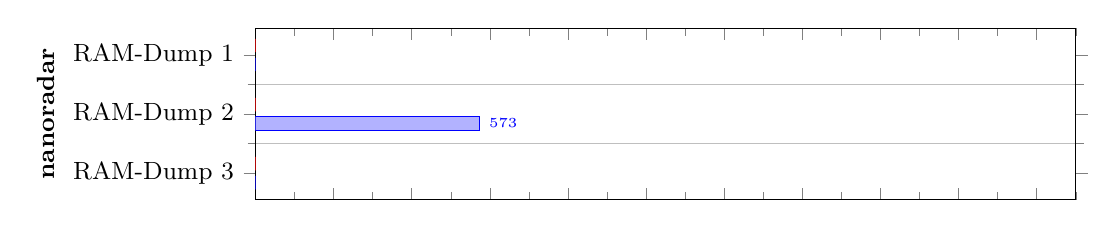
\begin{tikzpicture}
				\begin{axis}[
					xbar,
					width=12cm, 
					height=3cm, 
					ylabel style={align=center}, ylabel=\textbf{nanoradar},
					y=0.75cm,
					symbolic y coords={RAM-Dump 3, RAM-Dump 2, RAM-Dump 1},
					label style={font=\small},
					tick label style={font=\small},
					ytick=data,
					xticklabels={,,},
					xmin = 0,
					xmax = 2100,
					nodes near coords, 
					nodes near coords align={horizontal},
					nodes near coords style={font=\tiny},
					nodes near coords={\pgfmathfloatifflags{\pgfplotspointmeta}{0}{}{\pgfmathprintnumber{\pgfplotspointmeta}}},
					bar width=.17cm,
					enlarge y limits={abs=2*\pgfplotbarwidth},
					scaled x ticks=false,
					legend style={
						at={(0.5,-0.1)},
						anchor=north
					},
					legend columns=3,
					yminorgrids = true,minor tick num=1
					]
					\addplot coordinates {
						(0,RAM-Dump 3)  (573,RAM-Dump 2) (0,RAM-Dump 1)
					};
					\addplot coordinates {
						(0,RAM-Dump 3)  (0,RAM-Dump 2) (0,RAM-Dump 1)
					};
				\end{axis}
			\end{tikzpicture}
			\\[-7pt]
			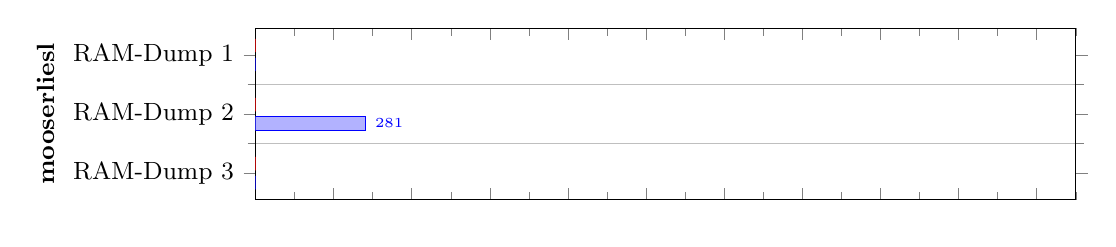
\begin{tikzpicture}
				\begin{axis}[
					xbar,
					width=12cm, 
					height=3cm, 
					ylabel style={align=center}, ylabel=\textbf{mooserliesl},
					y=0.75cm,
					symbolic y coords={RAM-Dump 3, RAM-Dump 2, RAM-Dump 1},
					label style={font=\small},
					tick label style={font=\small},
					ytick=data,
					xticklabels={,,},
					xmin = 0,
					xmax = 2100,
					nodes near coords, 
					nodes near coords align={horizontal},
					nodes near coords style={font=\tiny},
					nodes near coords={\pgfmathfloatifflags{\pgfplotspointmeta}{0}{}{\pgfmathprintnumber{\pgfplotspointmeta}}},
					bar width=.17cm,
					enlarge y limits={abs=2*\pgfplotbarwidth},
					scaled x ticks=false,
					legend style={
						at={(0.5,-0.1)},
						anchor=north
					},
					legend columns=3,
					yminorgrids = true,minor tick num=1
					]
					\addplot coordinates {
						(0,RAM-Dump 3)  (281,RAM-Dump 2) (0,RAM-Dump 1)
					};
					\addplot coordinates {
						(0,RAM-Dump 3)  (0,RAM-Dump 2) (0,RAM-Dump 1)
					};
				\end{axis}
			\end{tikzpicture}
			\\[-7pt]
			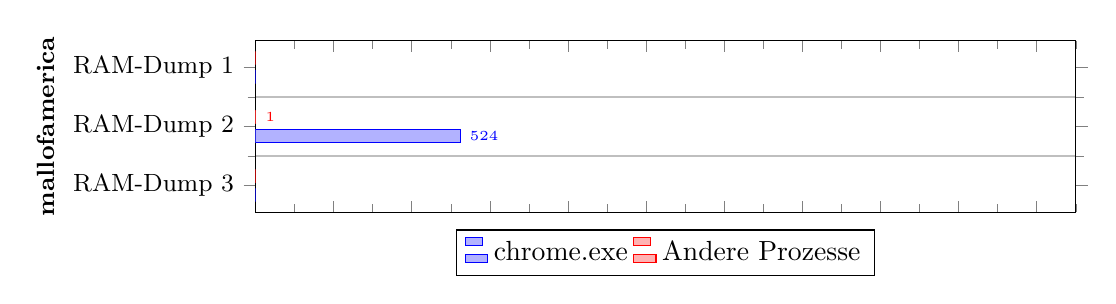
\begin{tikzpicture}
				\begin{axis}[
					xbar,
					width=12cm, 
					height=3cm, 
					ylabel style={align=center}, ylabel=\textbf{mallofamerica},
					y=0.75cm,
					symbolic y coords={RAM-Dump 3, RAM-Dump 2, RAM-Dump 1},
					label style={font=\small},
					tick label style={font=\small},
					ytick=data,
					xticklabels={,,},
					xmin = 0,
					xmax = 2100,
					nodes near coords, 
					nodes near coords align={horizontal},
					nodes near coords style={font=\tiny},
					nodes near coords={\pgfmathfloatifflags{\pgfplotspointmeta}{0}{}{\pgfmathprintnumber{\pgfplotspointmeta}}},
					bar width=.17cm,
					enlarge y limits={abs=2*\pgfplotbarwidth},
					scaled x ticks=false,
					legend style={
						at={(0.5,-0.1)},
						anchor=north
					},
					legend columns=3,
					yminorgrids = true,minor tick num=1
					]
					\addplot coordinates {
						(0,RAM-Dump 3)  (524,RAM-Dump 2) (0,RAM-Dump 1)
					};
					\addplot coordinates {
						(0,RAM-Dump 3)  (1,RAM-Dump 2) (0,RAM-Dump 1)
					};
					\legend{chrome.exe, Andere Prozesse}
				\end{axis}
			\end{tikzpicture}
		\end{tabular}
	}
	\captionof{figure}{Chrome: Anzahl gefundener Suchbegriffe im RAM}
	\label{chart:chrome-volatility-keywords}
\end{table}

\paragraph*{Yara-Regel \glqq{}URLs\grqq{}}\label{chap:ergebnisse-chrome-uncommon-volatility-urls}
Abbildung \ref{chart:chrome-volatility-urls} zeigt, dass in den RAM-Dumps alle Suchbegriffe identifiziert werden konnten. Im ersten Speicherabbild wurden dabei keine URLs gefunden, im zweiten am meisten und im dritten, also nach Beenden des Browsers, konnten auch noch fünf URLs identifiziert werden. Dabei waren es bei der URL \glqq{}donaukurier.com\grqq{} am meisten Suchtreffer mit insgesamt 8157 Treffern, zehn davon waren nicht im Speicher von Chrome-Prozessen zu finden. Zwei davon waren im Prozess \textit{MemCompression}, die restlichen acht wurden im Prozess mit der PID 3760 identifiziert, was in diesem Fall der sihost.exe war. Dieses Programm entspricht dem \textit{Shell Infrastructure Host}, welcher die Grafikbenutzeroberfläche erstellt und verwaltet, wie beispielsweise Desktop-Hintergründe, Popup-Benachrichtigungen und Taskleisten \cite{SiHostWebsite}. Im Prozessbereich dieses Programms befanden sich auch die fünf Treffer aus dem dritten RAM-Dump.

\begin{table}[h!]
	\resizebox{\linewidth}{!}{
		\begin{tabular}{r}	
			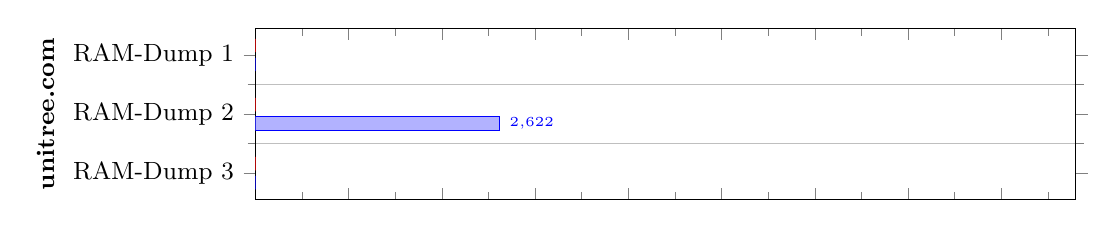
\begin{tikzpicture}
				\begin{axis}[
					xbar,
					width=12cm, 
					height=3cm, 
					ylabel style={align=center}, ylabel=\textbf{unitree.com},
					y=0.75cm,
					symbolic y coords={RAM-Dump 3, RAM-Dump 2, RAM-Dump 1},
					label style={font=\small},
					tick label style={font=\small},
					ytick=data,
					xticklabels={,,},
					xmin = 0,
					xmax = 8800,
					nodes near coords, 
					nodes near coords align={horizontal},
					nodes near coords style={font=\tiny},
					nodes near coords={\pgfmathfloatifflags{\pgfplotspointmeta}{0}{}{\pgfmathprintnumber{\pgfplotspointmeta}}},
					bar width=.17cm,
					enlarge y limits={abs=2*\pgfplotbarwidth},
					scaled x ticks=false,
					legend style={
						at={(0.5,-0.1)},
						anchor=north
					},
					legend columns=3,
					yminorgrids = true,minor tick num=1
					]
					\addplot coordinates {
						(0,RAM-Dump 3) (2622,RAM-Dump 2) (0,RAM-Dump 1)
					};
					\addplot coordinates {
						(0,RAM-Dump 3) (0,RAM-Dump 2) (0,RAM-Dump 1)
					};
				\end{axis}
			\end{tikzpicture}
			\\[-7pt]
			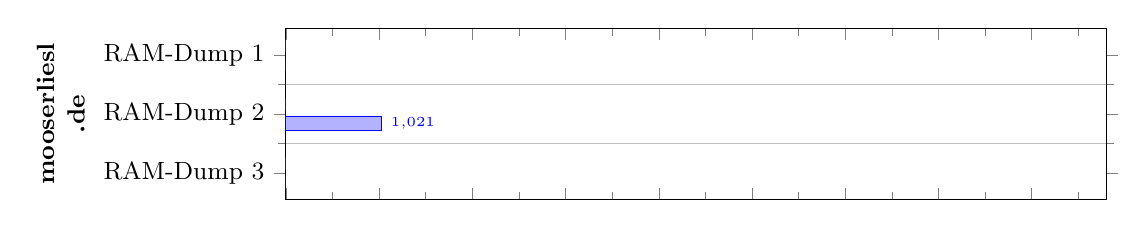
\begin{tikzpicture}
				\begin{axis}[
					xbar,
					width=12cm, 
					height=3cm, 
					ylabel style={align=center}, ylabel=\textbf{mooserliesl}\\\textbf{.de},
					y=0.75cm,
					symbolic y coords={RAM-Dump 3, RAM-Dump 2, RAM-Dump 1},
					label style={font=\small},
					tick label style={font=\small},
					ytick=data,
					xticklabels={,,},
					xmin = 0,
					xmax = 8800,
					nodes near coords, 
					nodes near coords align={horizontal},
					nodes near coords style={font=\tiny},
					nodes near coords={\pgfmathfloatifflags{\pgfplotspointmeta}{0}{}{\pgfmathprintnumber{\pgfplotspointmeta}}},
					bar width=.17cm,
					enlarge y limits={abs=2*\pgfplotbarwidth},
					scaled x ticks=false,
					legend style={
						at={(0.5,-0.1)},
						anchor=north
					},
					legend columns=3,
					yminorgrids = true,minor tick num=1
					]
					\addplot coordinates {
						(0,RAM-Dump 3) (1021,RAM-Dump 2) (0,RAM-Dump 1)
					};
					\addplot coordinates {
						(0,RAM-Dump 3) (0,RAM-Dump 2) (0,RAM-Dump 1)
					};
				\end{axis}
			\end{tikzpicture}	
			\\[-7pt]
			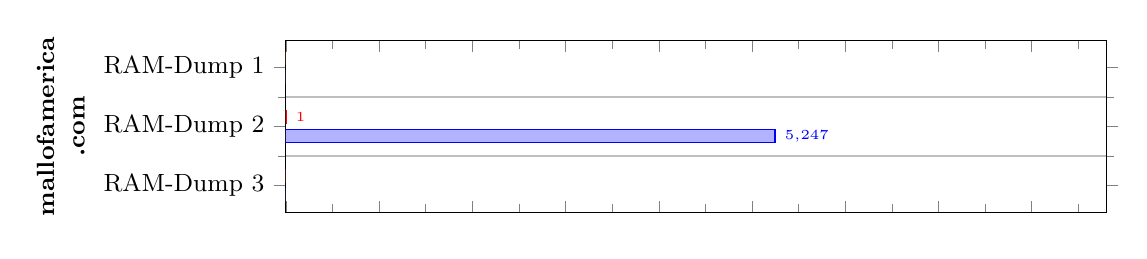
\begin{tikzpicture}
				\begin{axis}[
					xbar,
					width=12cm, 
					height=3cm, 
					ylabel style={align=center}, ylabel=\textbf{mallofamerica}\\\textbf{.com},
					y=0.75cm,
					symbolic y coords={RAM-Dump 3, RAM-Dump 2, RAM-Dump 1},
					label style={font=\small},
					tick label style={font=\small},
					ytick=data,
					xticklabels={,,},
					xmin = 0,
					xmax = 8800,
					nodes near coords, 
					nodes near coords align={horizontal},
					nodes near coords style={font=\tiny},
					nodes near coords={\pgfmathfloatifflags{\pgfplotspointmeta}{0}{}{\pgfmathprintnumber{\pgfplotspointmeta}}},
					bar width=.17cm,
					enlarge y limits={abs=2*\pgfplotbarwidth},
					scaled x ticks=false,
					legend style={
						at={(0.5,-0.1)},
						anchor=north
					},
					legend columns=3,
					yminorgrids = true,minor tick num=1
					]
					\addplot coordinates {
						(0,RAM-Dump 3) (5247,RAM-Dump 2) (0,RAM-Dump 1)
					};
					\addplot coordinates {
						(0,RAM-Dump 3) (1,RAM-Dump 2) (0,RAM-Dump 1)
					};
				\end{axis}
			\end{tikzpicture}
			\\[-7pt]
			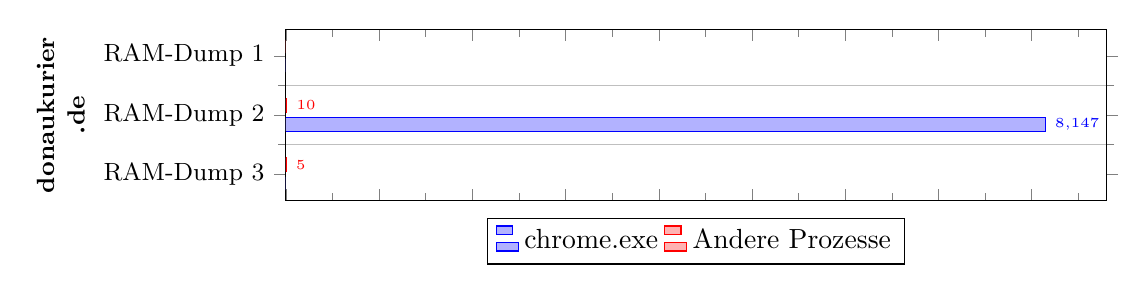
\begin{tikzpicture}
				\begin{axis}[
					xbar,
					width=12cm, 
					height=3cm, 
					ylabel style={align=center}, ylabel=\textbf{donaukurier}\\\textbf{.de},
					y=0.75cm,
					symbolic y coords={RAM-Dump 3, RAM-Dump 2, RAM-Dump 1},
					label style={font=\small},
					tick label style={font=\small},
					ytick=data,
					xticklabels={,,},
					xmin = 0,
					xmax = 8800,
					nodes near coords, 
					nodes near coords align={horizontal},
					nodes near coords style={font=\tiny},
					nodes near coords={\pgfmathfloatifflags{\pgfplotspointmeta}{0}{}{\pgfmathprintnumber{\pgfplotspointmeta}}},
					bar width=.17cm,
					enlarge y limits={abs=2*\pgfplotbarwidth},
					scaled x ticks=false,
					legend style={
						at={(0.5,-0.1)},
						anchor=north
					},
					legend columns=3,
					yminorgrids = true,minor tick num=1
					]
					\addplot coordinates {
						(0,RAM-Dump 3) (8147,RAM-Dump 2) (0,RAM-Dump 1)
					};
					\addplot coordinates {
						(5,RAM-Dump 3) (10,RAM-Dump 2) (0,RAM-Dump 1)
					};
					\legend{chrome.exe, Andere Prozesse}
				\end{axis}
			\end{tikzpicture}		
		\end{tabular}
	}
	\captionof{figure}{Chrome: Anzahl gefundener URLs im RAM}
	\label{chart:chrome-volatility-urls}
\end{table}

\paragraph*{Yara-Regel \glqq{}E-Mail\grqq{}}\label{chap:ergebnisse-chrome-uncommon-volatility-email}
Wie in Abbildung \ref{chart:chrome-volatility-mail} gezeigt, wurden sowohl nach dem Browsing-Szenario bei geöffnetem Browser, als auch nach Schließen desselben E-Mail Artefakte gefunden. Darunter war die E-Mail-Adresse mit 172 Treffern, acht davon außerhalb von Chrome-Prozessen, das häufigste Suchresultat. Unter den acht externen Prozessen waren der \textit{Desktop Window Manager}, welcher für visuelle Effekte wie Desktop-Animationen und halbtransparente Fenster verantwortlich ist \cite{dwmWebsite}, explorer.exe, sihost.exe und weiteren Windows-Prozessen. Da dies aber meist Window-Manager-Prozesse waren, wurden diese nicht weiter analysiert. \\
Die beiden Studenten-Mailadressen, an welche die Mail versendet wurden, waren mit 121 bzw. 97 Suchtreffern in Chrome-Prozessen vertreten. Der Mailtext war mit 136 Artefakten mehr als doppelt so oft im RAM zu finden als der Betrefftext. Im dritten RAM-Dump wurde dann noch die E-Mail-Adresse im Prozess \textit{explorer.exe} gefunden.\\
Grundsätzlich wurden bei dieser Yara-Regel wenige Artefakte identifiziert im Vergleich zu den URLs beispielsweise.


\begin{table}[h!]
	\resizebox{\linewidth}{!}{
		\begin{tabular}{r}	
			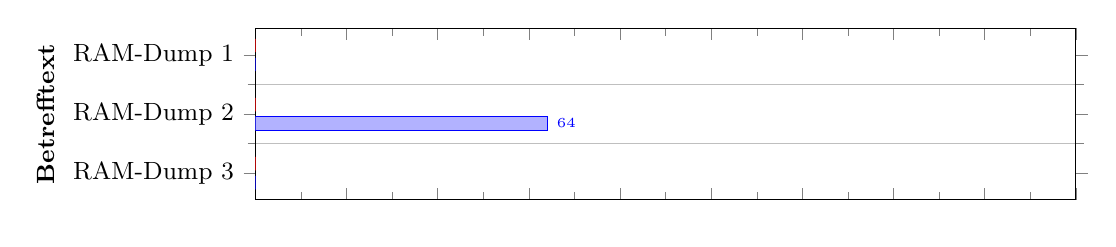
\begin{tikzpicture}
				\begin{axis}[
					xbar,
					width=12cm, 
					height=3cm, 
					ylabel style={align=center}, ylabel=\textbf{Betrefftext},
					y=0.75cm,
					symbolic y coords={RAM-Dump 3, RAM-Dump 2, RAM-Dump 1},
					label style={font=\small},
					tick label style={font=\small},
					ytick=data,
					xticklabels={,,},
					xmin = 0,
					xmax = 180,
					nodes near coords, 
					nodes near coords align={horizontal},
					nodes near coords style={font=\tiny},
					nodes near coords={\pgfmathfloatifflags{\pgfplotspointmeta}{0}{}{\pgfmathprintnumber{\pgfplotspointmeta}}},
					bar width=.17cm,
					enlarge y limits={abs=2*\pgfplotbarwidth},
					scaled x ticks=false,
					legend style={
						at={(0.5,-0.1)},
						anchor=north
					},
					legend columns=3,
					yminorgrids = true,minor tick num=1
					]
					\addplot coordinates {
						(0,RAM-Dump 3) (64,RAM-Dump 2) (0,RAM-Dump 1)
					};
					\addplot coordinates {
						(0,RAM-Dump 3) (0,RAM-Dump 2) (0,RAM-Dump 1)
					};
					%				\legend{firefox.exe, Andere Prozesse}
				\end{axis}
			\end{tikzpicture}
			\\[-7pt]
			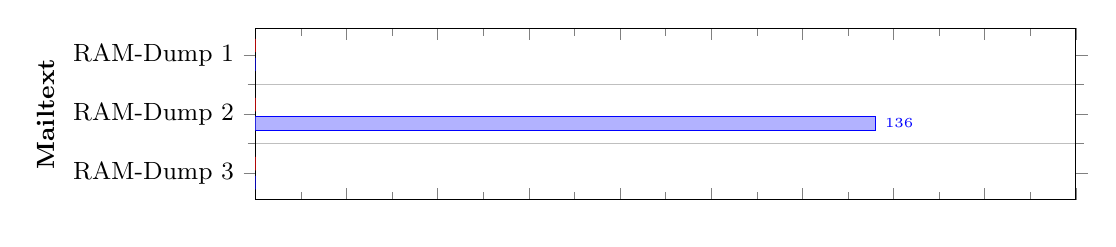
\begin{tikzpicture}
				\begin{axis}[
					xbar,
					width=12cm, 
					height=3cm, 
					ylabel style={align=center}, ylabel=\textbf{Mailtext},
					y=0.75cm,
					symbolic y coords={RAM-Dump 3, RAM-Dump 2, RAM-Dump 1},
					label style={font=\small},
					tick label style={font=\small},
					ytick=data,
					xticklabels={,,},
					xmin = 0,
					xmax = 180,
					nodes near coords, 
					nodes near coords align={horizontal},
					nodes near coords style={font=\tiny},
					nodes near coords={\pgfmathfloatifflags{\pgfplotspointmeta}{0}{}{\pgfmathprintnumber{\pgfplotspointmeta}}},
					bar width=.17cm,
					enlarge y limits={abs=2*\pgfplotbarwidth},
					scaled x ticks=false,
					legend style={
						at={(0.5,-0.1)},
						anchor=north
					},
					legend columns=3,
					yminorgrids = true,minor tick num=1
					]
					\addplot coordinates {
						(0,RAM-Dump 3) (136,RAM-Dump 2) (0,RAM-Dump 1)
					};
					\addplot coordinates {
						(0,RAM-Dump 3) (0,RAM-Dump 2) (0,RAM-Dump 1)
					};
					%				\legend{firefox.exe, Andere Prozesse}
				\end{axis}
			\end{tikzpicture}	
			\\[-7pt]
			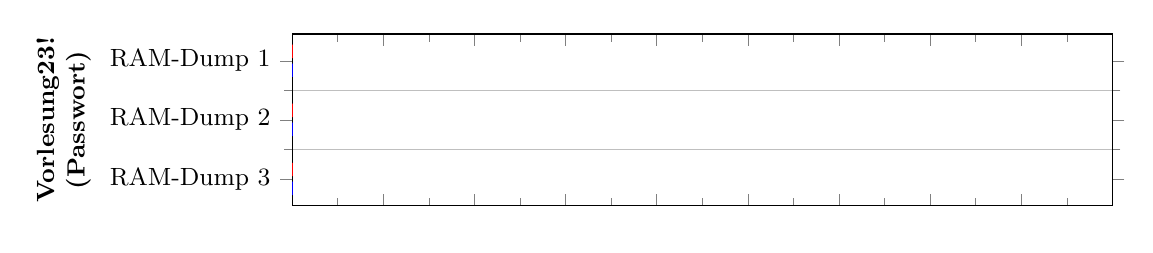
\begin{tikzpicture}
				\begin{axis}[
					xbar,
					width=12cm, 
					height=3cm, 
					ylabel style={align=center}, ylabel=\textbf{Vorlesung23!}\\\textbf{(Passwort)},
					y=0.75cm,
					symbolic y coords={RAM-Dump 3, RAM-Dump 2, RAM-Dump 1},
					label style={font=\small},
					tick label style={font=\small},
					ytick=data,
					xticklabels={,,},
					xmin = 0,
					xmax = 180,
					nodes near coords, 
					nodes near coords align={horizontal},
					nodes near coords style={font=\tiny},
					nodes near coords={\pgfmathfloatifflags{\pgfplotspointmeta}{0}{}{\pgfmathprintnumber{\pgfplotspointmeta}}},
					bar width=.17cm,
					enlarge y limits={abs=2*\pgfplotbarwidth},
					scaled x ticks=false,
					legend style={
						at={(0.5,-0.1)},
						anchor=north
					},
					legend columns=3,
					yminorgrids = true,minor tick num=1
					]
					\addplot coordinates {
						(0,RAM-Dump 3) (0,RAM-Dump 2) (0,RAM-Dump 1)
					};
					\addplot coordinates {
						(0,RAM-Dump 3) (0,RAM-Dump 2) (0,RAM-Dump 1)
					};
					%				\legend{firefox.exe, Andere Prozesse}
				\end{axis}
			\end{tikzpicture}
			\\[-7pt]
			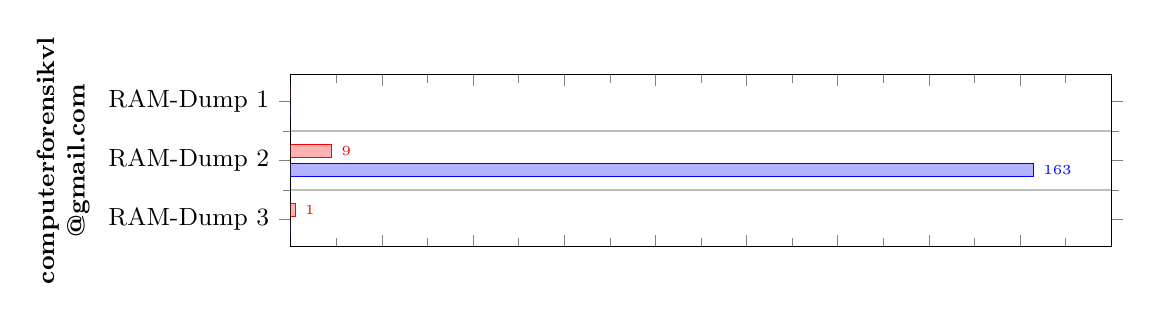
\begin{tikzpicture}
				\begin{axis}[
					xbar,
					width=12cm, 
					height=3cm, 
					ylabel style={align=center}, ylabel=\textbf{computerforensikvl}\\\textbf{@gmail.com},
					y=0.75cm,
					symbolic y coords={RAM-Dump 3, RAM-Dump 2, RAM-Dump 1},
					label style={font=\small},
					tick label style={font=\small},
					ytick=data,
					xticklabels={,,},
					xmin = 0,
					xmax = 180,
					nodes near coords, 
					nodes near coords align={horizontal},
					nodes near coords style={font=\tiny},
					nodes near coords={\pgfmathfloatifflags{\pgfplotspointmeta}{0}{}{\pgfmathprintnumber{\pgfplotspointmeta}}},
					bar width=.17cm,
					enlarge y limits={abs=2*\pgfplotbarwidth},
					scaled x ticks=false,
					legend style={
						at={(0.5,-0.1)},
						anchor=north
					},
					legend columns=3,
					yminorgrids = true,minor tick num=1
					]
					\addplot coordinates {
						(0,RAM-Dump 3) (163,RAM-Dump 2) (0,RAM-Dump 1)
					};
					\addplot coordinates {
						(1,RAM-Dump 3) (9,RAM-Dump 2) (0,RAM-Dump 1)
					};
					%				\legend{firefox.exe, Andere Prozesse}
				\end{axis}
			\end{tikzpicture}	
			\\[-7pt]
			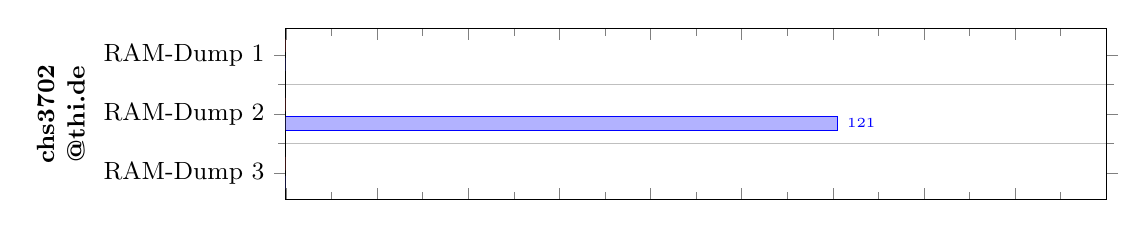
\begin{tikzpicture}
				\begin{axis}[
					xbar,
					width=12cm, 
					height=3cm, 
					ylabel style={align=center}, ylabel=\textbf{chs3702}\\\textbf{@thi.de},
					y=0.75cm,
					symbolic y coords={RAM-Dump 3, RAM-Dump 2, RAM-Dump 1},
					label style={font=\small},
					tick label style={font=\small},
					ytick=data,
					xticklabels={,,},
					xmin = 0,
					xmax = 180,
					nodes near coords, 
					nodes near coords align={horizontal},
					nodes near coords style={font=\tiny},
					nodes near coords={\pgfmathfloatifflags{\pgfplotspointmeta}{0}{}{\pgfmathprintnumber{\pgfplotspointmeta}}},
					bar width=.17cm,
					enlarge y limits={abs=2*\pgfplotbarwidth},
					scaled x ticks=false,
					legend style={
						at={(0.5,-0.1)},
						anchor=north
					},
					legend columns=3,
					yminorgrids = true,minor tick num=1
					]
					\addplot coordinates {
						(0,RAM-Dump 3) (121,RAM-Dump 2) (0,RAM-Dump 1)
					};
					\addplot coordinates {
						(0,RAM-Dump 3) (0,RAM-Dump 2) (0,RAM-Dump 1)
					};
					%				\legend{firefox.exe, Andere Prozesse}
				\end{axis}
			\end{tikzpicture}
			\\[-7pt]
			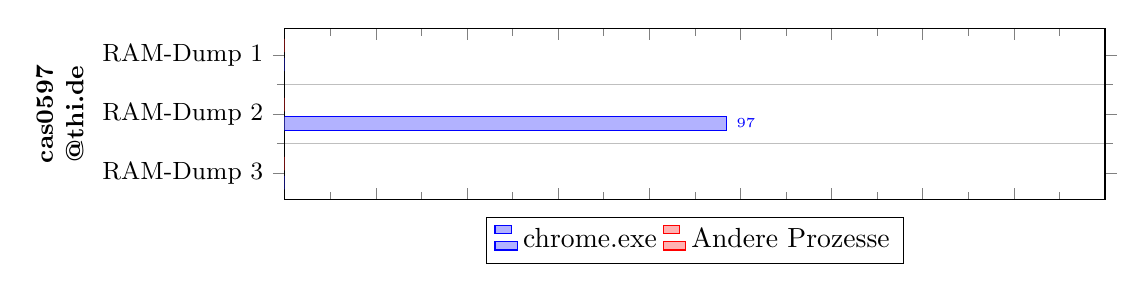
\begin{tikzpicture}
				\begin{axis}[
					xbar,
					width=12cm, 
					height=3cm, 
					ylabel style={align=center}, ylabel=\textbf{cas0597}\\\textbf{@thi.de},
					y=0.75cm,
					symbolic y coords={RAM-Dump 3, RAM-Dump 2, RAM-Dump 1},
					label style={font=\small},
					tick label style={font=\small},
					ytick=data,
					xticklabels={,,},
					xmin = 0,
					xmax = 180,
					nodes near coords, 
					nodes near coords align={horizontal},
					nodes near coords style={font=\tiny},
					nodes near coords={\pgfmathfloatifflags{\pgfplotspointmeta}{0}{}{\pgfmathprintnumber{\pgfplotspointmeta}}},
					bar width=.17cm,
					enlarge y limits={abs=2*\pgfplotbarwidth},
					scaled x ticks=false,
					legend style={
						at={(0.5,-0.1)},
						anchor=north
					},
					legend columns=3,
					yminorgrids = true,minor tick num=1
					]
					\addplot coordinates {
						(0,RAM-Dump 3) (97,RAM-Dump 2) (0,RAM-Dump 1)
					};
					\addplot coordinates {
						(0,RAM-Dump 3) (0,RAM-Dump 2) (0,RAM-Dump 1)
					};
					\legend{chrome.exe, Andere Prozesse}
				\end{axis}
			\end{tikzpicture}
			%	\begin{axis}[]
				%	\legend{Logfile 1, Logfile 2}
				%	\end{axis}
			
		\end{tabular}
	}
	\captionof{figure}{Chrome: Anzahl gefundener E-Mail Artefakte im RAM}
	\label{chart:chrome-volatility-mail}
\end{table}

\paragraph{Yara-Regel \glqq{}DK-Logo\grqq{}}\label{chap:ergebnisse-chrome-uncommon-volatility-dklogo}

Bei der letzten Yara-Regel zeigt Abbildung \ref{chart:chrome-volatility-image} die Ergebnisse, in welchem RAM-Dump und wie oft das Donaukurier Logo im RAM identifiziert werden konnte. Zu sehen ist, dass dies nur im zweiten Speicherabbild der Fall war und insgesamt dreimal dort in einem Chrome-Prozess zu finden war.

\begin{table}[h!]
	\resizebox{\linewidth}{!}{
		\begin{tabular}{r}
			\begin{tikzpicture}
				\begin{axis}[
					xbar stacked,
					width=18cm, 
					height=12cm, 
					ylabel style={align=center}, ylabel=Donaukurier Logo\\(Hexadezimal),
					y=1cm,
					symbolic y coords={RAM-Dump 3, RAM-Dump 2, RAM-Dump 1},
					ytick=data,
					xticklabels={,,},
					xmin = 0,
					xmax = 4,
					nodes near coords, 
					nodes near coords align={horizontal},
					legend style={
						at={(0.5,-0.1)},
						anchor=north
					},
					legend columns=2
					]
					\addplot coordinates {
						(0,RAM-Dump 3) (3,RAM-Dump 2) (0,RAM-Dump 1)
					};
					\addplot coordinates {
						(0,RAM-Dump 3) (0,RAM-Dump 2) (0,RAM-Dump 1)
					};
					\legend{chrome.exe, Andere Prozesse}
				\end{axis}
			\end{tikzpicture}
		\end{tabular}
	}
	\captionof{figure}{Chrome: Anzahl gefundener Hexadezimalwerte des Donaukurier-Logos im RAM}
	\label{chart:chrome-volatility-image}
\end{table}

\subsection*{Registry}\label{chap:ergebnisse-chrome-uncommon-registry}

Wie in \autoref{subsection:methodik-datenanalyse-registry} beschrieben, zählt die Analyse der Registry sowohl zu den Common als auch zu den Uncommon Locations. Es können weder in den \glqq{}SetValue\grqq{}-Operationen in den Process Monitor Logs noch durch die Analyse der System- und User-Hives durch den RegistryExplorer Artefakte gefunden werden. Eine weitergehende Analyse der Registry ist im Anhang \ref{chap:anhang-chrome-registry} beschrieben.
% Aufführen aller Registry-Schreiboperationen, wie analysiert, 

\pagebreak
\section{Brave}\label{chap:ergebnisse-brave}

\begin{comment}

Analyse aller Schreiboperationen mittels des ProcessMonitors:

2 Logs aufgezeichnet gemäß [link], Analyse in getrennten Kapiteln

\subsubsection*{Process Monitor Log 1}

Unterschieden in bekannte Browser-Pfade (Browser-Pfad) und andere Pfade (außerhalb des typischen Browser-Pfades)

Bekannt:

Glob gegliedert in Dateiendungen, mit möglichen Erklärungen: \\
\begin{comment}
- 000003.log's:  \\
- tmp \\
- png \\
- store\_new \\
- .Identifier \\
- .db  \\
- LOG \\
- .pb \\
- .ftlite \\
- .dbtemp \\
- others -> Erklärung der Datenbanken + locations

=> Zusammenfassung in Tabelle \\\\

Unbekannter Pfad:\\
- tmp files, nicht mehr auffindbar\\
- 


Alle Schreiboperationen mit aufnehmen in Anhang evtl.

\subsubsection*{Process Monitor Log 2}

Hier Erklärungen zu 2. mit Tabelle rein

\subsubsection*{Databases}

Welche Datenbanken sind wann vorhanden? Was verändert sich über die Zeit? Textuell + Tabellarisch zeigen!

\subsection*{Registry}

\subsubsection*{Process Monitor}

Zuerst die im Process Monitor aufgeze

\subsubsection*{Hives-Extraction inklusive Analyse}

Dann Auslesen der bereits in [link] dargestellten Hives + Einlesen in Registry Explorer. Liefert bei allen 3 betrachteten Snapshots keine Ergebnisse

\subsection*{Black-Box Analyse/Uncommon Locations}

\subsubsection*{Analyse mit Autopsy}

\subsubsection*{Analyse mit Volatility}

Jeweils schöne Tabellen hierzu:

Keywords\\
URL\\
Mail \\
HTTP inkl. Screenshots hier (Verweis nach oben)

Image + Summary Tabellen hier am Ende no!

\end{comment}

Abschließend werden in diesem Kapitel die Analyseergebnisse des Browsers Brave dargelegt, wobei diese wieder, wie in den vorherigen Kapiteln, in Common Locations, Uncommon Locations und der Registry unterteilt werden.

\subsection*{Common Locations}\label{chap:ergebnisse-brave-common-locations}

Zu Beginn erfolgt die Untersuchung der Common Locations auf potenzielle private Browsing-Artefakte. Bei der Analyse der Schreiboperationen aus den Process Monitor Logfiles konnten keine Artefakte befunden werden, wie es auch bei der Untersuchung der SQLite-Datenbanken der Fall war.\\
Eine umfangreiche Auswertung der Daten sowie den Datenbanken befindet sich im Anhang \ref{chap:anhang-brave-common-locations}.

\subsection*{Uncommon Locations}\label{chap:ergebnisse-brave-uncommon-locations}

Anschließend an die Common Locations folgt nun die Untersuchung der Uncommon Locations. Dafür werden vollständige Speicherabbilder nach Artefakten der privaten Browsing-Session untersucht. Für diesen Zweck werden die beiden Forensik-Programme Autopsy und Volatility verwendet.

\subsubsection*{Analyse mit Autopsy}\label{chap:ergebnisse-brave-uncommon-locations-autopsy}

Autopsy wird bei den Uncommon Locations zusätzlich als forensisches Werkzeug verwendet im Gegensatz zur Analyse der Common Locations, bei welchen es eingesetzt wurde, um Dateien aus den Snapshots zu extrahieren.\\
Zunächst wurde die Stringsuche gemäß \autoref{subsubsection:methodik-datenanalyse-uncommonlocations-analysemitautopsy} eingesetzt, wobei es keine Suchtreffer gab.\\
Zusätzlich wurden automatisch kategorisierte Dateien untersucht, wobei hier auch keine Artefakte zu finden waren. Anhang \ref{chap:anhang-brave-uncommon-locations-autopsy} geht auf diese Dateien ausführlicher ein.

\subsubsection*{Analyse mit Volatility}\label{chap:ergebnisse-brave-uncommon-locations-volatility}

Für die Analyse des Arbeitsspeichers wurde das Forensik-Tool Volatility verwendet, womit eine Stringsuche mittels des Plugins Yarascan durchgeführt wird. Damit durchsucht man ein Arbeitsspeicherabbild nach gewissen String-Mustern, welche zuvor in einer Yara-Regel festgelegt werden können. Die für diese Arbeit verwendete Datei inklusive der Regeln ist in Anhang \ref{appendix:yara-regeln} aufgeführt. 

\paragraph*{Yara-Regel \glqq{}HTML\grqq{}}\label{chap:ergebnisse-brave-uncommon-locations-volatility-html}

Beim Brave-Browser konnte ausschließlich ein HTML-Fragment im zweiten RAM-Dump wiederhergestellt werden. Dabei handelt es sich wie bei Chrome um den String \glqq{}>Themen:\grqq.

%\begin{table}[h!]
%	\resizebox{\linewidth}{!}{
%		\begin{tabular}{l}	
%			\begin{tikzpicture}
%				\begin{axis}[
%					xbar,
%					width=12cm, 
%					height=3cm, 
%					ylabel style={align=center}, ylabel=\textbf{Insiders</span>},
%					y=0.75cm,
%					symbolic y coords={RAM-Dump 3, RAM-Dump 2, RAM-Dump 1},
%					label style={font=\small},
%					tick label style={font=\small},
%					ytick=data,
%					xticklabels={,,},
%					xmin = 0,
%					xmax = 2,
%					nodes near coords, 
%					nodes near coords align={horizontal},
%					nodes near coords style={font=\tiny},
%					nodes near coords={\pgfmathfloatifflags{\pgfplotspointmeta}{0}{}{\pgfmathprintnumber{\pgfplotspointmeta}}},
%					bar width=.17cm,
%					enlarge y limits={abs=2*\pgfplotbarwidth},
%					scaled x ticks=false,
%					legend style={
%						at={(0.5,-0.1)},
%						anchor=north
%					},
%					legend columns=3,
%					yminorgrids = true,minor tick num=1
%					]
%					\addplot coordinates {
%						(0,RAM-Dump 3) (0,RAM-Dump 2) (0,RAM-Dump 1)
%					};
%					\addplot coordinates {
%						(0,RAM-Dump 3) (0,RAM-Dump 2) (0,RAM-Dump 1)
%					};
%				\end{axis}
%			\end{tikzpicture}
%			\\[-7pt]
%			\begin{tikzpicture}
%				\begin{axis}[
%					xbar,
%					width=12cm, 
%					height=3cm, 
%					ylabel style={align=center}, ylabel=\textbf{Ja</span>},
%					y=0.75cm,
%					symbolic y coords={RAM-Dump 3, RAM-Dump 2, RAM-Dump 1},
%					label style={font=\small},
%					tick label style={font=\small},
%					ytick=data,
%					xticklabels={,,},
%					xmin = 0,
%					xmax = 2,
%					nodes near coords, 
%					nodes near coords align={horizontal},
%					nodes near coords style={font=\tiny},
%					nodes near coords={\pgfmathfloatifflags{\pgfplotspointmeta}{0}{}{\pgfmathprintnumber{\pgfplotspointmeta}}},
%					bar width=.17cm,
%					enlarge y limits={abs=2*\pgfplotbarwidth},
%					scaled x ticks=false,
%					legend style={
%						at={(0.5,-0.1)},
%						anchor=north
%					},
%					legend columns=3,
%					yminorgrids = true,minor tick num=1
%					]
%					\addplot coordinates {
%						(0,RAM-Dump 3)  (0,RAM-Dump 2) (0,RAM-Dump 1)
%					};
%					\addplot coordinates {
%						(0,RAM-Dump 3)  (0,RAM-Dump 2) (0,RAM-Dump 1)
%					};
%				\end{axis}
%			\end{tikzpicture}
%			\\[-7pt]
%			\begin{tikzpicture}
%				\begin{axis}[
%					xbar,
%					width=12cm, 
%					height=3cm, 
%					ylabel style={align=center}, ylabel=\textbf{L1</div>},
%					y=0.75cm,
%					symbolic y coords={RAM-Dump 3, RAM-Dump 2, RAM-Dump 1},
%					label style={font=\small},
%					tick label style={font=\small},
%					ytick=data,
%					xticklabels={,,},
%					xmin = 0,
%					xmax = 2,
%					nodes near coords, 
%					nodes near coords align={horizontal},
%					nodes near coords style={font=\tiny},
%					nodes near coords={\pgfmathfloatifflags{\pgfplotspointmeta}{0}{}{\pgfmathprintnumber{\pgfplotspointmeta}}},
%					bar width=.17cm,
%					enlarge y limits={abs=2*\pgfplotbarwidth},
%					scaled x ticks=false,
%					legend style={
%						at={(0.5,-0.1)},
%						anchor=north
%					},
%					legend columns=3,
%					yminorgrids = true,minor tick num=1
%					]
%					\addplot coordinates {
%						(0,RAM-Dump 3)  (0,RAM-Dump 2) (0,RAM-Dump 1)
%					};
%					\addplot coordinates {
%						(0,RAM-Dump 3)  (0,RAM-Dump 2) (0,RAM-Dump 1)
%					};
%				\end{axis}
%			\end{tikzpicture}
%			\\[-7pt]
%			\begin{tikzpicture}
%				\begin{axis}[
%					xbar,
%					width=12cm, 
%					height=3cm, 
%					ylabel style={align=center}, ylabel=\textbf{>Themen:},
%					y=0.75cm,
%					symbolic y coords={RAM-Dump 3, RAM-Dump 2, RAM-Dump 1},
%%					label style={font=\small},
%					tick label style={font=\small},
%					ytick=data,
%					xticklabels={,,},
%					xmin = 0,
%					xmax = 2,
%					nodes near coords, 
%					nodes near coords align={horizontal},
%					nodes near coords style={font=\tiny},
%					nodes near coords={\pgfmathfloatifflags{\pgfplotspointmeta}{0}{}{\pgfmathprintnumber{\pgfplotspointmeta}}},
%					bar width=.17cm,
%					enlarge y limits={abs=2*\pgfplotbarwidth},
%					scaled x ticks=false,
%					legend style={
%						at={(0.5,-0.1)},
%						anchor=north
%					},
%					legend columns=3,
%					yminorgrids = true,minor tick num=1
%					]
%					\addplot coordinates {
%						(0,RAM-Dump 3)  (1,RAM-Dump 2) (0,RAM-Dump 1)
%					};
%					\addplot coordinates {
%						(0,RAM-Dump 3)  (0,RAM-Dump 2) (0,RAM-Dump 1)
%					};
%					\legend{brave.exe, Andere Prozesse}
%				\end{axis}
%			\end{tikzpicture}
%		\end{tabular}
%	}
%	\caption{Brave: Anzahl gefundener HTML-Fragmente im RAM}
%	\label{chart:brave-volatility-htmls}
%\end{table}

Die Extraktion der kompletten Webseite war dabei wie in \autoref{chap:ergebnisse-chrome-uncommon-volatility-html} möglich. Auch das Vorgehen war identisch, außer, wie zu erwarten war, die virtuellen und physikalischen Adressen der verschiedenen Zeichenketten. Daher wird hier nicht nochmal ausführlich auf das Vorgehen der Extraktion der Webseite aufgeführt.\\
Anschließend an die Wiederherstellung der HTML-Datei wurden die beiden extrahierten Dateien nochmals gegeneinander verglichen. \autoref{pic:compareHTMLs} zeigt dies anhand der \textit{compare}-Funktionalität von Visual Studio Code. An der rechten Seite in der Bildlaufleiste sind die Sektionen farbig dargestellt, welche Unterschiede aufweisen. Dabei wurde durch Analyse derer deutlich, dass der Aufbau und die Struktur beider extrahierter Webseiten übereinstimmt, es nur geringe Unterschiede bei einigen Namen der Artikel und Meldungen gibt. Die Dateien sind nahezu identisch groß (290kB).
%\autoref{pic:brave-vimdiff} zeigt einen Ausschnitt eines generierten HTML-Reports, welcher mittels \textit{vimdiff} in der Version 9.0 erstellt wurde und die beiden HTML-Seiten vergleicht. Der genaue Befehl lautete dabei: \\ \texttt{vimdiff -c TOhtml -c "w vimdiff\_export.html | qa!" donaukurier\_recovered.html donaukurier\_recovered\_brave.html}

\begin{figure}[h!]
	\centering
	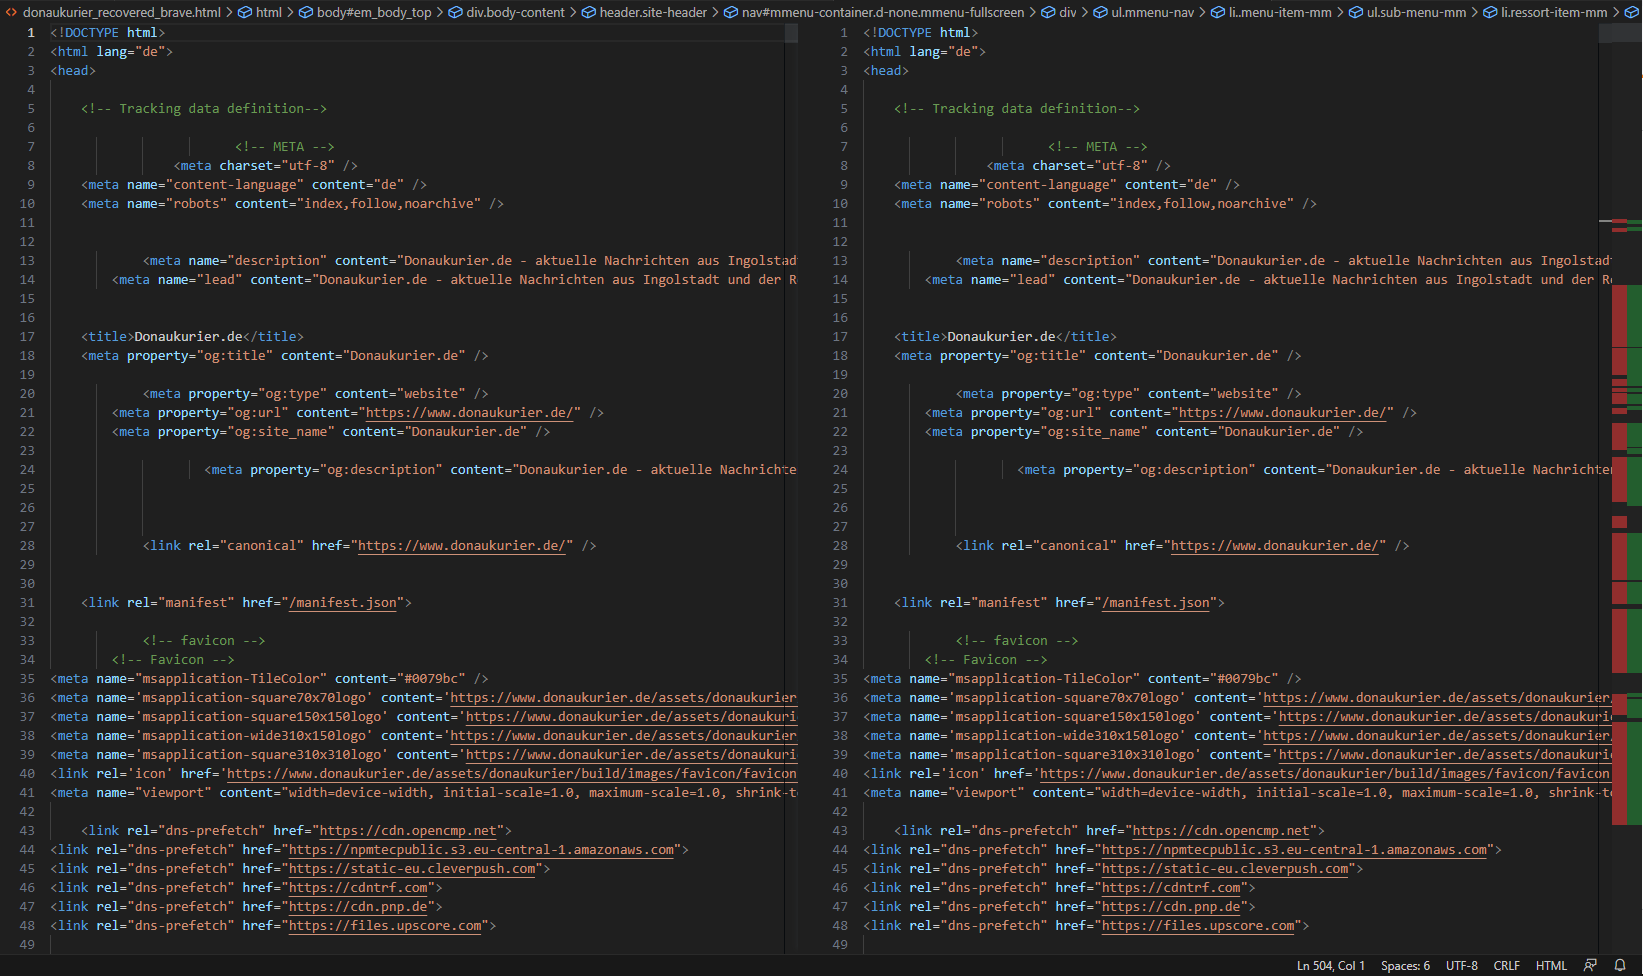
\includegraphics[width=\textwidth]{Donaukurier1.png}
	\caption{Brave: Ausschnitt aus VS Code mit dem Vergleich der beiden Donaukurier Webseiten}
	\label{pic:compareHTMLs}
\end{figure}

\paragraph*{Yara-Regel \glqq{}Suchbegriffe\grqq{}}\label{chap:ergebnisse-brave-uncommon-locations-volatility-suchbegriffe}  
Abbildung \ref{chart:brave-volatility-keywords} zeigt, dass alle der vier Suchbegriffe jeweils gefunden wurden, jedoch nur im zweiten RAM-Dump, also nach der Durchführung des Browsing-Szenarios bei noch geöffnetem Browser. Der String \glqq{}pfaffenhofen\grqq{} wurde dabei am häufigsten mit 1447 Treffern, \glqq{}nanoradar\grqq{} am seltensten mit nur 51 Suchergebnissen gefunden. Dabei wurden auch alle Suchbegriffe rein in Brave-Prozessen ausfindig gemacht.

\begin{table}[h!]
	\resizebox{\linewidth}{!}{
		\begin{tabular}{l}	
			\begin{tikzpicture}
				\begin{axis}[
					xbar,
					width=12cm, 
					height=3cm, 
					ylabel style={align=center}, ylabel=\textbf{pfaffenhofen},
					y=0.75cm,
					symbolic y coords={RAM-Dump 3, RAM-Dump 2, RAM-Dump 1},
					label style={font=\small},
					tick label style={font=\small},
					ytick=data,
					xticklabels={,,},
					xmin = 0,
					xmax = 1700,
					nodes near coords, 
					nodes near coords align={horizontal},
					nodes near coords style={font=\tiny},
					nodes near coords={\pgfmathfloatifflags{\pgfplotspointmeta}{0}{}{\pgfmathprintnumber{\pgfplotspointmeta}}},
					bar width=.17cm,
					enlarge y limits={abs=2*\pgfplotbarwidth},
					scaled x ticks=false,
					legend style={
						at={(0.5,-0.1)},
						anchor=north
					},
					legend columns=3,
					yminorgrids = true,minor tick num=1
					]
					\addplot coordinates {
						(0,RAM-Dump 3) (1447,RAM-Dump 2) (0,RAM-Dump 1)
					};
					\addplot coordinates {
						(0,RAM-Dump 3) (0,RAM-Dump 2) (0,RAM-Dump 1)
					};
				\end{axis}
			\end{tikzpicture}
			\\[-7pt]
			\begin{tikzpicture}
				\begin{axis}[
					xbar,
					width=12cm, 
					height=3cm, 
					ylabel style={align=center}, ylabel=\textbf{nanoradar},
					y=0.75cm,
					symbolic y coords={RAM-Dump 3, RAM-Dump 2, RAM-Dump 1},
					label style={font=\small},
					tick label style={font=\small},
					ytick=data,
					xticklabels={,,},
					xmin = 0,
					xmax = 1700,
					nodes near coords, 
					nodes near coords align={horizontal},
					nodes near coords style={font=\tiny},
					nodes near coords={\pgfmathfloatifflags{\pgfplotspointmeta}{0}{}{\pgfmathprintnumber{\pgfplotspointmeta}}},
					bar width=.17cm,
					enlarge y limits={abs=2*\pgfplotbarwidth},
					scaled x ticks=false,
					legend style={
						at={(0.5,-0.1)},
						anchor=north
					},
					legend columns=3,
					yminorgrids = true,minor tick num=1
					]
					\addplot coordinates {
						(0,RAM-Dump 3)  (518,RAM-Dump 2) (0,RAM-Dump 1)
					};
					\addplot coordinates {
						(0,RAM-Dump 3)  (0,RAM-Dump 2) (0,RAM-Dump 1)
					};
				\end{axis}
			\end{tikzpicture}
			\\[-7pt]
			\begin{tikzpicture}
				\begin{axis}[
					xbar,
					width=12cm, 
					height=3cm, 
					ylabel style={align=center}, ylabel=\textbf{mooserliesl},
					y=0.75cm,
					symbolic y coords={RAM-Dump 3, RAM-Dump 2, RAM-Dump 1},
					label style={font=\small},
					tick label style={font=\small},
					ytick=data,
					xticklabels={,,},
					xmin = 0,
					xmax = 1700,
					nodes near coords, 
					nodes near coords align={horizontal},
					nodes near coords style={font=\tiny},
					nodes near coords={\pgfmathfloatifflags{\pgfplotspointmeta}{0}{}{\pgfmathprintnumber{\pgfplotspointmeta}}},
					bar width=.17cm,
					enlarge y limits={abs=2*\pgfplotbarwidth},
					scaled x ticks=false,
					legend style={
						at={(0.5,-0.1)},
						anchor=north
					},
					legend columns=3,
					yminorgrids = true,minor tick num=1
					]
					\addplot coordinates {
						(0,RAM-Dump 3)  (51,RAM-Dump 2) (0,RAM-Dump 1)
					};
					\addplot coordinates {
						(0,RAM-Dump 3)  (0,RAM-Dump 2) (0,RAM-Dump 1)
					};
				\end{axis}
			\end{tikzpicture}
			\\[-7pt]
			\begin{tikzpicture}
				\begin{axis}[
					xbar,
					width=12cm, 
					height=3cm, 
					ylabel style={align=center}, ylabel=\textbf{mallofamerica},
					y=0.75cm,
					symbolic y coords={RAM-Dump 3, RAM-Dump 2, RAM-Dump 1},
					label style={font=\small},
					tick label style={font=\small},
					ytick=data,
					xticklabels={,,},
					xmin = 0,
					xmax = 1700,
					nodes near coords, 
					nodes near coords align={horizontal},
					nodes near coords style={font=\tiny},
					nodes near coords={\pgfmathfloatifflags{\pgfplotspointmeta}{0}{}{\pgfmathprintnumber{\pgfplotspointmeta}}},
					bar width=.17cm,
					enlarge y limits={abs=2*\pgfplotbarwidth},
					scaled x ticks=false,
					legend style={
						at={(0.5,-0.1)},
						anchor=north
					},
					legend columns=3,
					yminorgrids = true,minor tick num=1
					]
					\addplot coordinates {
						(0,RAM-Dump 3)  (108,RAM-Dump 2) (0,RAM-Dump 1)
					};
					\addplot coordinates {
						(0,RAM-Dump 3)  (0,RAM-Dump 2) (0,RAM-Dump 1)
					};
					\legend{brave.exe, Andere Prozesse}
				\end{axis}
			\end{tikzpicture}
		\end{tabular}
	}
	\captionof{figure}{Brave: Anzahl gefundener Suchbegriffe im RAM}
	\label{chart:brave-volatility-keywords}
\end{table}
%TODO Vergleich Google Duckduckgo

\paragraph*{Yara-Regel \glqq{}URLs\grqq{}}\label{chap:ergebnisse-brave-uncommon-locations-volatility-urls}

Wie in Abbildung \ref{chart:brave-volatility-urls} gezeigt, konnten alle URLs im RAM nachgewiesen werden. Bei \glqq{}donaukurier.de\grqq{} gab es sogar einen Treffer im dritten RAM-Dump, alle anderen waren nur im zweiten Speicherabbild auffindbar. Darunter waren mit insgesamt 3514 Artefakten am meisten Donaukurier-URLs, wobei sechs davon in anderen Prozessen neben Brave gefunden wurden. Sehr präsent war hier der Prozess \glqq{}NisSrv.exe\grqq{}. Dieser ist ein Teil des Microsoft Defenders \cite{pogonin2022microsoft}. Dies lässt sich evtl. dadurch erklären, dass dieser im Hintergrund den Datenverkehr mitliest und prüft, ob bösartige Software unsicheren Netzwerkverkehr tätigt.

\begin{table}[h!]
	\resizebox{\linewidth}{!}{
		\begin{tabular}{r}	
			\begin{tikzpicture}
				\begin{axis}[
					xbar,
					width=12cm, 
					height=3cm, 
					ylabel style={align=center}, ylabel=\textbf{unitree.com},
					y=0.75cm,
					symbolic y coords={RAM-Dump 3, RAM-Dump 2, RAM-Dump 1},
					label style={font=\small},
					tick label style={font=\small},
					ytick=data,
					xticklabels={,,},
					xmin = 0,
					xmax = 3800,
					nodes near coords, 
					nodes near coords align={horizontal},
					nodes near coords style={font=\tiny},
					nodes near coords={\pgfmathfloatifflags{\pgfplotspointmeta}{0}{}{\pgfmathprintnumber{\pgfplotspointmeta}}},
					bar width=.17cm,
					enlarge y limits={abs=2*\pgfplotbarwidth},
					scaled x ticks=false,
					legend style={
						at={(0.5,-0.1)},
						anchor=north
					},
					legend columns=3,
					yminorgrids = true,minor tick num=1
					]
					\addplot coordinates {
						(0,RAM-Dump 3) (2788,RAM-Dump 2) (0,RAM-Dump 1)
					};
					\addplot coordinates {
						(0,RAM-Dump 3) (1,RAM-Dump 2) (0,RAM-Dump 1)
					};
				\end{axis}
			\end{tikzpicture}
			\\[-7pt]
			\begin{tikzpicture}
				\begin{axis}[
					xbar,
					width=12cm, 
					height=3cm, 
					ylabel style={align=center}, ylabel=\textbf{mooserliesl}\\\textbf{.de},
					y=0.75cm,
					symbolic y coords={RAM-Dump 3, RAM-Dump 2, RAM-Dump 1},
					label style={font=\small},
					tick label style={font=\small},
					ytick=data,
					xticklabels={,,},
					xmin = 0,
					xmax = 3800,
					nodes near coords, 
					nodes near coords align={horizontal},
					nodes near coords style={font=\tiny},
					nodes near coords={\pgfmathfloatifflags{\pgfplotspointmeta}{0}{}{\pgfmathprintnumber{\pgfplotspointmeta}}},
					bar width=.17cm,
					enlarge y limits={abs=2*\pgfplotbarwidth},
					scaled x ticks=false,
					legend style={
						at={(0.5,-0.1)},
						anchor=north
					},
					legend columns=3,
					yminorgrids = true,minor tick num=1
					]
					\addplot coordinates {
						(0,RAM-Dump 3) (884,RAM-Dump 2) (0,RAM-Dump 1)
					};
					\addplot coordinates {
						(0,RAM-Dump 3) (1,RAM-Dump 2) (0,RAM-Dump 1)
					};
				\end{axis}
			\end{tikzpicture}	
			\\[-7pt]
			\begin{tikzpicture}
				\begin{axis}[
					xbar,
					width=12cm, 
					height=3cm, 
					ylabel style={align=center}, ylabel=\textbf{mallofamerica}\\\textbf{.com},
					y=0.75cm,
					symbolic y coords={RAM-Dump 3, RAM-Dump 2, RAM-Dump 1},
					label style={font=\small},
					tick label style={font=\small},
					ytick=data,
					xticklabels={,,},
					xmin = 0,
					xmax = 3800,
					nodes near coords, 
					nodes near coords align={horizontal},
					nodes near coords style={font=\tiny},
					nodes near coords={\pgfmathfloatifflags{\pgfplotspointmeta}{0}{}{\pgfmathprintnumber{\pgfplotspointmeta}}},
					bar width=.17cm,
					enlarge y limits={abs=2*\pgfplotbarwidth},
					scaled x ticks=false,
					legend style={
						at={(0.5,-0.1)},
						anchor=north
					},
					legend columns=3,
					yminorgrids = true,minor tick num=1
					]
					\addplot coordinates {
						(0,RAM-Dump 3) (2943,RAM-Dump 2) (0,RAM-Dump 1)
					};
					\addplot coordinates {
						(0,RAM-Dump 3) (1,RAM-Dump 2) (0,RAM-Dump 1)
					};
				\end{axis}
			\end{tikzpicture}
			\\[-7pt]
			\begin{tikzpicture}
				\begin{axis}[
					xbar,
					width=12cm, 
					height=3cm, 
					ylabel style={align=center}, ylabel=\textbf{donaukurier}\\\textbf{.de},
					y=0.75cm,
					symbolic y coords={RAM-Dump 3, RAM-Dump 2, RAM-Dump 1},
					label style={font=\small},
					tick label style={font=\small},
					ytick=data,
					xticklabels={,,},
					xmin = 0,
					xmax = 3800,
					nodes near coords, 
					nodes near coords align={horizontal},
					nodes near coords style={font=\tiny},
					nodes near coords={\pgfmathfloatifflags{\pgfplotspointmeta}{0}{}{\pgfmathprintnumber{\pgfplotspointmeta}}},
					bar width=.17cm,
					enlarge y limits={abs=2*\pgfplotbarwidth},
					scaled x ticks=false,
					legend style={
						at={(0.5,-0.1)},
						anchor=north
					},
					legend columns=3,
					yminorgrids = true,minor tick num=1
					]
					\addplot coordinates {
						(0,RAM-Dump 3) (3508,RAM-Dump 2) (0,RAM-Dump 1)
					};
					\addplot coordinates {
						(5,RAM-Dump 3) (6,RAM-Dump 2) (0,RAM-Dump 1)
					};
					\legend{brave.exe, Andere Prozesse}
				\end{axis}
			\end{tikzpicture}		
		\end{tabular}
	}
	\captionof{figure}{Brave: Anzahl gefundener URLs im RAM}
	\label{chart:brave-volatility-urls}
\end{table}

\paragraph*{Yara-Regel \glqq{}E-Mail\grqq{}}\label{chap:ergebnisse-brave-uncommon-locations-volatility-email}

Wie in Abbildung \ref{chart:brave-volatility-mail} dargestellt, wurden im zweiten als auch im dritten Arbeitsspeicherabbild Artefakte bzgl. der Yara-Regel \glqq{}E-Mail\grqq{} gefunden. Davon waren die meisten bei der E-Mail-Adresse \glqq{}computerforensikvl@gmail.com\grqq{} mit insgesamt 134 Suchtreffern vorhanden. Neun dieser waren aus anderen Prozessen, die restlichen 125 waren direkt in einem Speicherbereich des Brave-Browsers zu finden. Bei dieser wurde auch noch ein Artefakt im dritten RAM-Dump gefunden im Speicherbereich des dwm.exe Prozesses, welcher zuvor bereits angesprochen wurde. Am wenigsten Suchtreffer hab es bei dem Betrefftext.

%TODO Vergleich mit Chrome bzgl. Anzahl der Hits entweder hier oder später

\paragraph{Yara-Regel \glqq{}DK-Logo\grqq{}}\label{chap:ergebnisse-brave-uncommon-locations-volatility-dklogo} 

Auch bei Brave wurde wieder in den Arbeitsspeicherabbildern nach den Bytes des Donaukurier-Logos gesucht. Hier kam es zu drei Treffern im zweiten RAM-Dump, was in der Abbildung \ref{chart:brave-volatility-image} zu erkennen ist.

\begin{table}[h!]
	\resizebox{\linewidth}{!}{
		\begin{tabular}{r}
			\begin{tikzpicture}
				\begin{axis}[
					xbar stacked,
					width=18cm, 
					height=12cm, 
					ylabel style={align=center}, ylabel=\textbf{Donaukurier Logo}\\\textbf{(Hexadezimal)},
					y=1cm,
					symbolic y coords={RAM-Dump 3, RAM-Dump 2, RAM-Dump 1},
					ytick=data,
					xticklabels={,,},
					xmin = 0,
					xmax = 4,
					nodes near coords, 
					nodes near coords align={horizontal},
					legend style={
						at={(0.5,-0.1)},
						anchor=north
					},
					legend columns=2
					]
					\addplot coordinates {
						(0,RAM-Dump 3) (3,RAM-Dump 2) (0,RAM-Dump 1)
					};
					\addplot coordinates {
						(0,RAM-Dump 3) (0,RAM-Dump 2) (0,RAM-Dump 1)
					};
					\legend{brave.exe, Andere Prozesse}
				\end{axis}
			\end{tikzpicture}
		\end{tabular}
	}
	\captionof{figure}{Brave: Anzahl gefundener Hexadezimalwerte des Donaukurier-Logos im RAM}
	\label{chart:brave-volatility-image}
\end{table}

\vspace*{-0.5cm}

\subsection*{Registry}\label{chap:ergebnisse-brave-uncommon-locations-registry} 

Bei der Registry konnten weder in den Process Monitor Logs noch durch die Analyse der verschiedenen Hives Artefakte gefunden werden. Weitergehende Informationen zu den Schreiboperationen und der Stringsuche in den verschiedenen Hives ist in Anhang \ref{chap:anhang-brave-registry} zu finden.

\begin{table}[h!]
	\resizebox{\linewidth}{!}{
		\begin{tabular}{r}	
			\begin{tikzpicture}
				\begin{axis}[
					xbar,
					width=12cm, 
					height=3cm, 
					ylabel style={align=center}, ylabel=\textbf{Betrefftext},
					y=0.75cm,
					symbolic y coords={RAM-Dump 3, RAM-Dump 2, RAM-Dump 1},
					label style={font=\small},
					tick label style={font=\small},
					ytick=data,
					xticklabels={,,},
					xmin = 0,
					xmax = 150,
					nodes near coords, 
					nodes near coords align={horizontal},
					nodes near coords style={font=\tiny},
					nodes near coords={\pgfmathfloatifflags{\pgfplotspointmeta}{0}{}{\pgfmathprintnumber{\pgfplotspointmeta}}},
					bar width=.17cm,
					enlarge y limits={abs=2*\pgfplotbarwidth},
					scaled x ticks=false,
					legend style={
						at={(0.5,-0.1)},
						anchor=north
					},
					legend columns=3,
					yminorgrids = true,minor tick num=1
					]
					\addplot coordinates {
						(0,RAM-Dump 3) (30,RAM-Dump 2) (0,RAM-Dump 1)
					};
					\addplot coordinates {
						(0,RAM-Dump 3) (0,RAM-Dump 2) (0,RAM-Dump 1)
					};
					%				\legend{firefox.exe, Andere Prozesse}
				\end{axis}
			\end{tikzpicture}
			\\[-7pt]
			\begin{tikzpicture}
				\begin{axis}[
					xbar,
					width=12cm, 
					height=3cm, 
					ylabel style={align=center}, ylabel=\textbf{Mailtext},
					y=0.75cm,
					symbolic y coords={RAM-Dump 3, RAM-Dump 2, RAM-Dump 1},
					label style={font=\small},
					tick label style={font=\small},
					ytick=data,
					xticklabels={,,},
					xmin = 0,
					xmax = 150,
					nodes near coords, 
					nodes near coords align={horizontal},
					nodes near coords style={font=\tiny},
					nodes near coords={\pgfmathfloatifflags{\pgfplotspointmeta}{0}{}{\pgfmathprintnumber{\pgfplotspointmeta}}},
					bar width=.17cm,
					enlarge y limits={abs=2*\pgfplotbarwidth},
					scaled x ticks=false,
					legend style={
						at={(0.5,-0.1)},
						anchor=north
					},
					legend columns=3,
					yminorgrids = true,minor tick num=1
					]
					\addplot coordinates {
						(0,RAM-Dump 3) (125,RAM-Dump 2) (0,RAM-Dump 1)
					};
					\addplot coordinates {
						(0,RAM-Dump 3) (0,RAM-Dump 2) (0,RAM-Dump 1)
					};
					%				\legend{firefox.exe, Andere Prozesse}
				\end{axis}
			\end{tikzpicture}	
			\\[-7pt]
			\begin{tikzpicture}
				\begin{axis}[
					xbar,
					width=12cm, 
					height=3cm, 
					ylabel style={align=center}, ylabel=\textbf{Vorlesung23!}\\\textbf{(Passwort)},
					y=0.75cm,
					symbolic y coords={RAM-Dump 3, RAM-Dump 2, RAM-Dump 1},
					label style={font=\small},
					tick label style={font=\small},
					ytick=data,
					xticklabels={,,},
					xmin = 0,
					xmax = 150,
					nodes near coords, 
					nodes near coords align={horizontal},
					nodes near coords style={font=\tiny},
					nodes near coords={\pgfmathfloatifflags{\pgfplotspointmeta}{0}{}{\pgfmathprintnumber{\pgfplotspointmeta}}},
					bar width=.17cm,
					enlarge y limits={abs=2*\pgfplotbarwidth},
					scaled x ticks=false,
					legend style={
						at={(0.5,-0.1)},
						anchor=north
					},
					legend columns=3,
					yminorgrids = true,minor tick num=1
					]
					\addplot coordinates {
						(0,RAM-Dump 3) (0,RAM-Dump 2) (0,RAM-Dump 1)
					};
					\addplot coordinates {
						(0,RAM-Dump 3) (0,RAM-Dump 2) (0,RAM-Dump 1)
					};
					%				\legend{firefox.exe, Andere Prozesse}
				\end{axis}
			\end{tikzpicture}
			\\[-7pt]
			\begin{tikzpicture}
				\begin{axis}[
					xbar,
					width=12cm, 
					height=3cm, 
					ylabel style={align=center}, ylabel=\textbf{computerforensikvl}\\\textbf{@gmail.com},
					y=0.75cm,
					symbolic y coords={RAM-Dump 3, RAM-Dump 2, RAM-Dump 1},
					label style={font=\small},
					tick label style={font=\small},
					ytick=data,
					xticklabels={,,},
					xmin = 0,
					xmax = 150,
					nodes near coords, 
					nodes near coords align={horizontal},
					nodes near coords style={font=\tiny},
					nodes near coords={\pgfmathfloatifflags{\pgfplotspointmeta}{0}{}{\pgfmathprintnumber{\pgfplotspointmeta}}},
					bar width=.17cm,
					enlarge y limits={abs=2*\pgfplotbarwidth},
					scaled x ticks=false,
					legend style={
						at={(0.5,-0.1)},
						anchor=north
					},
					legend columns=3,
					yminorgrids = true,minor tick num=1
					]
					\addplot coordinates {
						(0,RAM-Dump 3) (125,RAM-Dump 2) (0,RAM-Dump 1)
					};
					\addplot coordinates {
						(1,RAM-Dump 3) (9,RAM-Dump 2) (0,RAM-Dump 1)
					};
					%				\legend{firefox.exe, Andere Prozesse}
				\end{axis}
			\end{tikzpicture}	
			\\[-7pt]
			\begin{tikzpicture}
				\begin{axis}[
					xbar,
					width=12cm, 
					height=3cm, 
					ylabel style={align=center}, ylabel=\textbf{chs3702}\\\textbf{@thi.de},
					y=0.75cm,
					symbolic y coords={RAM-Dump 3, RAM-Dump 2, RAM-Dump 1},
					label style={font=\small},
					tick label style={font=\small},
					ytick=data,
					xticklabels={,,},
					xmin = 0,
					xmax = 150,
					nodes near coords, 
					nodes near coords align={horizontal},
					nodes near coords style={font=\tiny},
					nodes near coords={\pgfmathfloatifflags{\pgfplotspointmeta}{0}{}{\pgfmathprintnumber{\pgfplotspointmeta}}},
					bar width=.17cm,
					enlarge y limits={abs=2*\pgfplotbarwidth},
					scaled x ticks=false,
					legend style={
						at={(0.5,-0.1)},
						anchor=north
					},
					legend columns=3,
					yminorgrids = true,minor tick num=1
					]
					\addplot coordinates {
						(0,RAM-Dump 3) (61,RAM-Dump 2) (0,RAM-Dump 1)
					};
					\addplot coordinates {
						(0,RAM-Dump 3) (0,RAM-Dump 2) (0,RAM-Dump 1)
					};
					%				\legend{firefox.exe, Andere Prozesse}
				\end{axis}
			\end{tikzpicture}
			\\[-7pt]
			\begin{tikzpicture}
				\begin{axis}[
					xbar,
					width=12cm, 
					height=3cm, 
					ylabel style={align=center}, ylabel=\textbf{cas0597}\\\textbf{@thi.de},
					y=0.75cm,
					symbolic y coords={RAM-Dump 3, RAM-Dump 2, RAM-Dump 1},
					label style={font=\small},
					tick label style={font=\small},
					ytick=data,
					xticklabels={,,},
					xmin = 0,
					xmax = 150,
					nodes near coords, 
					nodes near coords align={horizontal},
					nodes near coords style={font=\tiny},
					nodes near coords={\pgfmathfloatifflags{\pgfplotspointmeta}{0}{}{\pgfmathprintnumber{\pgfplotspointmeta}}},
					bar width=.17cm,
					enlarge y limits={abs=2*\pgfplotbarwidth},
					scaled x ticks=false,
					legend style={
						at={(0.5,-0.1)},
						anchor=north
					},
					legend columns=3,
					yminorgrids = true,minor tick num=1
					]
					\addplot coordinates {
						(0,RAM-Dump 3) (67,RAM-Dump 2) (0,RAM-Dump 1)
					};
					\addplot coordinates {
						(0,RAM-Dump 3) (0,RAM-Dump 2) (0,RAM-Dump 1)
					};
					\legend{brave.exe, Andere Prozesse}
				\end{axis}
			\end{tikzpicture}
			%	\begin{axis}[]
				%	\legend{Logfile 1, Logfile 2}
				%	\end{axis}
			
		\end{tabular}
	}
	\captionof{figure}{Brave: Anzahl gefundener E-Mail Artefakte im RAM}
	\label{chart:brave-volatility-mail}
\end{table}
%TODO Carl ausbessern p(f)affenhofen + computerforensik(vl)

%EOF